\documentclass[../main.tex]{subfiles}
\documentclass{book}
\usepackage{listings}
\usepackage{amsmath,amsthm,amssymb}


\begin{document}

\subsubsection{EXAMPLE 13.3:} Let $\Omega$ denote the annular domain $\left\{ p = (x,y) \in  R^2 \leqslant \Vert p \Vert_2 \leqslant 2 \right\}$  Use MATLAB to create and plot a triangulation of $\Omega$ having between 200 
and 400 nodes that are more or less uniformly distributed.
\\
\\
SOLUTION: We use a node deployment strategy that is based on that of Method 
2 of part (a) of the last example, distributing nodes on concentric circles starting at $\Vert p \Vert_2 = 1$ and ending at $\Vert p \Vert_2 = 2$. Letting, as before, $\delta$ denote the (approximate) 
common gap size between nodes (and the circles of node deployment), the average 
radius will be (roughly) 3/2, so that the average circumference will be 
$2\pi\left( 3/2 \right) = 3\pi$. The average number of nodes on a circle of deployment will thus 
be $3\pi/\delta$ and the number of such circles will be (roughly) $1/\delta$. This gives the following approximation for the total number of nodes: $(3\pi/\delta)\cdot(1/\delta)-3\pi/\delta$. 
Setting this equal to 350 and solving for delta gives us a good value to use: 
$\delta = 0.164097...$.
\\
\begin{lstlisting}[numbers=none,frame=none]
>> delta=sqrt(3*pi/350); 
nodecount=l; ncirc=floor(1/delta); radgap=l/ncirc; 

for i=0:ncirc 
	rad=l+i*radgap; nnodes-floor(2*pi*rad/delta); anglegap=2*pi/nnodes; 
	for k=l.-nnodes 
	x(nodecount)=rad*cos(k*anglegap); y(nodecount)=rad*sin(k*anglegap) ; 
	  nodecount = nodecount+1; 
	end 
end 
>> tri=delaunay(x,y); trimesh(tri,x,y), axis ('equal') 
>> size(x) 
->ans = 1 399
\end{lstlisting}
We are just under the desired upper bound on the number of nodes (if we had gone 
over, we could just increase $\delta$ a bit and try again. The resulting plot of the 
triangulation is shown in Figure 13.16(a).
\\
\\ 
Locating and deleting the unwanted triangles in Figure 13.16(a) would be an 
arduous task. The problem could be greatly simplified if we were to throw in an 
extra "ghost node" at (0,0). This is done by simply entering 
\begin{lstlisting}[numbers=none,frame=none]
>> x(400)=0 ; y(400)=0 ; 
>> tri=delaunay(x,y); trimesh(tri,x,y) , axis('equal')
\end{lstlisting}
The resulting triangulation shown in Figure 13.16(b) is much easier to work with. 
The triangles that need to get deleted are simply those that have (0,0) (node $\#$400) 
as one of their vertices. So we simply delete from the triangulation matrix all rows 
that contain the entry 400. It is very simple to tell MATLAB how to do this, after 
checking there are 722 triangles (elements). We will make use of the following 
"set difference" command:

\begin{center}
\begin{tabular}{|c|l|}
\hline
\texttt{c =} &If a and b are vectors, the output of this "set difference"\\
 \texttt{setdiff(a,b )} &command will be another vector c whose elements consist of\\
 \texttt{$\rightarrow$} &the different values of a that do not occur in b. \\
\hline
\end{tabular}
\end{center}
Here is a simple example: 
\\
\texttt{>> setdiff([ 3 1 2 3] , [2])->ans = 1 3}
\\
Now back to our problem; the following series of commands will produce the final 
triangulation of Figure 13.16(c). 
\\
\begin{lstlisting}
>> badelcount=l; 
for ell=l:722 
	if ismember(400,tri(ell,:)) 
	  badel(badelcount)=ell; 
	  badelcount=badelcount+1; 
	end 
end 
>> tri=tri(setdiff(1:722,badel),:); 
>> x=x(1:399); y=y(1:399); 
>> trimesh(tri,x,y), axis('equal') 

\end{lstlisting}
\begin{figure}[H]
    \centering
    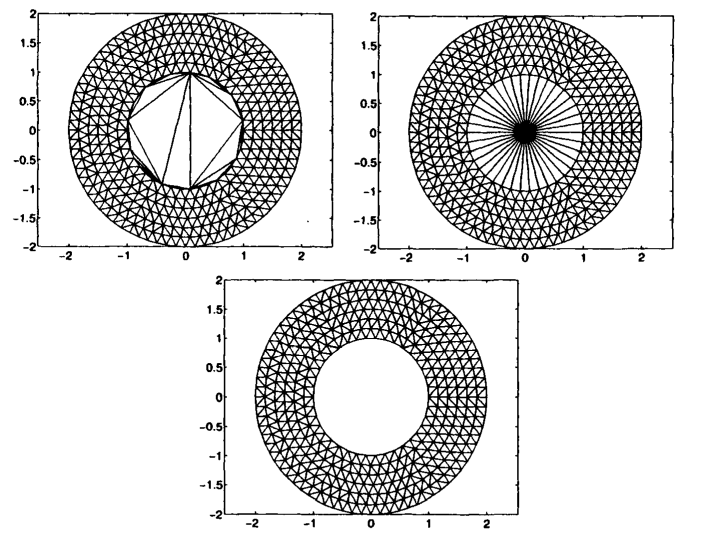
\includegraphics[width=0.7\linewidth]{1}
    \caption{\textsf{: (a) (upper left) The Delaunay triangulation obtained from a set of nodes in 
the annular domain$\left\{ p = (x,y) \in  R^2 \leqslant \Vert p \Vert_2 \leqslant 2 \right\}$ of Example 13.3. (b) (upper right) 
The Delaunay triangulation for the same set with one additional "ghost node" added at 
(0,0). (c) Resulting triangulation for the annulus. }}
    \label{pfig:ch13_1}
\end{figure}
The schemes introduced in the previous examples can be combined in various 
fashions to give a decent collection of strategies for triangulation of planar 
domains that will be sufficient for our purposes. The topic of mesh generation 
has been receiving a great deal of attention beginning in the 1990s. We will see 
later in this chapter that boundary value problems on domains with obtuse ($> \pi$) 
interior angles (see Figure 13.17 for two examples of such domains) usually 
require special attention with the numerical methods at corresponding boundary 
points. The next exercise for the reader asks the reader to construct suitable 
triangulations for such domains.
\\
EXERCISE FOR THE READER 13.4: Using a scheme similar to that of the 
solution of part (c) of Example 13.2, get MATLAB to create and plot 
triangulations each having between 500 and 1000 nodes for the two domains 
illustrated in Figure 13.17(a), (b), respectively. In each, arrange it so that the 
distribution of nodes increases near the special boundary point \textit{p} indicated in the illustration. For the domain of part (a), take the exterior angle to be 60$^\circ$; for the 
one of part (b), make up your own coordinates and dimensions.
\begin{figure}[H]
    \centering
    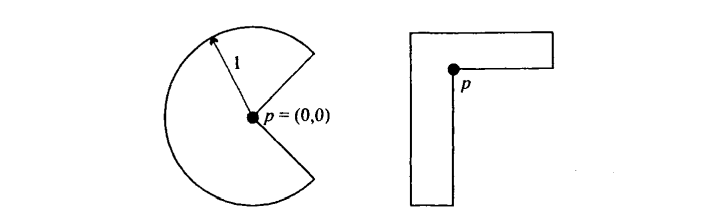
\includegraphics[width=0.7\linewidth]{2}
    \caption{\textsf{: (a), (b) A pair of domains possessing a boundary point $p$ with an obtuse 
interior angle. Such boundary points usually require extra care when boundary value 
problems on them are solved numerically. }}
    \label{pfig:ch13_1} 
\end{figure} 
In each of the triangulations done above, we tried to create them to meet most of 
the desired properties that were mentioned at the beginning of the chapter. There 
is one notable exception, however, that we did not even contemplate in our 
constructions. Namely, we made no efforts to arrange that the node numbers for 
any given triangle in the triangulations were reasonably close. (The constructions 
were already quite complicated without this and ?he Delaunay triangulation 
program left parts of the construction out of our control). The reason why this is a 
desirable property to have is that the resulting stiffness matrix will be banded (and 
hence sparse and easier to deal with). To get a rough idea of the relative 
numbering of the nodes, recall that MATLAB's function spy , introduced in 
Chapter 11, can gives us a "graph" of the nonzero entries of a matrix. For 
convenience, we give here a quick example reviewing its syntax. 

\begin{lstlisting}[numbers=none,frame=none]
>> d=ones(l,6) ; b=2*d(l:5);
>> A=diag(d)+diag(b, -1) 
\end{lstlisting}

A=  $\begin{array}{cccccc}
	1&0&0&0&0&0\\
	2&1&0&0&0&0\\
	0&2&1&0&0&0\\
	0&0&2&1&0&0\\	
	0&0&0&2&1&0\\
	0&0&0&0&2&1
\end{array}$
\\
\\
\\
\texttt{>> spy(A,'rx') $\%$ mark nonzero entrie s with red}\\
	\texttt{>>$\%$~~~~~~~~~~~~~~ x's; or use spy(A)}
\begin{figure}[h]
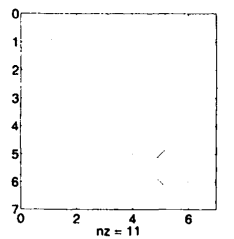
\includegraphics[width=0.4\linewidth]{3}
	\centering
	\label{pfig:ch13_1}
	\caption{\textsf{	
	A simple spy plot of a banded 6x6 matrix. 
The locations of nonzero entries are indicated by x's. The 
total number of nonzero entries (nz = 11) is indicated below 
the graph. The spy command is a useful tool for obtaining a 
quick understanding of the structure of a matrix, and, in 
particular, allows for quick detection of sparse and banded 
matrices.}}
\end{figure}
\\
The triangulation that we created in the solution of Example 13.2(c) had 1457 
nodes. The corresponding stiffness matrix A would thus be 1457$\times$1457. As in 
the one-dimensional FEM, we will see in the next section that the $a_ij$ entry (corresponding to node numbers $\#i$ and $\#j$) of the stiffness matrix will be given by 
a certain integral involving products of (gradients of) the corresponding basis 
functions $\Phi_i$, and $\Phi_j$. Throughout the text of this chapter, we will be restricting 
our attention to piecewise linear basis functions, and for such a basis function, say 
($\Phi_i$, it will be zero except on those elements that have node $\#i$ as one of their 
vertices. It follows that $a_ij$ will be zero unless nodes $\#i$ and $\#j$ are both vertices of 
the same triangle. In the following example, we will use this fact to find out all 
possible nonzero entries of the stiffness matrix, draw a spy diagram, and list the 
total number of possible nonzero entries. The way we will form this matrix is to 
simply put a positive integer at all entries that are possibly nonzero.
\\
\\
\textbf{EXAMPLE 13.4}: Let A denote the 1457$\times$1457 stiffness matrix for the 
triangulation obtained in Example 13.2(c) and with piecewise linear basis 
functions. Using the information above, construct a matrix M that will have 
positive integer entries where the corresponding entries of the stiffness matrix are 
zero, and zero entries where the stiffness matrix has zero entries.
\\
\\
SOLUTION: The way we will construct M will be similar to the so-called 
"assembly" method that we will use in the next section to build stiffness matrices. 
The construction will proceed element by element. More precisely, we begin with 
M being a 1457$\times$1457 matrix of zeros. We then run down the list of 
triangles/elements (all 2733 of them), and for each one we change the 
corresponding entry of the of the matrix ?/to equal 1 (these are the only entries of 
that stiffness matrix A that could be nonzero). If an element is represented by the 
three vertices: $\left[ i ~j ~ k \right]$, the entries we will bump up by one for this element would be the following nine entries $a_\alpha\beta$ where $\alpha$ and $\beta$ run through i,j, and k. This is a much more efficient scheme rather than constructing the nonzero elements directly (in which case for each one a search would need to be done over all elements to see if the corresponding pair of nodes share a common element).

Assuming the matrix \texttt{tri} obtained in the last example (for the Delaunay 
triangulation of the nodes in part (c)), the following commands will "assemble" a 
suitable matrix M, and then create a spy diagram of it (and hence also of the 
stiffness matrix). The spy diagram is shown in Figure 13.19. 
\begin{lstlisting}[numbers=none,frame=none]
>> M=zeros(1457); for c=l:2733 
	E=tri(c,:); 
	for i=l:3 
	for j=l:3 
		M(E(i),E(j))=M(E(i),E(j))+l; 
	end 
	end 
end 
>> spy(M,'b+') %or use spy(M) to use default  markers '.'
>> 9835/1457 2 ->ans = 0.0046 
\end{lstlisting}

\begin{figure}[H]
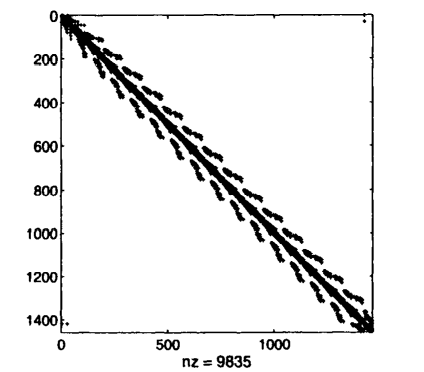
\includegraphics[width=0.9\linewidth]{4}
	\centering
	\label{pfig:ch13_1}
	\caption{A spy diagram of the stiffness matrix for Example 13.4. The possible 
nonzero entries account for only 0.46$\%$ of all of the entries, so this stiffness matrix is sparse 
as stiffness matrices usually are. The fuzzy patterns (top and bottom) correspond to the 
boundary nodes being added after the interior nodes. The number of such patterns is the 
number of master iterations in the node construction.}
\end{figure}
The last ratio is simply that of the nonzero entries to the total entries of M. Thus at 
most 0.46$\%$ of the entries in the stiffness matrix can be nonzero, and the matrix is 
indeed sparse. 
\\
\\
Can the reader explain the isolated four markers in the upper-right and lower-left 
of Figure 13.19? 
\\
\line(2,0){\textwidth}
\\
\textbf{EXERCISES 13.2}
\begin{enumerate}
    \item (a) For the hexagonal domain of Figure 13.5 with node coordinates as given by the matrix N 
following Figure 13.6, deploy between 1000 and 2000 nodes more or less uniformly throughout 
the domain and boundary and plot the nodal configuration. You should of course include the 
boundary nodes of Figure 13.5 but not necessarily the interior nodes ($\#$4, $\#$5). 
(b) Create a corresponding Delaunay triangularon and plot.
    \item Repeat parts (a) and (b) of Exercise 1, but this time let the nodes increase in density as one 
moves toward the boundary. 
    \item Repeat parts (a) and (b) of Exercise 1, but this time let the nodes increase in density as one 
approaches the exterior node $\#6$.
	\item Letting $\Omega$ denote the unit disk $\left\{ p = (x,y) \in  R^2 \leqslant \Vert p \Vert_2 \leqslant 2 \right\}$ of Example 13.2, use MATLAB to 
create and plot a triangulation of $\omega$ having between 1000 and 2000 nodes for which the nodes 
increase in density near the segment -$\pi/4  \leqslant \theta \leqslant \pi/4$ on the boundary, that is, near the (smaller) 
circular arc connecting the points $(\sqrt{2}/2,\pm \sqrt{2}/2)$ on the boundary. Let the node distribution elsewhere in the disk be more or less uniform. 
\\
\textbf{Suggestion:} Use the solution to part (c) of Example 13.2 for some relevant ideas. First deploy 
some nodes in a circle centered at (0,0), say $\Vert p \Vert_2 \leqslant 0.5$, then use a loop to deploy nodes in the 
annuli $An - \lbrace p: 1-2^n \leqslant \Vert p \Vert_2 \leqslant 1-2^{n+1} \rbrace, n = 1, 2,....$ As an indicator of closeness to circular 
arc (for points (xy)) in $A_n$ use the inequality $tan(y/x)\leqslant 1 + 2 \cdot 2^n"$.
	\item Repeat Exercise 4 with the modification that node distribution should increase near the 
boundary. For the portion of the boundary complementary to $-\pi/4 \leqslant \theta \leqslant \pi /4$ , make the rate 
of increase in node density to be roughly 10$\%$ compared to the rate of increase near the special 
portion.
	\item (a) Write an M-file, call it \texttt{[x y tri ] =circtr i (anglel, angle2, maxnodes)} that 
will do the following. The input variables \texttt{angle} l and \texttt{angle2} denote two angles on the unit 
circle such that $0 \leqslant angle2 - anglel < 2/pi$. The M-file will create a set of nodes, stored in the 
output variables x and y for the triangularon of the unit disk $p = \left\{(x,y) \in  R^2 : \Vert p \Vert_2 \leqslant 2 \right\}$ in a 
way analogous to the one explained in Exercise 4 (for the special case \texttt{angle = $-\pi/4$} and 
\texttt{angle2 = $\pi/4$} but with the total number of nodes deployed being between the input variable 
\texttt{maxnodes} and half of this variable. Thus \texttt{maxnodes} should be a positive integer, at least 
equal to, say, 20. The final output variable \texttt{tri} will be a three-column matrix corresponding to 
the Delaunay triangularon of the node set. Note that the syntax includes the possibility that 
anglel = angle2, in which case a triangularon similar to that done in Example 13.2(c) is 
required.
\\
(b) Use your program to redo Exercise 4.
\\
(c) Run your program, and plot the nodes and resulting triangulations for each of the following 
sets of input variables: 
\\
(i) anglel = $\pi/2$, angle2 = $5\pi/6$, maxnodes = 500 
\\
(ii) anglel = $-\pi$, angle2 = $\pi/2$, maxnodes = 1500 
\\
(iii) angle $7\pi/6$, angle2 = $11\pi/6$, maxnodes = 1200 
	\item (a) Write an M-file, call it \texttt{[x y tri ] =circtr i (anglel, angle2, maxnodes, r)} , that has the same syntax as that explained in Exercise 6, except that there is an additional 
input variable r which is to be a positive number less than 1 and the triangularon will be 
performed as explained in Exercise 5 (for the special case anglel = $-\pi/4$ and angle2 = $\pi/4$, 
and $r = 0.1$). The parameter r will denote the relative density that nodes are increasing as we 
near the complementary arc compared to when we near the arc anglel $<$ $\theta$ $<$ angle2.
\\ 
(b) Use your program to redo Exercise 5. 
\\
(c) Run your program, and plot the nodes and resulting triangulations for each of the following 
sets of input variables: 
\\
(i) anglel = $\pi/2$, angle2 = $5\pi/6$, maxnodes = 500, r=0.25
\\
(ii) anglel = $-\pi$, angle2 = $\pi/2$, maxnodes = 1500, r=0.25
\\
(iii) angle $7\pi/6$, angle2 = $11\pi/6$, maxnodes = 1200, r=0.025
	\item (\textit{Triangulating General Convex Polygons}) (a) Write an M-file, call it \texttt{[x y tri ] =unipolytr i (xv, yv, maxnodes)}, that will do the following. The input 
variables \texttt{xv} and \texttt{yv} denote the vectors corresponding to the x- and y-coordinates of vertices of a 
convex polygon which are assumed to be ordered in counterclockwise fashion around the 
boundary. The first vertex should also be the last vertex (to close the polygon). The last 
variable \texttt{maxnodes} denotes a positive integer, say, at least 20. The program will create a set of 
nodes for a triangulation of the polygon and its boundary that will be stored in the output 
variables x and y. The nodes are to be configured in a square pattern (cf, Method 1 of the 
solution to Example 13.2(a)) throughout the polygon and its boundary. The number of nodes 
deployed should be somewhere between \texttt{maxnodes} and half of this number. The third output variable \texttt{tri} denotes a 3-column matrix corresponding to the Delaunay triangularon for the 
node set which is constructed.
\\ 
(b) Use your program to redo Exercise 1. 
\\
(c) Run your program, and plot the nodes and resulting triangulations to obtain triangulations for 
each of the following convex polygons using between 200 and 400 nodes for each. 
\\
(i) The rectangle with vertices ($\pm1,\pm10$).
\\ 
(ii) The triangle with vertices (0,0), (1,0), (0,8). \\
(iii) A regular octagon unit sidelength. 
\\
(iv) The septagon with vertices (0,0), (2,0), (16,1), (16,4), (13,5),( 11,4), (1,3). 
\\
\textbf{Suggestion:} One way to view a convex polygon is that its set of points can be described as the 
intersection of all points in the plane which simultaneously lie on the correct side of each of its 
edges. Each such edge requirement can be written mathematically in the form $ax + by \leqslant c$ . Set 
up a grid of about maxnodes nodes in the rectangle $R = \lbrace\left( x,y\right) : min(xv) \leqslant x \leqslant min(xv), 
mm(yv) \geqslant y \geqslant mm(yv)\rbrace$,then use each of the edge requirements (put in form $ax + by < c$ to 
save boundary points for later) to decide with a loop which of these points should be interior 
points. Finally put nodes on the boundary with appropriate density. Make sure that there are no 
interior nodes that are too close to the boundary. That the number of nodes put in the polygon 
will satisfy the required bounds follows from the fact that the area of the polygon is at least half 
the area of the rectangle R (why?).
	\item[NOTE:]$(\textit{Triangulating General Polygons})$ Since any polygon can be decomposed into convex pieces, 
the program \texttt{unipolytri} of Exercise 8 can be used to essentially uniformly triangulate general 
polygons. For example, the polygon of Figure 13.17(b) is not convex but can be written as a union of 
two (convex) rectangles $R_1$, and $R_2$, that have corresponding areas $A_1$, and $A_2$. (There are a couple 
of ways to do this.) Suppose we wish to triangulate the region using somewhere between 500 and 1000 
nodes. We could run the program \texttt{unipolytri}  on $R_1$, using maxnodes to be about 
$1000A_1/(A_1 + A_2)$ and then on $R_2$ using maxnodes to be about $1000A_2/(A_1 + A_2)$. The ratios attempt 
at allocating an appropriate number of nodes to each piece. We can pretty much juxtapose these two 
node sets to arrive at a node set for the original polygon (after reindexing and deleting some nodes at 
the common interior interface boundary). This idea, and its extensions to greater numbers of convex 
pieces, is explored in the following three exercises. In particular, these exercises require the reader to 
have completed Exercise 8(a).
	\item Use the idea of the above note to redo Exercise for the Reader 13.4(b).
	\item Use the idea of the above note to triangulate, using between 400 and 800 nodes, the decagon 
that has the following vertices: $(\pm2,0)$, $(\pm1, 1)$, $(\pm2, \pm2)$. Plot both the node diagram as well as 
the triangularon. 
	\item Consider the symmetric (nonconvex) polygon consisting of the rectangle with vertices: 
$(\pm1,-1), (\pm1,0)$ with two (left and right) triangles with vertices: $(\pm1,1), (\pm1,0), (0,0)$ joined 
on top. 
\\
(a) Apply the method in the above note to triangulate this region by splitting it into the left and 
right halves (which are each convex). Display the node configuration and corresponding 
triangulation.
\\ 
(b) Apply the method in the above note to triangulate this region by splitting it into the 
following three convex pieces: the bottom rectangle, and the two triangles. Display the node 
configuration and corresponding triangulation. Does the density appear uniform? If not, 
explain, and adjust the ratios of node densities to correct the problem.
\\
	\item[] The next three exercises will involve triangulations of the domains having domains with curved 
boundaries illustrated in Figure 13.20.
\begin{figure}[H]
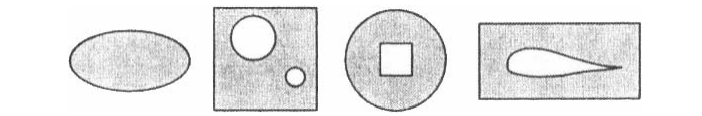
\includegraphics[width=0.9\linewidth]{5}
	\centering
	\label{pfig:ch13_5}
	\caption{Four domains with curved boundary portions: (from left) (a) An ellipse, (b) a 
square with two circular holes, (c) a disk with a square hole, (d) an airfoil removed from a rectangle}
\end{figure}
	\item Let the elliptical region $\omega$ of Figure 13.20(a) have equation (for its boundary): $x^2+4y^2-4$. 
Use MATLAB to create and plot triangulations of $\omega$ having between 400 and 800 nodes and 
with the following additional properties:
\\
(a) The nodes are more or less uniformly distributed with essentially a square grid (as in Method 
1 of part (a) in the solution of Example 13.2).
\\ 
(b) The nodes are deployed on concentric ellipses of the same eccentricity as the boundary 
ellipse (cf. Method 2 of part (a) in the solution of Example 13.2). 
\\
(c) The nodes are deployed in concentric ellipses (as in part (b)) but the density increases as we 
near the boundary (cf. part (b) in the solution of Example 13.2). 
\\
(d) The density of the nodes increases as we approach the interior point $(x,y) = (1,0)$ and such 
that between 20 and 30 nodes are deployed on the boundary (cf. Method 2 of part (a) in the 
solution of Example 13.2).
	\item Let the region $\omega$ of Figure 13.20(b) be specified as follows: The square (outside) boundary 
has equations: $x- 0,2, y- 0,2$ and the removed circles have the following centers and radii: 
upper left circle: center = (0.5, 1.5), radius - 0.25; lower right circle: center = (1.5, 0.5), radius 
= 0.1. Use MATLAB to create and plot triangulations of $\omega$ having between 400 and 800 
nodes and with the following additional properties:
\\
(a) The nodes are, more or less, uniformly distributed with essentially a square grid (cf. Method 
1 of part (a) in the solution of Example 13.2).
\\ 
(b) The density of the nodes increases as we near each of the two interior circle boundary 
portions and such that the square boundary has between 20 and 30 nodes.
	\item Let the region $\omega$ of Figure 13.20(c) be specified as follows: The outside circle has: center = 
(0, 0) and radius = 2; the inside square has equations: $x=\pm1,y=\pm1$ . Use MATLAB to create 
and plot triangulations of $\omega$ having between 400 and 800 nodes and with the following 
additional properties: 
\\
(a) The nodes are more or less uniformly distributed with essentially a square grid (cf. Method 1 
of part (a) in the solution of Example 13.2).
\\ 
(b) The nodes are deployed on concentric circles (to the outer boundary circle) and more or less 
uniformly distributed. 
\\
(c) The density of the nodes increases as we near any of the four corner points on the inside 
square boundary and the outside circle will have between 20 and 30 nodes. 
	\item Let $\omega$ denote the region of Figure 13.20(d). (a) Use MATLAB to plot an airfoil (the inside 
boundary of $\omega$ ) by setting up a set of points on the boundary of the foil. Then enter (as 
different vectors) the four vertices of an appropriate rectangle for the outer boundary of $\omega$. 
Your foil does not have to be identical with the one in the figure, but should more or less 
resemble it. We are more concerned here with triangulations rather than aerodynamics. Use 
MATLAB to create and plot triangulations of $\omega$ having between 400 and 800 nodes and with 
the following additional properties: 
\\
(b) The nodes are more or less uniformly distributed with essentially a square grid (cf. Method 
1 of part (a) in the solution of Example 13.2).
\\ 
(c) The density of the nodes increases as we near the airfoil (inside) part of the boundary and 
the outside rectangle will have between 20 and 30 nodes. See Figure 13.21 for examples of some related triangulations.
\\
\textbf{Suggestions:} To find appropriate x and y vectors for the foil, it is probably easiest to copy the 
figure down on graph paper and record a set of ordered (so it will plot correctly) vertices on the 
foil that is dense enough so as to render a decent plot. A more elaborate scheme would be to 
build up the boundary in terms of piecewise cubic splines whose derivatives match up on the 
interfaces (see the end of Section 10.5). MATLAB has a useful command for some of the tasks 
of this problem called \texttt{inpolygon} that will test if a given point lies within a given polygon: 
\begin{center}
\begin{tabular}{|c|l|}
\hline
 &If \texttt{xpoly} and \texttt{ypoly} are the x- and \\
 &y-coordinates of a set of vertices defining \\
 &a polygon and x and y are the coordinates \\
 \texttt{test = inpolygon(x, y, }&of any point in the plane, the output \texttt{test}\\
 \texttt{xpoly, ypoly)}&will be 1 if the point (xy) lies inside or on\\
 $\Rightarrow$&the boundary of the polygon and 0\\
 &otherwise. If x and y are vectors for a set\\
 &of points, the output \texttt{test} will be\\
 & a corresponding vector of 1's and/or O's.\\
 
\hline
\end{tabular}
\end{center}
\begin{figure}[H]
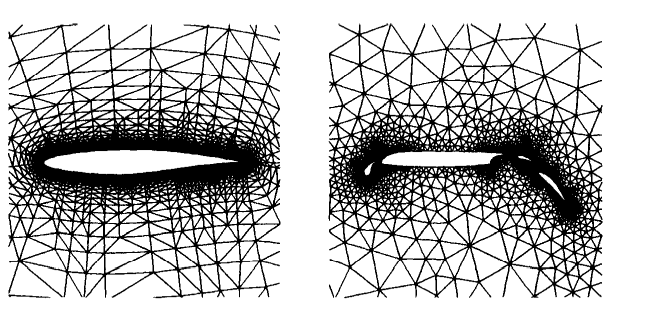
\includegraphics[width=0.9\linewidth]{6}
	\centering
	\label{pfig:ch13_6}
	\caption{Two triangulations of airfoils, (a) (left) A single component airfoil similar to that in 
Figure 13.20(d). The triangulation is structured using lines normal to the surface (with increasing 
density as we near the boundary), (b) A more complex airfoil with flaps. The triangulation is done in 
a way that the node density increases as we near crucial portions of the configuration$^8$}
\end{figure}
	\item[NOTE:](Rectangular Elements) For domains whose boundaries are made up of only vertical and 
horizontal segments, rectangular elements are often a popular choice for the FEM. A typical 
rectangular element is illustrated in Figure 13.22(a). If we use just the four vertices as the nodes of 
each rectangular element, then each local basis function has four degrees of freedom, so linear 
functions (whose graphs are planes) are no longer permissible to use as local basis functions. Popular 
choices for basis functions in this case are piecewise bilinear functions:
$$axy + bx + cy + d $$
These functions reduce to linear functions on any of the four edges of the rectangle so that continuity is 
assured across boundaries when elements are put together. Note that this would not be the case if the 
element were an arbitrary quadrilateral (if not all four sides are parallel to one of the axes). The next 
four exercises look more closely into rectangular elements. 
\footnotetext[8]{These two triangulations were created by Tim Barth (at the NASA Ames Research Center) and we 
thank him for his kind permission to include them in this text. Such triangulations of airfoils coupled 
with the FEM are used to model aerodynamics and design space and air vessels.}
\begin{figure}[H]
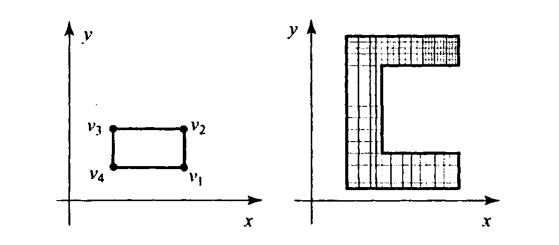
\includegraphics[width=0.9\linewidth]{7}
	\centering
	\label{pfig:ch13_7}
	\caption{(a) (left) Illustration of a typical rectangular element with its four nodes consisting 
of its vertices, (b) (right) Tessellation of a domain into rectangular elements.}
\end{figure}
	\item For the domain in Figure 13.22(b), let the outer vertices be (1,1), (7,1), (7,3), (3,3), (3,6), (7,6), 
(7,8), and (1,8). Tessellate the domain with square elements having unit sidelength (so there 
should be 30 elements).
\\
(a) Write down a formula for the basis function $\Theta_{(2,2)}$(x,y) corresponding to the interior node 
(2,2).
\\ 
(b) Use MATLAB to draw a three-dimensional graph of this basis function. 
\\
(c) Repeat parts (a) and (b) for the basis function $\Theta_{(1,1)}$(x,y) corresponding to the interior node 
(1,1).
\\ 
(d) Are these basis functions differentiable (smooth) across all edges of adjacent elements? (It 
was already pointed out that they are continuous across edges, and this should be evidenced 
from the graphs.)
	\item Let the domain in Figure 13.22(b) have the vertices and tessellation of the last exercise. On this 
domain, consider the following function:

$$f(x,y)=\left\{\begin{matrix}
[(x-1)/2]^2 & if~y\leq 3,\\ 
[(x-1)/2]^2 (2/3)|y-9/2|,&if~ 3\leq y \leq 9/2, \\ 
-[(x-1)/2]^2 (2/3)|y-9/2|, & if~9/2\leq y\leq 6, \\ 
-[(x-1)/2]^2, & if~y\geq 6,
\end{matrix}\right.$$
(a) Use MATLAB to draw a three-dimensional graph of this function.
\\ 
(b) Use MATLAB to draw a three-dimensional graph of the finite element interpolant to this 
function using the basis functions (Exercise 16) for the square elements of the tessellation. Note 
that this approximation is simply the function:
\\
$$f(1,1)\Theta_{(1,1)}(x,y)+f(1,2)\Theta_{(1,2)}(x,y)+\cdots$$
where each term of the sum corresponds to a node of the tessellation.
\\ 
(c) Create and plot a corresponding approximation to f(x,y) that arises from the triangularon of 
the domain using 60 triangles, each square element giving rise to two triangular elements via the 
diagonal from lower left to upper right.
\\ 
(d) Repeat part (b) except this time use squares of sidelength 1/4 in the tessellation. (So there 
will be 16 times as many elements.)
\\ 
\textbf{Suggestion}: In parts (b) and (d), use the meshgri d command for each element and use the 
hol d on command. 
	\item The standard rectangular element has vertices $(\pm1,\pm1)$. (a) Show that the corresponding four 
local basis functions (viz. (7)) are given by the following formulas (the ordering of the nodes is 
as in Figure 13.22a):
\\
$$\rho_3(x,y) = (1/4)(1-x)(l+y), ~\rho_2(x,y) = (1/4)(1+x)(l+y)$$
$$\rho_3(x,y) = (1/4)(1-x)(l-y), ~\rho_1(x,y) = (1/4)(1+x)(l-y)$$
(The local basis function $\rho_i$ corresponds to the vertex $v_i$, and they are written with the same orientation as the vertices appear in the element.) 
\\
(b) Use MATLAB to draw three-dimensional graphs of each of these four local basis functions. 
	\item (a) Find formulas, as in Exercise 18, for the four local basis functions for a general rectangular element with vertices: $(a, b),(a+h, b),(a+h, b+k),(a, b+k)$. Your formulas will depend, of course, on the parameters $a, b, h$, and $k$.
(b) Find an affine mapping $(x, y)=F(\tilde{x}, \bar{y})$ that carries the standard rectangular element of Exercise 18 (thought of as lying in the $\tilde{x} \tilde{y}$-plane) onto the general rectangular element of part (a) (thought of as lying in the $x y$-plane). In matrix form the mapping can be written as $\left[\begin{array}{l}x \\ y\end{array}\right]=A\left[\begin{array}{l}\tilde{x} \\ \tilde{y}\end{array}\right]+v$, where $A$ is a $2 \times 2$ matrix and $v$ is a $2 \times 1$ vector. How is the determinant of the matrix $A$ related to the areas of the two rectangular elements?
Suggestion: For part (a), try first by trial and error for some simple specific parameters; let them get more general and look for patterns. For example, you might start with $a=-1, h=2$, $b=-1, k=1$. These parameters are very close to those of the standard element with one difference ( $h$ is 2 instead of 1 ). Next try changing $h$ to 3 , keeping all else fixed. Then use $a=$ $-1, h=1, b=-1, k=2$; finally change $a$ and $b$ to other values, etc. Alternatively, part (a) can be done quite elegantly using part (b). See Exercise 23 for the relevant idea.
	\item We define a planar domain $\Omega$ to be horizontally blocklike if it has the following form:
$$
\Omega=\{(x, y): a \leq x \leq b, 0 \leq y \leq \lambda(x)\} \text {, }
$$
where $\lambda(x)$ is a positive-valued step function on $a \leq x \leq b$, i.e., there is a partition of $a \leq x \leq b: a=a_{0}<a_{1}<a_{2}<\cdots<a_{n+1}=b$ into $n+1$ subintervals $I_{i}=\left[a_{i-1}, a_{i}\right] \quad(1 \leq i \leq n+1)$ and corresponding positive numbers $c_{i}(1 \leq i \leq n+1)$, such that $\lambda(x)$ can be written as: $\lambda(x)=c_{i} \Leftrightarrow x \in I_{i}(1 \leq i \leq n+1)$. A typical horizontally blocklike domain is illustrated in Figure 13.23.
\begin{figure}[H]
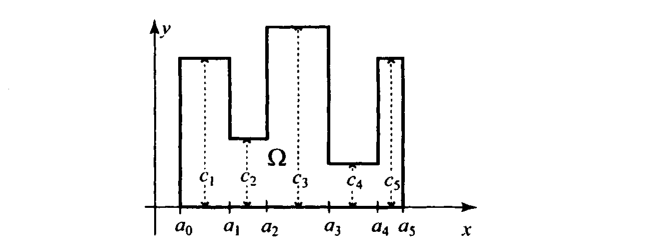
\includegraphics[width=0.9\linewidth]{8}
	\centering
	\label{pfig:ch13_8}
\end{figure}
\textbf{FIGURE 13.23:}  Illustration of a typical horizontally blocklike domain a for Exercise 20.
\\
(a) Write an M-file, \texttt{[x  y  nodes elems] =recttess\_hbd\_basic (a, c, h)}, that will perform a basic rectangular tessellation of a horizontally blocklike domain in the following fashion. The input parameters are firstly two vectors a and $c$ that contain the defining parameters of the horizontally blocklike domain to be tessellated. It is assumed of course that $c$ has one less component than a, the components of a are increasing, and the components of $c$ are positive (otherwise they would not define a horizontally blocklike domain).
The final input variable, $h$, will be the (approximate) sidelength of each of the rectangles used in the tessellation. More specifically, each of the elements (rectangles) in the tessellation should have its length $\left(l\right.$ ) and width (w) lying within the interval: $\frac{1}{2} h \leq w, l \leq 2 \cdot h$. The tessellation will be a basic one in the sense that it will be completely determined by a single set of horizontal and vertical grid lines. (Note: This is not the case for the tessellation of Figure 13.22(b), since different sets of vertical lines are used for the grids in the upper and lower passages.) The first two output variables $x$ and $y$ are vectors of the values of the corresponding vertical lines and horizontal lines defining the tessellation. The third output variable, nodes, is a 2-column matrix giving all of the nodes of the tessellation. The fourth and final output variable, elems, is a 4-column matrix giving the node numbers of the each of the elements, where the ordering of the elements starts at the lower left, moves all the way up, then back down to the bottom to the next element on the right, and so on.
(b) Run your program using the following sets of input variables:
\\
(i) $a=\left[\begin{array}{llllll}1 & 3 & 4 & 7 & 9&10\end{array}\right] c=\left[\begin{array}{lllll}8&4&12&2&10
\end{array}\right], h = 3,$
\\
(ii) $a=\left[\begin{array}{llllll}1&3&4&7&9&10\end{array}\right], c=\left[\begin{array}{lllll}8&4 & 12&2&10\end{array}\right], h=1$,
\\
(iii) $a=\left[\begin{array}{llllll}1 & 3&4&7&9&10\end{array}\right], c=\left[\begin{array}{lllll}8&4 & 12&2&10\end{array}\right], h=0.13$,
\\
and for each of these for which a tessellation is created, plot the tessellation. For (iii), your plot should look like the one shown in Figure 13.24.
\begin{figure}[H]
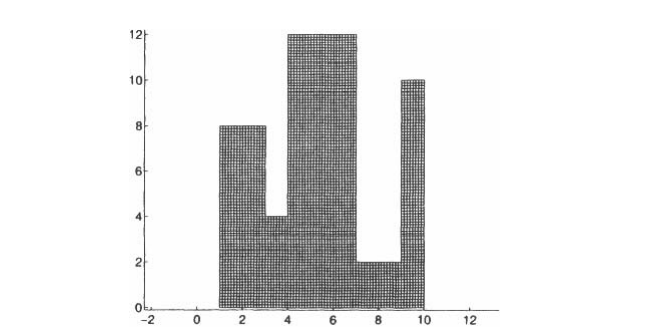
\includegraphics[width=0.9\linewidth]{9}
	\centering
	\label{pfig:ch13_8}
\end{figure}
\textbf{FIGURE 13.24:} A tessellation of a horizontally blocklike domain obtained using a program of 
Exercise 16 using the input data of part (b)(iii). There are 4694 nodes and 4432 rectangular 
elements.
\\
\textbf{Suggestions:} Part (a): First use the sort command to create a vector \texttt{cvals}  of the values of $c$ (in increasing order), with zero appended as the smallest value. Now find the minimum gaps occurring in the vectors \texttt{cvals}  and a. The inputted \texttt{sidelength}  should not be too small relative to the smaller of these two gaps. If the \texttt{sidelength} exceeds, say, twice this minimum gap value, have the function exit with an error flag (and no tessellation). Now move on to defining a vector $x$ for the vertical gridlines of the tessellation. Use a loop, running through each of the gaps determined from the values of a. If the size of a certain gap is less than twice the \texttt{sidelength}, let $x$ simply contain the values of a at the ends of this gap (no interior grid values); otherwise, use $k-1$ interior and equally spaced gridlines within the gap, where \texttt{k=cei l (gap/sidelength).}. (You need to verify that this will result in elements having horizontal sidelengths within the desired bounds.) In a similar fashion, define a vector $y$ for the horizontal gridlines of the tessellation. Next, use the vectors a, c, $x$, and $y$ to define the matrix \texttt{nodes}. This can be done with a double loop, but note that you will need to set it up so the larger $c$ value is used in cases where $x$ (i) lies on an interface of two blocks. Finally use the vectors $x, y$ and the matrix nodes to create the matrix \texttt{elems} of elements. You should set things up so that for a given element (row of the \texttt{elems} matrix) the nodes progress, say counterclockwise, around the element. With this being done, plotting of the tessellations (part (b)) can easily be accomplished using the following simple loop:
\\
\texttt{hold on, [el e2]=size(elems) ;
\\ 
for i=l:el
\\ 
R=nodes(elems(i, :) , :) ;
\\
xr=R(:,l); xr(5)=xr(1);yr=R(:,2); yr(5)=yr(1);
\\ 
plot (xr,yr)
\\
end }
\\
MATLAB's fin d command can be useful for many parts of this program.
	\item (a) Referring to Exercise 20, formulate the definition of the corresponding concept of a vertically blocklike domain.
	\\
(b) Write an M-file:
\\
$$\texttt{[x y node s eleras]=recttess\_vbd\_basic(a,c,sidelength )}$$ that will perform a basic rectangular tessellation of a vertically blocklike domain in a similar syntax and fashion to the program of part (a) of Exercise 16. Here, the input variable a is an increasing vector corresponding to the $y$-values of endpoints of the blocks, and the vector $c$ (length one less than $y$ ) gives the corresponding horizontal lengths of the blocks.
\\
(c) Run your program using the following sets of input variables:
\\
(i) $a=\left[\begin{array}{llllll}2 & 3 & 5 & 6 & 8&10\end{array}\right] c=\left[\begin{array}{lllll}6&8&7&4&2
\end{array}\right], h = 3,$
\\
(ii) $a=\left[\begin{array}{llllll}2 & 3 & 5 & 6 & 8&10\end{array}\right], c=\left[\begin{array}{lllll}6&8&7&4&2\end{array}\right], h=1$,
\\
(iii) $a=\left[\begin{array}{llllll}2 & 3 & 5 & 6 & 8&10\end{array}\right], c=\left[\begin{array}{lllll}6&8&7&4&2\end{array}\right], h=0.13$,
\\
\textbf{Suggesions:} Refer to those of Exercise 20 for ideas. If the reader has already completed Exercise 20 (a), the current program could invoke that of Exercise 20 along with a rotation of axes (viz. Section 7.2). After all, a vertically blocklike domain is simply a rotation of a horizontally blocklike domain and vice versa. The same goes for corresponding tessellations.
	\item Prove identity (5) equating the area of a triangle in the plane with vertices: $\left(x_{r}, y_{r}\right)$, $\left(x_{s}, y_{s}\right)$, and $\left(x_{t}, y_{t}\right)$ to half the absolute value of determinant of the matrix
$$
M=\left[\begin{array}{lll}
x_{r} & y_{r} & 1 \\
x_{s} & y_{s} & 1 \\
x_{t} & y_{t} & 1
\end{array}\right] .
$$
\texttt{Suggestion:} First use some properties of determinants from Chapter 7 to observe that the determinant will not change if a constant $X$ is added to all of the $x$-coordinates (first column) and/or a constant $Y$ is added to all the $y$-coordinates (second column). The corresponding effect on the triangle is simply a shift, leaving the area unchanged. Thus, we may assume that the triangle lies in the first quadrant. Furthermore, reduce to a configuration such as that shown in Figure 13.25. Express the area of the triangle shown as the difference of the sum of the areas of the two trapezoids between the top two edges of the triangle and the $x$-axis, less the area of the trapezoid between the bottom edge of the triangle and the $x$-axis. Compare this expression with the $\operatorname{det}(M)$. Recall that the area of a trapezoid with base $b$ and heights $h_{1}, h_{2}$ equals $(b / 2)\left(h_{1}+h_{2}\right)$.
\begin{figure}[H]
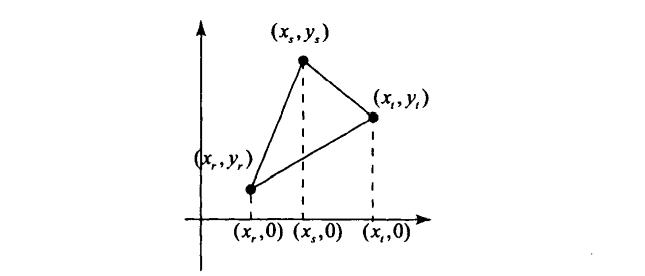
\includegraphics[width=0.9\linewidth]{10}
	\centering
	\label{pfig:ch13_8}
\end{figure}
\textbf{FIGURE 13.25:} Geometric diagram for the proof in Exercise 22. 
	\item To gain a deeper understanding of elements, it is often convenient to work with a so-called \textbf{standard element}, which is essentially equivalent to all elements. For our triangular elements, with three nodes at the vertices, we will use the standard element $\tilde{T}$ that has vertices $v_{1}=(1,0)$, $v_{2}=(0,1)$, \text { and } $v_{3}=(0,0)$ \text {. This standard element is illustrated in Figure 13.26. }
	\begin{figure}[H]
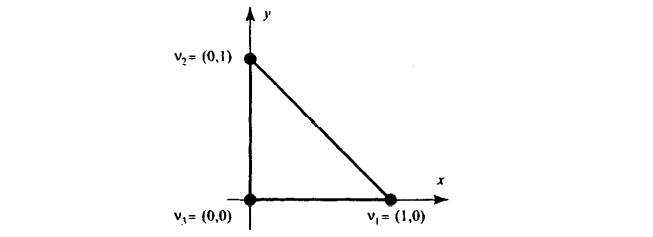
\includegraphics[width=0.9\linewidth]{11}
	\centering
	\label{pfig:ch13_8}
\end{figure}
\textbf{FIGURE 13.26:} Illustration of the standard element for all triangular elements with three nodes 
at the vertices
\\
\\
(a) Show that the standard local basis functions (viz. (7)) for the standard element of Figure $13.26$ are given by:
$$
\phi_{1}(x, y)=x, \phi_{2}(x, y)=y \text {, and } \phi_{3}(x, y)=1-x-y \text {. }
$$
(b) For any triangular element $T$ with specified vertices $v_{1}=\left(x_{r}, y_{r}\right), v_{2}=\left(x_{s}, y_{s}\right)$, and $v_{3}=\left(x_{t}, y_{t}\right)$ (labeled in counterclockwise order), show that the following affine mapping $(x, y)=F(\bar{x}, \bar{y})$ (see Section 7.2) will transform the standard basis element $\tilde{T}$ onto $T$ and map corresponding nodes onto one another:
$$
\begin{aligned}
&x=\left(x_{r}-x_{t}\right) \tilde{x}+\left(x_{s}-x_{t}\right) \tilde{y}+x_{t}, \\
&y=\left(y_{r}-y_{t}\right) \tilde{x}+\left(y_{s}-y_{t}\right) \tilde{y}+y_{t},
\end{aligned} \text { or }\left[\begin{array}{l}
x \\
y
\end{array}\right]=\left[\begin{array}{ll}
x_{r}-x_{t} & x_{s}-x_{t} \\
y_{r}-y_{t} & y_{s}-y_{t}
\end{array}\right]\left[\begin{array}{l}
\tilde{x} \\
\tilde{y}
\end{array}\right]+\left[\begin{array}{l}
x_{t} \\
y_{t}
\end{array}\right] .
$$
For clarity, we have used two different sets of coordinates, $(\tilde{x}, \tilde{y})$ for the coordinates of the plane for $\tilde{T}$ and $(x, y)$ for the coordinates of the plane of $T$. The action of this affine transformation is illustrated in Figure 13.27.
\begin{figure}[H]
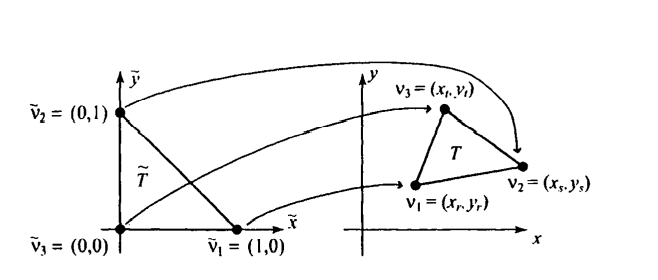
\includegraphics[width=0.9\linewidth]{12}
	\centering
	\label{pfig:ch13_8}
\end{figure}
\textbf{FIGURE 13.27:} Illustration of the action of the affine mapping of Exercise 23(b) that takes the 
standard element T onto an arbitrary element T. 
\\
\\
(c) Discover and then prove a relationship for the determinant of the $2 \times 2$ matrix of the affine transformation of part (b) and the areas of the two elements $T, \tilde{T}$. If you are not sure of the relationship, do some experiments using MATLAB. For the proof, cf., Exercise 22 .
\\
\\
(d) Writing $A=\left[\begin{array}{ll}x_{r}-x_{t} & x_{s}-x_{t} \\ y_{r}-y_{t} & y_{s}-y_{t}\end{array}\right]$ for the matrix of the affine transformation of part (b) observe first that the inverse affine mapping is given by: $(\tilde{x}, \tilde{y})=F^{-1}(x, y)=A^{-1} \cdot\left(\left[\begin{array}{l}x \\ y\end{array}\right]-\left[\begin{array}{l}x_{t} \\ y_{t}\end{array}\right]\right)$, and show that the standard local basis elements for $T$ are related to those (of part (a)) for $\tilde{T}$ as follows:
$$
\phi_{i}(x, y)=\vec{\phi}_{i}\left(F^{-1}(x, y)\right), i=1,2,3 .
$$
Note: Here we have used the notational convention of part (b), so that the $\tilde{\phi}_{i}$ 's are the standard local basis elements corresponding to $\bar{T}$, while $\phi$ are those corresponding to $T$. To prove this relation one simply needs to observe that both sides are linear functions of $(x, y)$ and compare them on the vertices $v_{1}, v_{2}, v_{3}$.
	\item (\textit{Quadratic Basis Functions on Triangular Elements}) For some BVPs it is desirable to use basis functions $\Psi_{j}$ which are piecewise quadratic rather than the piecewise linear basis functions that were used in the text. Thus, on each element $T$, such a basis function will have its general formula written as:
$$
\Psi_{j}(x, y)=a x^{2}+b x y+c y^{2}+d x+e y+f,
$$
where, in order to simplify notation, we have omitted subscripts and superscripts on the six coefficients $a, b, c, d, e, f$. Since we now have six local basis functions (for each term), we will need to correspondingly have six nodes on each element in order that the coefficients be uniquely determined. A very natural (and as it turns out effective) way to do this is to put three extra nodes on the midpoints of each of the edges of the elements. The corresponding standard element (see Exercise 23), is shown in Figure 13.28.
\begin{figure}[H]
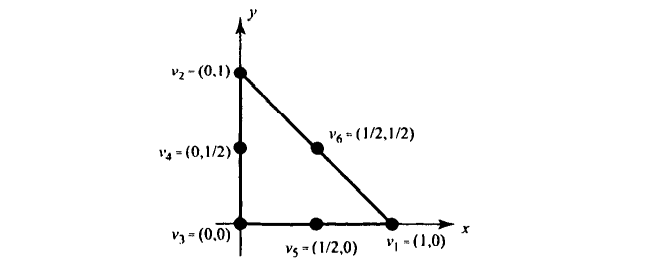
\includegraphics[width=0.9\linewidth]{13}
	\centering
	\label{pfig:ch13_8}
\end{figure}
\textbf{FIGURE 13.28:} The standard triangular element with six nodes for piecewise quadratic FEM. 
The three additional nodes from the piecewise linear standard elements are placed at the 
midpoints of the segments, the numbering is as before for the vertex nodes, while the midpoint 
nodes are numbered counterclockwise in order of the opposite vertices.
\\
\\
(a) Show that (by analogy with (7)) the corresponding standard local basis functions for the standard element of Figure $13.26$ are given by:
$$
\begin{aligned}
&\psi_{1}(x, y)=\phi_{1}(x, y) \cdot\left(2 \phi_{1}(x, y)-1\right), \\
&\psi_{2}(x, y)=\phi_{2}(x, y) \cdot\left(2 \phi_{1}(x, y)-1\right), \\
&\psi_{3}(x, y)=\phi_{3}(x, y) \cdot\left(2 \phi_{3}(x, y)-1\right) . \\
&\psi_{4}(x, y)=4 \phi_{2}(x, y) \cdot \phi_{3}(x, y), \\
&\psi_{5}(x, y)=4 \phi_{1}(x, y) \cdot \phi_{3}(x, y), \\
&\psi_{6}(x, y)=4 \phi_{1}(x, y) \cdot \phi_{2}(x, y),
\end{aligned}
$$
where the $\phi_{j}$ 's are the piecewise linear standard local basis functions of Exercise 23(a).
\\
(b) Do the six identities of part (a) continue to remain valid when the local basis functions correspond to an arbitrary element?
\\
(c) Show that the affine mapping $(x, y)=F(\tilde{x}, \tilde{y})$ of Exercise 23(b) maps the standard triangular element of Figure $13.28$ (viewed in the $\ddot{x} \tilde{y}$-plane) onto the corresponding triangular element with midpoint nodes (viewed in the $x y$-plane) such that the node correspondence is maintained.
\\
(d) Now letting $\bar{\psi}_{j}(x, y) j=1, \ldots, 6$, denote the standard local basis functions of part (a) and $\psi_{j}(x, y)$ denote the corresponding local basis functions for an arbitrary element, prove that $\psi_{i}(x, y)=\tilde{\psi}_{i}\left(F^{-1}(x, y)\right), i=1, \ldots, 6$, where $F$ is the affine mapping of part (c).
	\item (\textit{Quadratic Basis Functions on Triangular Elements, Cont.}) Let $\psi(x, y)=a x^{2}+b x y+c y^{2}$ $+d x+e y+f$ be a quadratic function on a triangular element $T$ with six nodes (vertices and midpoints). Assume that $\psi(x, y)=0$ on an entire line segment of $T$ that is opposite to vertex $v_{j}$. Prove that $\psi(x, y)$ can be factored as $\psi(x, y)=\phi_{j}(x, y) \cdot \phi(x, y)$ where $\phi_{j}(x, y)$ is the standard linear local basis function for the vertex $v_{j}$ and $\phi(x, y)$ is some other linear function $\phi(x, y)=a x+b y+c$.
\\
\textbf{Suggestion:} First prove this for the case of the standard element and $j=2$, then use affine mapping (see Exercises 23 and 24 ) to translate your proof to work for a general triangular element.
	\item (Quadratic Basis Functions on Triangular Elements, Cont.) (a) Use MATLAB to create threedimensional plots of each of the standard local basis functions $\psi_{j}(j=1, \ldots, 6)$ for the standard element of Figure 13.28. The graphs of two of these functions are roughly depicted in Figure 13.29.
	\\
\textbf{Suggestion:} One way to get high-resolution plots over such a triangular region is to triangulate it into much smaller elements and then use the \texttt{trimesh}.
\begin{figure}[H]
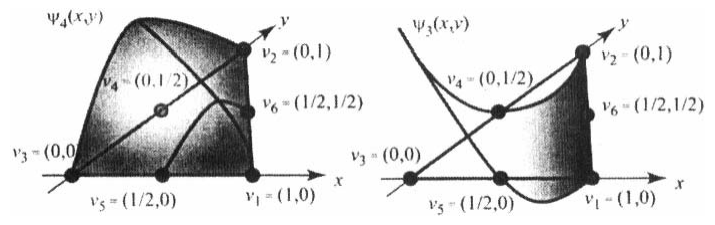
\includegraphics[width=0.9\linewidth]{14}
	\centering
	\label{pfig:ch13_8}
\end{figure}
\textbf{FIGURE 13.29:} Graphical illustration of two of the quadratic local basis functions for the 
standard triangular element of Figure 13.28. 
\\
\\
(b) Write down a formula for the (nonlocal) basis function $\Psi_{4}=\Psi_{4}(x, y)$ corresponding to the interior node $\$ 4$ of the triangulation of Figure $13.4$ using the nodal parameters given below Figure 13.5.
\\
\textbf{Suggestion:} The midpoint nodes will need to be numbered. This can be done systematically as in Example 13.1, but the linear systems will of course be larger.
\\
(c) Use MATLAB to plot the (nonlocal) basis function $\Psi_{4}=\Psi_{4}(x, y)$.
\\
(d) Repeat parts (b) and (c) for the midpoint node between the numbered nodes 4 and 5. 
	\item Given any finite set $P=\left\{p_{1}, p_{2}, \cdots, p_{n}\right\}$ of distinct points in the plane, show that each of the corresponding Voronoi boxes $V\left(p_{i}\right)$ is a convex set.
	\\
\textbf{Suggestion:} Observe that a Voronoi box is an intersection of half-planes.
	\item As mentioned in the text, when a triangulation is created for a given domain to use in the FEM, it is usually desirable to have the angles of each of the elements not get too small. In this exercise you will be creating an $M$-file that will be able to perform a check for this on a given triangulation and locate any "problem elements."
	\\
(a) Write an M-file, called \texttt{theta = minangle(v1, v2, v3)} whose three input variables $v1, v2, v3$ are $2 \times 1$ matrices giving the coordinates of the three vertices of a triangle in the $x y$-plane, and whose output theta is the smallest (interior) angle of this triangle, measured in degrees.
\\
(b) Write an M-file called \texttt{ theta = minanglemesh(x,y,tri ) } whose inputs are two vectors $x, y$ of the same size giving the coordinates of the nodes of a triangulation, and $t r i$, a 3 -column matrix having as its rows the node numbers of the elements in the triangulation. The output theta will be the minimum angle (measured in degrees) of any angle of any element of the triangulation. Run this program on the triangulations of Figure $13.5$ (with parameters given in the matrices $N$ and $T$ preceding Example 13.1), as well as each of the triangulations created in Examole $13.2$ of the unit disk.
\\
(c) Write an M-file called \texttt{[badelems, thetas] = minanglemesh (x, y, tri, tol)} that, along with the input variables of part (b), has the additional input variable tol that will be a positive number denoting the smallest desired angle (measured in degrees) to be tolerated in a triangulation. There are two output variables: \texttt{badelems}, which will give the element numbers (corresponding to row numbers of \texttt{tri} ) whose minimum angles are less than \texttt{tol}, and \texttt{thetas}, which is a vector of the same size as \texttt{badelems} gives the corresponding offending minimum angles of the bad elements. Additonally, a graphic will be produced that will graph only the elements corresponding to \texttt{badelems}. This will allow for appropriate measures to be taken to modify the triangulation, if necessary. Run this program on the triangulations of Figure $13.5$ (with parameters given in the matrices $N$ and $T$ preceding Example 13.1), as well as each of the triangulations created in Example $13.2$ of the unit disk, using three different values for \texttt{tol} for each: The first one chosen so that there are no offending elements, the second chosen so that there are a few offending elements (if possible), and the third chosen so there are a lot of offending elements.
\end{enumerate}
\section{ THE FINITE ELEMENT METHOD FOR ELLIPTIC PDE'S 
}
In this section we will present versions of the FEM for solving the following general type of BVP on a domain $\Omega \subset \mathbb{R}^{2}$
\begin{equation}
\left\{\begin{array}{lll}
(P D E) & -\nabla \cdot(p \nabla u)+qu=f & \text { on } \Omega \\
(BCs) & u=g & \text { on } \Gamma_{1}\\
&\vec{n} \cdot \nabla u+ru=h  & \text { on } \Gamma_{2}
\end{array}\right.
\end{equation}
The data functions: $p, q, f, g, r, h$ are allowed to be functions of $(x, y)$, defined on their respective indicated sets. The boundary $\partial \Omega$ is decomposed into the portions $\Gamma_{1}$ and $\Gamma_{2}, \quad \partial \Omega=\Gamma_{1} \cup \Gamma_{2}$. On the first portion $\Gamma_{1}$ there are Dirichlet boundary conditions $u=g$, and on the complementary portion $\Gamma_{2}$ we are assuming generalized Neumann boundary or Robin boundary conditions: $\vec{n} \cdot(p \nabla u)+r u=h$. Here $\vec{n}=\vec{n}(x, y)$ denotes the outward unit normal vector defined on the $\partial \Omega$, and $\nabla u=(\partial u / \partial x, \partial u / \partial y)$ is the gradient of $u(x, y)$. Thus, from multivariable calculus, the dot product $\vec{n} \cdot \nabla u(x, y)$ is just the partial derivative of $u$ in the direction of the outward pointing normal vector $\vec{n}=\vec{n}(x, y)$ at any point $(x, y)$ on the boundary. If $r(x, y) \equiv 0$, the $\mathrm{BCs}$ on $\Gamma_{2}$ generalize the usual Neumann boundary conditions. ${ }^{9}$ We allow for the possibility that either $\Gamma_{1}=\partial \Omega$ (so $\Gamma_{2}=\varnothing$ ) and the boundary conditions are purely of Dirichlet form, or that $\Gamma_{2}=\partial \Omega$ with boundary conditions being entirely of Robin form. The PDE in (10) is written in the so-called divergence form. This is the most general form for linear elliptic PDEs on which the standard FEM is applicable, and indeed this is the most general elliptic PDE to which MATLAB's symbolic toolbox is applicable. A great many elliptic boundary value problems can be expressed in the form (10). Sometimes, it will be convenient for us to write the PDE in (10) in expanded form:
$$
-\partial / \partial x\left[p u_{x}\right]-\partial / \partial y\left[p u_{y}\right]+q u=f \quad \text { on } \Omega
$$
The reason for the negative signs will become clear once the FEM is introduced. This PDE is the natural generalization to two space variables of the ODEs that were considered in Section 10.5. We begin by outlining the FEM for the BVP (10) in the case of purely Dirichlet boundary conditions (i.e., $\Gamma_{2}=\varnothing$ ). The FEM will look quite similar to the one-dimensional version presented in Section $10.5$. The proofs of the underlying results will not be included in this text. They share many common elements with the one-dimensional theory presented in Section $10.5$, but for technical reasons, the higher dimensional analogues require some more advanced mathematical machinery (including, for example, some elements of Sobolev spaces). The interested reader can consult one of the following references: [Cia-02], $[\mathrm{AxBa}-84],[\mathrm{StFi}-73]$, or [Joh-87] for more details on the theory.

In cases of purely Dirichlet boundary conditions and when the data the BVP (10) satisfy: $p, q, f$ are piecewise continuous on $\Omega$, along with the first partial
\footnotetext[9]{ Let us briefly review the physical significance of the three types of $\mathrm{BCs}$ in the context of a steadystate heat distribution BVP (a prototypical BVP). The Dirichlet boundary condition $u=g$ means that (on the portion of the boundary where the condition holds) the boundary is being maintained (by some coolant or heat reservoir) at a specified temperature. The Neumann boundary condition $\vec{n} \cdot \nabla u=0$ means that the boundary is insulated (no heat loss or transfer). The Robin boundary condition (after dividing through by $p$, which will always be assumed positive): $\vec{n} \cdot \nabla u+r u=h$ when written in the form $\vec{n} \cdot \nabla u=-r(u-\tilde{h})$ looks like the usual Newton's law of cooling where the net heat transfer (out of the region) is proportional to the difference of the inside temperature $(u)$ and the outside temperature $(\vec{h})$.}
derivatives of $p$ and $q, g$ is piecewise continuous on $\partial \Omega$ and $p(x, y)>0, q(x, y) \geq 0$, the BVP can be shown to be equivalent to the minimization problem:
\\
\\
Minimize the functional:
\begin{equation}
F[u]=\iint_{\Omega}\left[\frac{1}{2} p u_{x}^{2}+\frac{1}{2} p u_{y}^{2}+\frac{1}{2} q u^{2}-f u\right] d x d y
\end{equation}
over the following set of admissible functions:
\begin{center}
$\mathcal{A}=\left\{v: \Omega \rightarrow \mathbb{R}: v(x)\right.$ is continuous, $v^{\prime}(x)$ is piecewise continuous
\\ and bounded, and $v(x, y)=g(x, y)$ on $\partial \Omega\}$.
\end{center}
The concept of piecewise continuity on $\Omega$ (or $\partial \Omega$ ) simply means that the domain (or boundary) can be broken up into finitely many elements (arcs) on each of which the given function reduces to a continuous function.
\\
\\
Analogous to the one-dimensional method presented in Section 10.5, the FEM will solve a corresponding finite-dimensional minimization problem where the functional $F[u]$ of $(11)$ is kept the same, but the set of admissible functions is reduced to an approximating smaller set that is determined by the basis functions of the triangulation. Thus we will be looking for minimizers of the functional $F$ among functions of the form $v=\sum_{i=1}^{m} c_{i} \Phi_{i}$, where the $\Phi_{i}=\Phi_{i}(x, y)$ are the basis functions. The basis functions corresponding to nodes on the boundary will have their coefficients determined by the Dirichlet boundary conditions; it is the remaining coefficients (corresponding to interior nodes) that need to be We follow this outline with some additional details and then give examples.
\\
\\
\textbf{FEM FOR THE BVP (10) IN CASE OF PURELY DIRICHLET BC'S $\left(\Gamma_{2}=\varnothing\right):$
\\
\\ 
Step $\#1$: Decompose the domain into elements, and represent the set of nodes and elements using matrices. Separate the nodes $N_{i}$ into the internal nodes:
\\
$N_{1}, N_{2}, \cdots, N_{n}$ (that lie in $\Omega$.), and the boundary nodes $N_{n+1}, N_{n+2}$, $\cdots, N_{m}$ (that lie on $\partial \Omega$ ). Denote the basis function $\Phi_{N_{i}}$ corresponding to node $N_{i}$ simply by $\Phi_{i}$.
\\
Step $\#2$: Use the Dirichlet BCs $u(x, y)=g(x, y)$ on $\partial \Omega$ to determine the coefficients of the boundary node basis functions of an admissible function:
\\
$v=\sum_{i=1}^{m} c_{i} \Phi_{i}$, i.e., $c_{i}=g\left(N_{i}\right)$ for each $i=n+1, n+2, \cdots, m$.
\\
Step $\#3$: Assemble the $n \times n$ stiffness matrix $A$ and load vector $b$ needed to determine the remaining coefficients $c_{1}, c_{2}, \cdots, c_{n}$ that work to solve the discrete minimization problem corresponding to the BVP.
\\
Step $\#4$: Solve the stiffness equation $A c=b$, and obtain the FEM solution $$v=\sum_{i=1}^{m} c_{i} \Phi_{i}$$}
The first step was examined in detail in the last section for triangular elements with piecewise linear basis functions. Such elements and basis functions are the ones that will be used exclusively in the text of this section. The exercises will consider some other sorts of elements and/or basis functions. Step $\# 2$ is rather clear. Step $\#3$ will be accomplished by a so-called \textbf{assembly} technique where the entries of the stiffness matrix and load vectors are built by looking at the contributions of each element.
\\
\\
If we substitute the expression $v=\sum_{i=1}^{m} c_{i} \Phi_{i}$ for $u$ into the functional $F[u]$, and then differentiate with respect to $c_{k}$ (under the integral sign), we arrive at the following equation (Exercise 17):
\begin{equation}
\begin{aligned}
\frac{\partial}{\partial c_{k}} F\left[\sum_{i=1}^{m} c_{i} \Phi_{i}\right]=\iint_{\Omega}\left[p \sum_{i=1}^{m} c_{i} \partial_{x}\left(\Phi_{i}\right) \partial_{x}\left(\Phi_{k}\right)\right.&+p \sum_{i=1}^{m} c_{i} \partial_{y}\left(\Phi_{i}\right) \partial_{y}\left(\Phi_{k}\right) \\
&\left.+q \sum_{i=1}^{m} c_{i} \Phi_{i} \Phi_{k}-f \Phi_{k}\right] d x d y
\end{aligned}
\end{equation}
Keeping in mind that the values of $c_{k}$ for $k>n$ will have been computed in Step $\#2$, since we seek a critical point of $F$, we set the above equations equal to zero for $1 \leq k \leq n$ to obtain the following $n \times n$ linear system for the unknown coefficients:
\begin{equation}
A c=b,
\end{equation}
where the $c$ represents the (column) vector of the unknown (internal node) coefficients:
\begin{equation}
c=\left[\begin{array}{llll}c_{1} & c_{2} & \cdots & c_{n}\end{array}\right]^{\prime}.
\end{equation}
 The entries of the stiffness matrix $A=\left[\begin{array}{l}a_{i j}\end{array}\right]$ are given by (Exercise 17):
\begin{equation}
a_{i j}=\iint_{\Omega}\left[p \nabla \Phi_{i} \cdot \nabla \Phi_{j}+q \Phi_{i} \Phi_{j}\right] d x d y \quad(1 \leq i, j \leq n)
\end{equation}
and the entries of the load vector $b=\left[b_{j}\right]$ are given by:
\begin{equation}
b_{j}=\iint_{\Omega} f \Phi_{j} d x d y-\sum_{s=n+1}^{m} \iiint_{\Omega}\left[p \nabla \Phi_{s} \cdot \nabla \Phi_{j}+q \Phi_{s} \Phi_{j}\right] d x d y(1 \leq j \leq n) .
\end{equation}
We point out that the coefficients $c_{s}(s>n)$ are known from Step $\#2$. Note that from (15) (since the dot product is commutative: $\vec{v} \cdot \vec{w}=\vec{w} \cdot \vec{v}$ ) it follows that $a_{i j}=a_{j i}$, i.e., the stiffness matrix is a symmetric matrix.
\\

Keeping in mind that each of the basis functions is made up of its linear "pieces" on each of the elements, it is more efficient to compute the stiffness entries $a_{i j}$ and load entries $b_{j}$ by running through each of the elements and adding up contributions. Assuming that the nodes and elements have been stored in a 2column matrix $N$ and a 3 -column matrix $E$, respectively (as in the last section, but then we labeled the element matrix as $T$ ), we now outline the assembly process:
\\
\\
\textbf{ASSEMBLY PROCESS FOR THE FEM FOR (10) IN CASE OF PURELY DIRICHELT BC'S $\left(\Gamma_{2}=\varnothing\right)$ :
\\
\\
Step $\#1$: Initialize $n \times n$ stiffness matrix $A$ and $n \times 1$ load vector $b$ with all zero entries.
\\
Step $\#2$: Let $\ell$ run from 1 to $L=$ the number of elements ( $=$ number of rows of the matrix $E$ whose $\ell$ th row gives the node numbers of the $\ell$ th element $T_{l}$ ). For each index $\ell$, we create the $3 \times 3$ element stiffness matrix $A^{l}=\left[a_{a \beta}^{l}\right]$ $\left(1 \leq \alpha, \beta \leq 3\right.$ ) for the element $T_{\ell}$ and the corresponding $3 \times 1$ element load vector $b^{l}=\left\{b_{a}^{\ell} \mid\right.$ by restricting the integrals in formulas (15) and (16) from $\Omega$ to $T_{\ell}$ :
\begin{equation}
a_{\alpha \beta}^{l}=\iint_{T_{i}}\left[p \nabla \Phi_{i_{\varepsilon}} \cdot \nabla \Phi_{i_{p}}+q \Phi_{i_{\xi}} \Phi_{i_{\rho}} \mid d x d y \quad(1 \leq \alpha, \beta \leq 3),\right.
\end{equation}
and
\begin{equation}
b_{\alpha}^{\prime}=\iint_{T_{t}} f \Phi_{i_{e}} d x d y-\sum_{s=n+1}^{m} c_{s} \iint_{T_{t}}\left[p \nabla \Phi_{s} \cdot \nabla \Phi_{i_{e}}+q \Phi_{s} \Phi_{i_{e}} \mid d x d y \quad(1 \leq \alpha \leq 3)\right.
\end{equation}
(Here, the index $i_{\alpha}$ denotes the global node number corresponding to the $\alpha$ th vertex of $T_{\ell}$, i.e., $i_{\alpha}=E(\ell, \alpha)$, whereas the local node number $\alpha$ for a vertex of $T_{\ell}$ is just the corresponding column number of the index $\alpha$ in the $\ell$ th row of the element matrix $E$.) We then transplant these contributions into the appropriate places of the (global) stiffness matrix and load vector:
\begin{equation}
A(E(\ell, \alpha), E(\ell, \beta))=A(E(\ell, \alpha), E(\ell, \beta))+a_{\alpha \beta}^{\ell}(1 \leq \alpha, \beta \leq 3) \\
\end{equation}
\text { and }
\begin{equation}
b(E(\ell, \alpha))=\bar{b}(\bar{E}(\bar{\ell}, \alpha))+\dot{b}_{\alpha}^{\ell}(1 \leq \alpha \leq 3)
\end{equation}}
We point out that formulas $\left(15^{\prime}\right)$ and $\left(16^{\prime}\right)$ need only be carried out when the indices $\alpha$ and/or $\beta$ correspond to interior nodes.. ${ }^{10}$\footnotetext[10]{ Otherwise the entries are meaningless. Thus, technically, the clement stiffness matrices $A^{\prime}$ (load vectors $b^{t}$ ) will not be complete $3 \times 3(3 \times 1)$ matrices in cases where the element $T_{t}$ has some of its vertices on the boundary (in Example 13.5, this will be the case for all of the elements).} Also, the integrands in summation of $\left(16^{\prime}\right)$ will vanish on the element $T$, unless the corresponding exterior node (number $s$ ) is a vertex of $T_{\ell}$.
\\
\\
We turn now to a simple example involving the Poisson PDE and constant (Dirichlet) boundary conditions on the hexagonal domain of the last section with only eight triangular elements (Figure 13.5). MATLAB will be able to help us with general multiple integrals, and we will explain how this can be done after this introductory example. The integrals that will need to get done in the course of this example will be simple enough to do by hand, and all will be evaluated using the results of the following exercise for the reader:
\\
\\
EXERCISE FOR THE READER 13.5: Let $T$ denote any (convex) triangle in the plane having vertices $v_{1}=\left(x_{r}, y_{r}\right), v_{2}=\left(x_{s}, y_{s}\right)$, and $v_{3}=\left(x_{t}, y_{t}\right)$ (Figure 13.30), and let $\phi=\phi_{3}$ denote the local basis function for $T$ corresponding to the vertex $v_{3}$, i.e., $\phi(x, y)$ is the linear function determined by the equations $\phi\left(v_{i}\right)=\delta_{i 3}$ $(i=1,2,3)$. Establish the following formulas:
\\
(a) The gradient vector $\vec{\nabla} \phi$ points in the direction of the altitude $\vec{a}$ and has magnitude $\|\nabla \phi\|=1 /\|\vec{a}\|$.
\\
(b) $\iint_{T} \phi(x, y) d x d y=\frac{1}{3} \operatorname{Area}(T)$.
\begin{figure}[H]
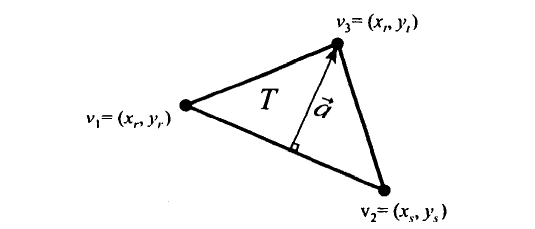
\includegraphics[width=0.9\linewidth]{15}
	\centering
	\label{pfig:ch13_8}
\end{figure}
\textbf{FIGURE 13.30:} A typical (convex) triangular element whose local basis function $\phi=\phi_{3}$ 
is analyzed in Exercise for the Reader 13.5. Since the element is convex, the (blue) altitude 
vector $\vec{a}$ shown will lie inside the triangle. 
\\
\\
\textbf{EXAMPLE 13.5:} Let $\Omega$ be the hexagonal domain of Figure 13.5 with eight nodes (as labeled) given by: $\#1$: $(1,1), \#2:(2.5,1), \#3:(0,0), \#4:(1,0)$, $\#5$:
$(2.5,0)$, $\#6$: $(3.5,0), \# 7:(1,-1)$, and $\#8$: $(2.5,-1)$. Consider the following Poisson BVP for this domain:
$$
\left\{\begin{array}{lrlrl}
(\mathrm{PDE}) & -\Delta u & =f(x, y) & & \text { on } \Omega \\
(\mathrm{BC}) & u & =1 & & \text { on } \partial \Omega
\end{array},\right.
$$
where the "load" $f(x, y)$, is given by:
$$
f(x, y)= \begin{cases}0, & \text { if } x \leq 2.5, \\ -1, & \text { if } x>2.5\end{cases}
$$
Using the triangulation of Figure $13.5$ and the corresponding piecewise linear basis functions of the last section, apply the FEM to solve this BVP.
\\
\\
SOLUTION: In this problem the BC is purely Dirichlet, so we may follow the above procedure.
\\
\\
The numbering of the nodes in Figure $13.5$ has one drawback in that it does not conform to our current notation where the interior nodes are numbered first. We could redo the numbering to conform but instead will work around the numbering that was already set up. The corresponding matrices $N$ (odes) and $E$ (lements) are reproduced here:
$$
N=\left[\begin{array}{cc}
1 & 1 \\
2.5 & 1 \\
0 & 0 \\
1 & 0 \\
2.5 & 0 \\
3.5 & 0 \\
1 & -1 \\
2.5 & -1
\end{array}\right], \quad E=\left[\begin{array}{lll}
1 & 3 & 4 \\
1 & 2 & 4 \\
2 & 4 & 5 \\
2 & 5 & 6 \\
3 & 4 & 7 \\
4 & 5 & 7 \\
5 & 7 & 8 \\
5 & 6 & 8
\end{array}\right]
$$
Keep in mind that there are $m=8$ nodes here of which $n=2$ are interior (nodes $\# 4$ and $\# 5$ ). Thus an admissible function (for the FEM) $v=\sum_{i=1}^{8} c_{i} \Phi_{i}$ will have all but two of the coefficients $\left(c_{4}, c_{3}\right)$ determined by the Dirichlet boundary conditions. Since (in the notation of $(10)) g(x, y)=1$, we have that $c_{i}=g\left(N_{i}\right)=1$ for $i \neq 4,5$, and so the FEM solution will have form: $v=c_{4} \Phi_{4}+c_{5} \Phi_{5}+\sum_{s \neq 4,5} \Phi_{s}$ and the rest of the problem is to compute these remaining two coefficients.
\\
\\
We are now at the assembly stage of the FEM. Note that since (in the notation of $(10)), p=1$ and $q=0$, and $c_{s}=g\left(N_{s}\right)=1(s \neq 4,5)$, equations $\left(15^{l}\right)$ and $\left(16^{l}\right)$ simplify to:
$$
a_{\alpha \beta}^{\ell}=\iint_{T_{\ell}} \nabla \Phi_{i_{a}} \cdot \nabla \Phi_{i_{\beta}} d x d y \quad(1 \leq \alpha, \beta \leq 3)
$$
and
$$
b_{\alpha}^{\ell}=\iint_{T_{t}} f \Phi_{i_{o}} d x d y-\sum_{s \neq 4, S} \iint_{T_{t}} \nabla \Phi_{s} \cdot \nabla \Phi_{i_{a}} d x d y(1 \leq \alpha \leq 3),
$$
respectively (we have incorporated the change needed to accommodate the node numbering scheme).
\\
\\
We initialize a $2 \times 2$ stiffness matrix $A$ of zeros and the corresponding $2 \times 1$ initial load vector $b$ and pass now to a detailed calculation of the first iteration of the assembly loop: $\ell=1$ corresponding to the first element $T_{1}$ of Figure 13.5. Figure $13.31$ shows this element and its corresponding element stiffness matrix $A^{\prime}$.
\begin{figure}[H]
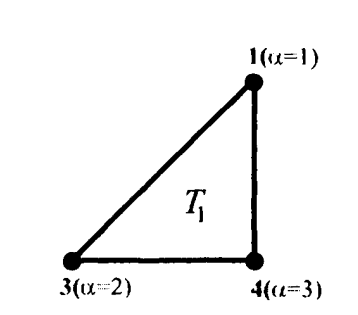
\includegraphics[width=0.3\linewidth]{16}
	\centering
	\label{pfig:ch13_8}
\end{figure}
$$
\begin{aligned}
&A^{2}=\left[\begin{array}{lll}
a_{11}^{1} & a_{12}^{1} & a_{13}^{1} \\
a_{21}^{1} & a_{22}^{1} & a_{23}^{1} \\
a_{31}^{1} & a_{32}^{1} & a_{33}^{1}
\end{array}\right] \begin{array}{lll}
\leftarrow N_{2}\\
\leftarrow N_{2}\\
\leftarrow N_{2}
\end{array}
\\
&\begin{array}{ccccc}
~&~&~\uparrow &~\uparrow &~\uparrow\\
~&~&~N_{1}&~N_{2}&~N_{4}
\end{array}
\end{aligned}
$$
\textbf{FIGURE 13.31:} (a) (left) Illustration of the first element $T_{1}$ of Figure $13.5$ with the global node numbers (from Figure 13.5) as well as the local node numbers from the matrix $T$. (b) (right) The corresponding element stiffness matrix $A^{\prime}$ along with a labeling of the corresponding nodes.
\\
Of the nodes for $T_{1}$, only node $\# 4(\alpha=3)$ is an interior node so we need only compute the single entry:
$$
a_{33}^{1}=\iint_{T_{1}} \nabla \Phi_{4} \cdot \nabla \Phi_{4} d x d y
$$
From the formula obtained in Example $13.1$ for $\Phi_{4}$, we know that on $T_{1}$, $\Phi_{4}(x, y)=x-y$, so that $\nabla \Phi_{4}=(1,-1)$ (this also follows from the preceding exercise for the reader), and $\nabla \Phi_{4} \cdot \nabla \Phi_{4}=2$. Consequently,
$$
a_{33}^{1}=\iint_{T_{1}} \nabla \Phi_{4} \cdot \nabla \Phi_{4} d x d y=\iint_{T_{1}} 2 d x d y=2 \cdot \operatorname{Area}\left(T_{1}\right)=2 \cdot(1 / 2)=1 .
$$
Similarly, we have only to compute the single load entry:
\\
$$
b_{3}^{1}=\iint_{T_{1}} f \Phi_{4} d x d y-\sum_{x=1,3} \iint_{T_{1}} \nabla \Phi_{5} \cdot \nabla \Phi_{4} d x d y
$$
Since the load $f(x, y)$ vanishes throughout $T^{1}$, only the latter two integrals need to be computed. Both integrands are constants and so the integrals can be simply evaluated as the preceding one. We need the gradients of $\Phi_{1}$ and of $\Phi_{3}$ on $T^{1}$. Using part (a) of the preceding exercise for the reader, we compute $\nabla \Phi_{1}=(0,1)$ and $\nabla \Phi_{3}=(-1,0)$ and so the corresponding dot products with $\nabla \Phi_{4}=(1,-1)$ are both $-1$. Hence,
$$
b_{3}^{1}=-\iint_{T_{1}} \nabla \Phi_{1} \cdot \nabla \Phi_{4} d x d y-\iint_{T_{1}} \nabla \Phi_{3} \cdot \nabla \Phi_{4} d x d y=-\left(-\operatorname{Area}\left(T_{1}\right)-\operatorname{Area}\left(T_{1}\right)\right)=1
$$
The just-computed entries $a_{33}^{1}=1, b_{3}^{1}=1$ need to be transplanted to update the appropriate entries of the stiffness matrix and load vector $b$ :
$$
\begin{aligned}
&A=\left[\begin{array}{ll}
a_{11} & a_{12}\\
a_{21}& a_{22}
\end{array}\right] \begin{array}{lll}
\leftarrow N_{4}\\
\leftarrow N_{5}
\end{array}
\\
&\begin{array}{cccc}
~&~&~\uparrow &~\uparrow\\
~&~&~N_{4}&~N_{4}
\end{array}
\end{aligned}
$$
\\
$$
b=\left[\begin{array}{l}
b_{1} \\
b_{2}
\end{array}\right]\begin{array}{ll}
\leftarrow N_{4}\\
\leftarrow N_{5}
\end{array}
$$
Since the local index $\alpha=3$ corresponds to the internal node $N_{4}$, the corresponding index for the (global) stiffness matrix and load vector is 1 , and we update: $a_{11}=a_{11}+a_{33}^{1}=0+1=1$, and $b_{1}=b_{1}+b_{3}^{1}=0+1=1$. In summary, after the first iteration of the assembly process $(\ell=1)$, our updated stiffness matrix and load vector are as follows:
$$
A=\left[\begin{array}{ll}
1 & 0 \\
0 & 0
\end{array}\right], \quad b=\left[\begin{array}{l}
1 \\
0
\end{array}\right]
$$
The treatment for the next iteration $\ell=2$ is quite similar since the element $T_{2}$ also has one interior node ($\#4$) and two boundary nodes ($\#1, \#2$). To prepare for the computations, we note that $\operatorname{Area}\left(T_{2}\right)=3 / 4$ and on $T_{2}$ :
$$
\nabla \Phi_{1}=(-2 / 3,1), \quad \nabla \Phi_{2}=(2 / 3,0), \quad \nabla \Phi_{4}=(0,-1)
$$
We have used Exercise for the Reader 13.5. Actually, with less work, the needed gradient vectors here and in all other computations of this example can be gleaned from the explicit formula for $\Phi_{4}$ obtained in Example $13.1$ by comparing relevant triangles.
\\
\\
From the second row of the element matrix $E$, we see that the three vertices of $T_{2}$, nodes $\#1, \#2$, and $\#4$, have local node numbers $\alpha=1,2$, and 3 , respectively, so that the node correspondence for the element stiffness matrix $A^{2}$ is as follows:
\\
$$
\begin{aligned}
&A^{2}=\left[\begin{array}{lll}
a_{11}^{2} & a_{12}^{2} & a_{13}^{2} \\
a_{21}^{2} & a_{22}^{2} & a_{23}^{2} \\
a_{31}^{2} & a_{32}^{2} & a_{33}^{2}
\end{array}\right] \begin{array}{lll}
\leftarrow N_{2}\\
\leftarrow N_{2}\\
\leftarrow N_{2}
\end{array}
\\
&\begin{array}{ccccc}
~&~&~\uparrow &~\uparrow &~\uparrow\\
~&~&~N_{1}&~N_{2}&~N_{4}
\end{array}
\end{aligned}
$$
Since only node $N_{4}$ is internal, we need only compute the entry $a_{33}^{2}$ and the corresponding element load vector entry $b_{3}^{2}$, and since $f(x, y)$ again vanishes on $T_{2}$, these computations can be carried out just as before, using the above gradients and area:
$$
\begin{gathered}
a_{33}^{2}=\iint_{T_{2}} \nabla \Phi_{4} \cdot \nabla \Phi_{4} d x d y=\iint_{T_{2}} 1 d x d y=\operatorname{Area}\left(\mathrm{T}_{2}\right)=3 / 4, \\
b_{3}^{2}=-\iint_{T_{2}} \nabla \Phi_{1} \cdot \nabla \Phi_{4} d x d y-\iint_{T_{2}} \nabla \Phi_{2} \cdot \nabla \Phi_{4} d x d y=-\left(-\operatorname{Area}\left(T_{2}\right)+0\right)=3 / 4 .
\end{gathered}
$$
Transplanting these results into the appropriate places in the stiffness matrix and load vector results in the following updates:
$$
A=\left[\begin{array}{cc}
1+3 / 4 & 0 \\
0 & 0
\end{array}\right]=\left[\begin{array}{cc}
7 / 4 & 0 \\
0 & 0
\end{array}\right], \quad b=\left[\begin{array}{c}
1+3 / 4 \\
0
\end{array}\right]=\left[\begin{array}{c}
7 / 4 \\
0
\end{array}\right]
$$
Proceeding now to $\ell=3$, the situation is a bit different in that the element $T_{3}$ has two internal nodes. This will mean that we will need to compute a total of six entries (four for the element stiffness matrix $A^{3}$ and two for the corresponding element load vector $\left.b^{3}\right)$. We obtain, as before, the area $\operatorname{Area}\left(T_{3}\right)=3 / 4$, and the gradient vectors on $T_{3}$,
$$
\nabla \Phi_{2}=(0,1), \quad \nabla \Phi_{4}=(-2 / 3,0), \quad \nabla \Phi_{5}=(2 / 3,-1)
$$
From the third row of the element matrix $E$, we see that the three vertices of $T_{3}$ : nodes $\#2, \#4, and \#5$ have local node numbers $\alpha=1,2$, and 3 , respectively, so that the node correspondence for the element stiffness matrix $A^{3}$ is as follows:
$$
\begin{aligned}
&A^{2}=\left[\begin{array}{lll}
a_{11}^{3} & a_{12}^{3} & a_{13}^{3} \\
a_{21}^{3} & a_{22}^{3} & a_{23}^{3} \\
a_{31}^{3} & a_{32}^{3} & a_{33}^{3}
\end{array}\right] \begin{array}{lll}
\leftarrow N_{2}\\
\leftarrow N_{4}\\
\leftarrow N_{5}
\end{array}
\\
&\begin{array}{ccccc}
~&~&~\uparrow &~\uparrow &~\uparrow\\
~&~&~N_{2}&~N_{4}&~N_{5}
\end{array}
\end{aligned}
$$
The computations of the needed entries of $A^{3}$ and $b^{3}$ are now done just as before. We briefly summarize them:
$$
\begin{aligned}
&a_{22}^{3}=\iint_{T_{3}} \nabla \Phi_{4} \cdot \nabla \Phi_{4} d x d y=\frac{4}{9} \cdot \frac{3}{4}=1 / 3, \quad a_{23}^{3}=a_{32}^{3}=\iint_{T_{3}} \nabla \Phi_{4} \cdot \nabla \Phi_{5} d x d y=-\frac{4}{9} \cdot \frac{3}{4}=-1 / 3 \\
&\qquad a_{33}^{3}=\iint_{T_{3}} \nabla \Phi_{5} \cdot \nabla \Phi_{5} d x d y=\frac{13}{9} \cdot \frac{3}{4}=13 / 12, \quad b_{2}^{3}=-\iint_{T_{3}} \nabla \Phi_{2} \cdot \nabla \Phi_{4} d x d y=0
\end{aligned}
$$
\begin{flushleft}
$and ~b_{3}^{3}=-\iint_{T_{3}} \nabla \Phi_{2} \cdot \nabla \Phi_{5} d x d y=-\left(-\operatorname{Area}\left(T_{3}\right)\right)=3 / 4$
\end{flushleft}
Transplanting these results into the appropriate places in the stiffness matrix and load vector results in the following updates:
$$
A=\left[\begin{array}{cc}
7 / 4+1 / 3 & 0-1 / 3 \\
0-1 / 3 & 0+13 / 12
\end{array}\right]=\left[\begin{array}{cc}
25 / 12 & -1 / 3 \\
-1 / 3 & 13 / 12
\end{array}\right], \quad b=\left[\begin{array}{l}
7 / 4+0 \\
0+3 / 4
\end{array}\right]=\left[\begin{array}{l}
7 / 4 \\
3 / 4
\end{array}\right]
$$
In the next iteration, $\ell=4$ and $f(x, y)$ no longer vanishes on the element. Since $f(x, y)$ is constant throughout $T_{4}$, however, we will still be able to use Exercise for the Reader $13.5$ to evaluate the new integral that arises. The nodes of $T_{4}$ : $N_{2}, N_{5}, N_{6}$ have local node numbers (from the fourth row of $E$ ) $\alpha=1,2,3$, respectively. The needed element area is $\operatorname{Area}\left(T_{4}\right)=1 / 2$, and the gradient vectors on $T_{4}$ :
$$
\nabla \Phi_{2}=(0,1), \quad \nabla \Phi_{\mathrm{5}}=(-1,-1), \quad \nabla \Phi_{\mathrm{6}}=(1,0) .
$$
As only one of the nodes is internal, we have only two entries to compute:
$$
\begin{gathered}
a_{22}^{4}=\iint_{T_{4}} \nabla \Phi_{5} \cdot \nabla \Phi_{5} d x d y=\iint_{T_{2}} 2 d x d y=1, \quad \text { and } \\
b_{2}^{4}=\iint_{T_{4}} f \Phi_{5} d x d y-\iint_{T_{4}} \nabla \Phi_{2} \cdot \nabla \Phi_{5} d x d y-\iint_{T_{4}} \nabla \Phi_{6} \cdot \nabla \Phi_{5} d x d y \\
=-\frac{1}{3} \operatorname{Area}\left(T_{4}\right)-\left(-\operatorname{Area}\left(T_{4}\right)-\operatorname{Area}\left(T_{4}\right)\right)=5 / 6 .
\end{gathered}
$$
(In the last calculation we use Exercise for the Reader 13.5(b).) The updated stiffness matrix and load vectors now become:
\\
$$
A=\left[\begin{array}{cc}
25 / 12 & -1 / 3 \\
-1 / 3 & 13 / 12+1
\end{array}\right]=\left[\begin{array}{cc}
25 / 12 & -1 / 3 \\
-1 / 3 & 25 / 12
\end{array}\right], \quad b=\left[\begin{array}{c}
7 / 4 \\
3 / 4+5 / 6
\end{array}\right]=\left[\begin{array}{c}
7 / 4 \\
19 / 12
\end{array}\right]
$$
Each of the remaining four iterations is done almost identically to one of the four that has just been done. We summarize each remaining iteration only by the stiffness matrix and load vector updates:
\\
$$
\begin{aligned}
&\ell=5: \quad A=\left[\begin{array}{cc}
25 / 12+1 & -1 / 3 \\
-1 / 3 & 25 / 12
\end{array}\right]=\left[\begin{array}{cc}
37 / 12 & -1 / 3 \\
-1 / 3 & 25 / 12
\end{array}\right], \quad b=\left[\begin{array}{c}
7 / 4+1 \\
19 / 12
\end{array}\right]=\left[\begin{array}{c}
11 / 4 \\
19 / 12
\end{array}\right] \\
&\ell=6: \\
&A=\left[\begin{array}{cc}
37 / 12+13 / 12 & -1 / 3-1 / 3 \\
-1 / 3-1 / 3 & 25 / 12+1 / 3
\end{array}\right]=\left[\begin{array}{cc}
25 / 6 & -2 / 3 \\
-2 / 3 & 29 / 12
\end{array}\right], b=\left[\begin{array}{c}
11 / 4+3 / 4 \\
19 / 12
\end{array}\right]=\left[\begin{array}{c}
15 / 4 \\
19 / 12
\end{array}\right] \\
&\ell=7: A=\left[\begin{array}{cc}
25 / 6 & -2 / 3 \\
-2 / 3 & 29 / 12+3 / 4
\end{array}\right]=\left[\begin{array}{cc}
25 / 6 & -2 / 3 \\
-2 / 3 & 19 / 6
\end{array}\right], \quad b=\left[\begin{array}{c}
15 / 4 \\
19 / 12+3 / 4
\end{array}\right]=\left[\begin{array}{c}
15 / 4 \\
7 / 3
\end{array}\right]
\end{aligned}
$$
and finally,
\\
$$
\ell=8: \quad A=\left[\begin{array}{cc}
25 / 6 & -2 / 3 \\
-2 / 3 & 19 / 6+1
\end{array}\right]=\left[\begin{array}{cc}
25 / 6 & -2 / 3 \\
-2 / 3 & 25 / 6
\end{array}\right], \quad b=\left[\begin{array}{c}
15 / 4 \\
7 / 3+5 / 6
\end{array}\right]=\left[\begin{array}{l}
15 / 4 \\
19 / 6
\end{array}\right]\\
$$
\\
With the stiffness matrix and load vector now "assembled," the remaining coefficients $c_{4}, c_{5}$ are simply the solutions of the linear system:
$$
A c=b \Leftrightarrow\left[\begin{array}{ll}
25 / 6 & -2 / 3 \\
-2 / 3 & 25 / 6
\end{array}\right]\left[\begin{array}{l}
c_{4} \\
c_{5}
\end{array}\right]=\left[\begin{array}{l}
15 / 4 \\
19 / 6
\end{array}\right] \Rightarrow\left[\begin{array}{l}
c_{4} \\
c_{5}
\end{array}\right]=\left[\begin{array}{c}
1277 / 1218 \\
565 / 609
\end{array}\right]
$$
With this small system (solved on MATLAB) exact arithmetic was feasible. The FEM solution $v=c_{4} \Phi_{4}+c_{5} \Phi_{3}$ can now be plotted quite easily using the trimesh command as in the last section. We need to make sure we have the node matrix $N$ and the element matrix $E$ stored, and then assign the values for $c_{4}, c_{5}$ to nodes $\#4$, $\#5$ and values of one for the remaining nodes (from the Dirichlet BCs):
\\
\texttt{>> N=[l 1/5/2 1;0 0;1 0/5/2 0/7/2 0/1 -1/2.5 -1];\\
>> E=ll 3 4/1 2 4/2 4 5/2 5 6;3 4 7/4 5 7/5 7 8/5 6 8]/\\
>> x=N(:,l)/ y=N(:,2)/ \\
>> z=ones(8,l)/ z(4)= 1277/1218/ z(5)= 565/609/ \\
>> trimesh(E,x,y,z) \\
>> hidden off, xlabel('x-values'), ylabel('y-values')}
\\
\\
The resulting plot is shown in Figure 13.32. 
\begin{figure}[H]
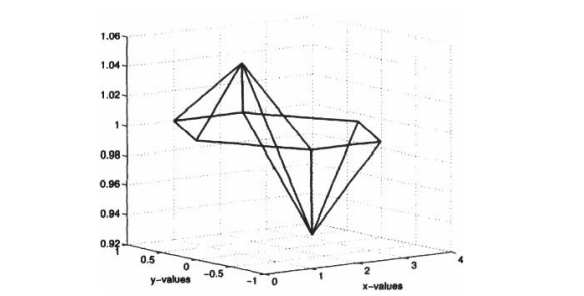
\includegraphics[width=1\linewidth]{17}
	\centering
	\label{pfig:ch13_17}
\end{figure}
\textbf{FIGURE 13.32:} Plot of our first FEM solution to the BVP of Example 13.5. Only 8 
elements and 2 internal nodes were used, so the plot is rather coarse. 
\\
\\
EXERCISE FOR THE READER 13.6: If in the BVP of Example $13.5$ we change the $B C$ to $u \equiv 2$ on $\partial \Omega$, but leave all else the same, how would the exact solution of this modified problem compare with that of the original? Perform the FEM on this modified problem (with the same triangulation) and compare the numerical solution with that of the original problem.
\\
\\
The resolution used in the last example was made deliberately coarse so that we could focus on the various facets of the FEM. We now move on to apply the FEM to a problem with a much more elaborate triangulation of the domain. The added complexity will force us to write some MATLAB loops to make the FEM feasible. The BVP we choose, the Laplace equation with Dirichlet boundary conditions on the unit disk, is rather special in that an explicit solution is available. We will thus be able to compare our FEM solution with the exact solution. Such examples are important as an aid for creating and testing production-level FEM codes. We state as a theorem this beautifully explicit result due to Poisson$^{11}$.
\begin{figure}[H]
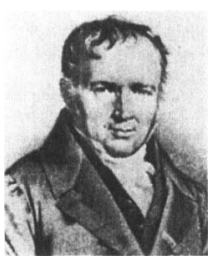
\includegraphics[width=0.35\linewidth]{18}
	\centering
	\label{pfig:ch13_17}
\end{figure}
\textbf{Figure 13.33:} Simeon-Denis Poisson (1781-1840), French 
mathematician.
\\
\\
\textbf{THEOREM 13.1:} (Poisson's Integral Formula) Suppose that $f(\theta)$ is a continuous function (given in polar coordinates) on the circle $x^{2}+y^{2}=R^{2}(\theta$ is the polar coordinate angle $)$. If $\Omega$ is the disk inside this circle, $\Omega=$ $\left\{p=(x, y) \in \mathbb{R}^{2}:\|p\|_{2}<R\right\}$, then the solution of the Dirichlet problem:
\begin{equation}
\left\{\begin{array}{lcl}
(\mathrm{PDE}) & \Delta u=0 & \text { on } \Omega \\
(\mathrm{BC}) & u(R, \theta)=g(\theta) & \text { on } \partial \Omega
\end{array}\right.
\end{equation}
is unique and is given by:
\begin{equation}
u(r, \theta)=\frac{R^{2}-r^{2}}{2 \pi} \int_{0}^{2 \pi} \frac{g(\phi) d \phi}{R^{2}-2 R r \cos (\theta-\phi)+r^{2}}
\end{equation}
Here, $(r, \theta)$ denotes the polar coordinates of any point inside $\Omega,(r<R)$.
\\
We omit the proof of this result (an enlightening one can be found in Section $4.6$ in the textbook [Ahl-79]). The result and proof actually extends to higher dimensions; see Section $7.5$ in [Zau-89] for the three-dimensional analogue. It turns out as well that the result remains valid for more general boundary data $f(\theta)$. For example, if $f(\theta)$ is only piecewise continuous, then $(20)$ will still solve the Dirichlet problem (19), and the solution will be continuous at all points on $\Omega \cup \partial \Omega=\left\{p=(x, y) \in \mathbb{R}^{2}:\|p\|_{2} \leq R\right\}$ except at those points on the boundary at which $f(\theta)$ is discontinuous (see again Section $4.6$ in the textbook [Ahl-79]). 
\footnotetext[11]{
 After his secondary education, Simeon-Denis Poisson went to work as a surgeon's apprentice with an 
uncle in Fontainbleau, a small city not far from Paris. His lack of coordination forced him to abandon 
his pursuit of this profession and he subsequently went to the local Ecole Central for undergraduate 
studies in search of a new career. His mathematical ability was noticed by his instructors who 
encouraged him to take the entrance exams at the premiere Ecole Polytechnique in Paris. Despite his 
relatively minor training, he placed at the very top and was admitted in 1798. His talents were quickly 
noticed and further cultivated by his teachers Laplace and Lagrange. Although his lack of manual 
dexterity precluded him from doing well in certain subjects (such as descriptive geometry), he excelled 
in subjects where drawing diagrams was not needed and at age 18 wrote a seminal memoir on finite 
differences which was well received. After graduation from Ecole Polytechnique he was offered a 
position there, a rare honor which he accepted. He spent the remainder of his career there and led a 
very productive life of contributions both to mathematics and physics. He cared deeply for 
mathematics and for maintaining the quality and sanctity of the Ecole Polytechnique. He was able to 
stop a group of politically active students at the Ecole from publishing a lampooning attack on 
Napoleon's leadership, fearing that this could do harm to the Ecole. He was elected to the physics 
section of the prestigious national Institute (a corresponding position in the mathematics section was not available; due to the limit set on membership a death of a member had to occur for a new slot to 
open). His name permeates many areas of mathematics and physics, which apart from differential 
equations ( Poisson bracket and integral formulas), include probability (Poisson distribution), harmonic 
analysis (Poisson summation formula), and elasticity (Poisson's ratio). During his career he wrote over 
300 research papers, but he was known never to work on more than one project at a time. He was 
extremely methodical and well-organized; if an idea for a new project would cross his mind while 
working on one paper he would write a brief note about it and place it in his wallet. After finishing one 
paper, he would then pull out all of the notes from his wallet to decide on the best topic for his next 
project.}
\\
This beautiful formula is one very rare instance where a general BVP has an explicit and practical solution. Recall that solutions of the Laplace PDE in (19) are called harmonic functions (Chapter 11). The BVP (19) can be viewed, for example, as finding the steady-state heat distribution of a circular plate whose temperature on the boundary is maintained with a certain known distribution $(f(\theta))$.
We will be able to use (20) to get MATLAB to run through a sufficiently fine set of nodes in the disk to obtain a plot of the exact solution. The nodes could be chosen to be those used in a FEM approximation so that the errors of the FEM solution could be examined. All of this will be done in Example 13.7$^{12}$
\\
\\
Example $13.5$ was intentionally set up so as to avoid the problem of having to numerically integrate functions of two variables. In more general examples, we will need to show how to deal with such integrals. MATLAB has an integrator to perform double integrals in floating point arithmetic. Such integrals can be time consuming depending on the oscillatory behavior of the integrand. Triangulations can be made finer in parts of the domain where the data functions have larger variations, and thus the integrals become less difficult to evaluate numerically. In practice, however, rather than using general integration programs or symbolic integrators, well-known quadrature approximations are employed. Such approximation schemes take advantage of the special structure of elements to approximate an integral over an element by a certain weighted average among certain special points of the element. We will present both approaches below. The first method will be to use MATLAB's numerical integrator. To facilitate general codes, we will appeal to some of the Symbolic Toolbox capabilities. The second method will utilize special quadrature formulas. The performance accuracy and times of both approaches will be compared and contrasted with an example where the exact solution can be obtained (and in which the FEM integrals will be quite simple). After presenting both methods, we will discuss some of the underlying theory. Particular readers may wish to cover only one method. Readers who do not have acceess to or wish to avoid using the Symbolic Toolbox may wish either to skip Method 1 , or to be prepared to recode those parts of it which appeal to symbolic functionality. In our numerical example (as we will see below), Method 2 ran about 200 times faster than Method 1 and gave the same quality of results. Such results are typical and this is why we recommend Method
2. We include Method 1 only for comparison purposes; for readers interested in practical codes, it may be skipped altogether.
\\
\\
\textbf{NUMERICAL APPROXIMATION TO DOUBLE INTEGRALSMETHOD 1: USING MATLAB's NUMERICAL INTEGRATOR \texttt{dblquad}:}
\\
\\
MATLAB's numerical integrator for double integrals has a syntax that requires the integration to be performed over a rectangle. We explain its functionality below and then show how it can be adapted to perform integrations over more general regions.
\begin{center}
\begin{tabular}{|c|l|}
\hline
&Assume that fun is an\\
& inline function of x and y$^{13}$\\
& This command will numerically\\& compute the integral \\
\texttt{dblquad(fun,xmin,xmax} &$\int_{x \min }^{x \operatorname{man}} \int_{\min }^{y \max } f u n(x, y) d y d x$\\ 
\texttt{ymin,ymax) ->}&using a double iteration with the single variable\\
& function integrator quad and with a default\\
& tolerance for error being le-6. As with \texttt{quad},\\
&the syntax of dblquad 
requires that we make the\\
& integrand \texttt{fun (x, y)} able to 
input a vector \\
&argument for (the first variable) x and return\\
& a vector of the same size.\\
\hline
&Optional extra inputs: \texttt{tol} allows specification of an error\\
\texttt{dblquad(fun,xmin,xmax}&tolerance, \texttt{@quadl} specifies that the more refined \texttt{quadl} \\
\texttt{ymin,ymax,}&integrator be used in the iterations, the last inputs \texttt{pi, p2},\\
\texttt{tol,@quadl,pi,p2,... )}& ... represent numerical values to assign in case \texttt{fun}\\
\texttt{->}&depends on additional parameters:"\texttt{fun =} \\
&\texttt{fun(x,y,pl,p2,...).}\\
\hline
\end{tabular}
\end{center}
\footnotetext[12]{As an aside, we point out here some related facts. A celebrated result in the theory of complex variables (which can be found in [Ahl-79], the classic treatise on the subject) known as the Riemann mapping theorem, states that any simply connected planar domain $D \subset \mathbf{R}^{2}$ can be mapped conformally onto the unit disk $U=\left\{p=(x, y) \in \mathbf{R}^{2}:\|p\|_{2}<1\right\}$. Simply connected means roughly that the domain has no holes inside, i.e., if $\gamma$ is any closed path in the domain, then the interior of $\gamma$ contains only points in the domain; see [Ahl-79] for more details. A conformal mapping is a one-to-one function (of two variables) $F$ such that $F(D)=U$. Conformal mappings have the property that they preserve angles and have many beautiful properties (see [Ahl-79]). One particularly useful property of conformal mappings is that they preserve harmonic mappings, i.e., if $u(x, y)$ is a harmonic function on the domain $U$ and $F: D \rightarrow U$ is a conformal mapping, then $v=u(F(x, y))$ is a harmonic function on $D$. This result means that for any simply connected domain in the plane, there is a corresponding Poisson integral formula for solutions of the Dirichlet problem gotten by changing variables to the disk. This is quite a satisfying and complete result, theoretically, at least. The practical problem for a given simply connected domain thus reduces to computing explicity a function which conformally maps it to the disk $U$. This problem has been extensively studied and there are many situations where the mappings have been found. This approach has led to numerous applications to physical BVPs involving the Laplace equation, including also steady-state fluid flow, and electrostatics. See [BrChSi-03] for more on conformal mapping with an emphasis on applications.}
The following simple example will illustrate the syntax requirement on \texttt{fun}
\\
To evaluate the integral of $x^{2} y^{2}$ over the rectangle $R=[0,2] \times[1,2]$ :
$$
\int_{R} x^{2} y^{2} d x d y=\int_{0}^{2} \int_{1}^{2} x^{2} y^{2} d y d x,
$$
we could simply enter:
\\
\\
\texttt{$>>\text { dblquad(inline }('x.^{\wedge}2.^{*}y.^{\wedge}{2}, ' x^{\prime}, ' y^{\prime}), 0,2,1,2) \quad \rightarrow \text { ans }=6.2222$}
\\
\\
The vector syntax requirement on the first variable $x$ is automatically satisfied since this variable appears in the single term for the integrand. If, however, we wanted (for testing purposes) to compute the area of the rectangle $R$, the corresponding command:
\\
\\
\texttt{$>>\text { dblquad (inline }(' 1 ', x^{\prime}, ' y^{\prime}), 0,2,1,2)$}
\\
\footnotetext[13]{As usual, if instead "fun" has been stored as an M-file, it should be written with single quotes: dblquad ('fun",..) or preceded with the "@" symbol: dblquad (@fun, ...).}
\\
gives a series of error messages:
\\
??? Index exceeds matrix dimensions.
\\
\\
\texttt{$Error~ in~ $==>$ C:\backslash MATLAB6p5\backslash toolbox\backslash matlab\backslash funfun\backslash quad.m$}
\texttt{On line 67 $==>$ if \textasciitilde isfinite(y(7))}
\\
(more...)
\\
\\
The syntax can be adjusted accordingly as follows:
\\
\texttt{$>>\text { dblquad (inline }(' 1^{*}ones(size(x))'x^{\prime}, ' y^{\prime}), 0,2,1,2)$
\\
\texttt{->ans=2}
}
\\
\\
which (as we know) gives the correct answer. A similar syntax note was pointed out in Chapter 3 for quad.
\\
\\
In order to use dblquad to integrate over regions other than rectangles the following identity will be useful:
\\
\begin{equation}
\begin{aligned}
&\int_{T} \text { fun }(x, y) d x d y \equiv \int_{\mathrm{xmin}}^{\mathrm{xmax}} \int_{\operatorname{ylow}(x)}^{\operatorname{ytop}(x)} \text { fun }(x, y) d y d x \\
&\quad=\int_{\mathrm{xmin}}^{\mathrm{xmax}} \int_{0}^{1} \text { fun }(x, \operatorname{ylow}(x)+u(y \operatorname{top}(x)-\operatorname{ylow}(x)))[y \operatorname{top}(x)-\operatorname{ylow}(x)] d u d x,
\end{aligned}
\end{equation}
\begin{figure}[H]
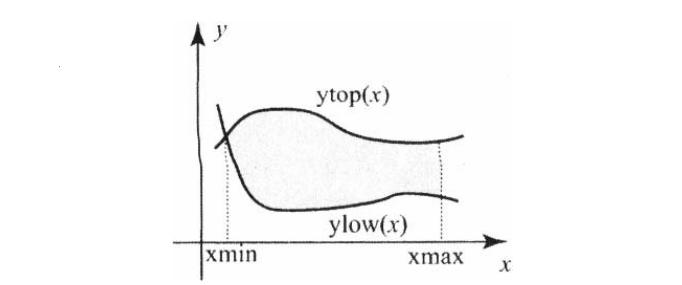
\includegraphics[width=0.9\linewidth]{20}
	\centering
	\label{pfig:ch13_17}
\end{figure}
\textbf{FIGURE 13.34:} Illustration of a typical planar region on which integrals can be computed 
using (21). 
\\
\\
Here, the region $T$ need not be a triangle, but rather any region in the plane bounded below by the curve ylow $(x)$ and above by the curve ytop $(x)$ and over the range [xmin, xmax]; see Figure 13.34.
\\
\\
The identity (21) is easily established by a simple variable substitution; see Exercise 20. Using this identity, we may use dblquad to compute any double integral. Since all of our integrals in the text proper of this section will be over triangles, the next example will present some more or less typical evaluations of double integrals over triangles.
\\
\\
EXAMPLE 13.6: Let the triangle $T$ of Figure $13.30$ have the following vertices: $v_{1}=(1,3), v_{2}=(5,1)$, and $v_{3}=(4,6)$. Use MATLAB's dblquad to numerically compute the following integrals:
\\
\\
(a) $\int_{T} 2 x y^{2} d x d y$
\\
\\
(b) $\int_{T} \sin (x y \sqrt{y}) d x d y$
\\
\\
In each, decrease the tolerance or change to quadl, as needed, until the answers agree to four decimals.
\\
\\
SOLUTION: We need first to express the integrals as double integrals. Letting $x$ be the outer integration variable, the $x$-range of $T$ is $1 \leq x \leq 5$. Over this range, the lower function ylow of $x$ will be the line segment from $v_{1}$ to $v_{2}$ (see Figure 13.30). Writing this line segment as a function of $x$ yields: ylow $(x)=-\frac{1}{2} x+\frac{7}{2}$. The corresponding upper function ytop of $x$ splits up into two formulas determined by the two segments $v_{1} v_{3}$ and $v_{3} v_{2}$. Writing each of these segments as a function of $x$ yields the following formula for $y$ top: $\operatorname{ytop}(x)= \begin{cases}x+2, & \text { if } x \leq 4 \\ -5 x+26, & \text { if } x>4\end{cases}$
\\
\\
\\
Part (a): Using the above functions, we can rewrite the integral in the following 
iterated form: 
$$
\int_{T} 2 x y^{2} d x d y=\int_{1}^{5} \int_{\text {ylow }(x)}^{\text {ytop }(x)} 2 x y^{2} d y d x=\int_{1}^{4} \int_{\text {ylow }(x)}^{x+2} 2 x y^{2} d y d x+\int_{4}^{5} \int_{\text {ylow }(x)}^{26-5 x} 2 x y^{2} d y d x
$$
\\
The latter form is a more convenient one to implement on MATLAB. The code 
given below is written in a way that will make it easy to adapt to handle the 
general computation of such integrals and to this end it is more convenient to use 
some Symbolic Toolbox capabilities. 
\\
\texttt{$>>$ syms $x y u$\\
$>>$ ylow $=-.5 * x+3.5 ;$ ytop $1=x+2 ; \quad$ ytop $2=-5 * x+26 ;$\\
$>>$ f $u n=2 * x^{\star} y^{\wedge} 2$;\\
$>>$ ynew $1=y$ low $+u^{*}(y$ topl $-y$ low) ;\\
$>>$ funprepl =subs (fun, $Y$, ynew 1$) *(y$ top $1-y l o w)$;\\
$>>$ ynew $2=y l o w+u^{*}(y$ top2 $-y$ low) ;\\
$>>$ funprep2=subs (fun, y, ynew 2$) *(y$ top $2-y$ low $)$;\\
$>>$ funnew $1=$ vectorize (inline $\left(\left[\operatorname{char}(\right.\right.$ funprepl $)$, ones $\left.^{\prime}(\operatorname{size}(u))^{\prime}\right], \ldots$
$$
\left.\left.' u^{\prime}, x^{\prime}\right)\right) \text {; }
$$
$>>$ $\%$we needed to convert the symbolic expression back into a\\
$>>$ $\%$character string for construction of an inline function.\\
$>>$ funnew $Z=$ vectorize (inline ( [char (funprep 2$), ' *$ ones $($ size (u) $) '], \ldots$
$' u ',(x+))$;\\
$>>$dblquad (funnew $1,0,1,1,4)+$ dblquad (funnew $2,0,1,4,5$ )\\
\\
$\rightarrow ans = 724.8000$ }
\\
\\
\text { Using a smaller tolerance (than the default } $10^{-6}$ \text { ) gives the same result: }
\\
\texttt{$>>$ dblquad ( funnew $1,0,1,1,4,1 e-7)+\mathrm{dblquad}$ (funnew2, $0,1,4,5,1 e-7$)
\\
$
\rightarrow \text { ans }=724.8000
$}
\\
\\
Part (b) Implementing the same strategy, we obtain: 
\\
\\
\texttt{$>>f u n=\sin \left(\sin (x)^{\star} y\right) ;$\\
$>>$ funprepl $=$ subs (fun, y,ynewl) * (ytopl-ylow) ;\\
$>>$ funprep2=subs $(f u n, y$, ynew 2$) *(y \operatorname{top} 2-y l o w) ;$\\
$>>$\\
funnew1 = vectorize$\left(\right.$ inline ( $\left[\operatorname{char}\right.$ (funprepl),' ${ }^{\prime}$ ones $\left.\left.\left.(\operatorname{size}(\mathrm{u}))^{\prime}\right], \mathrm{u}^{\prime}, \mathrm{x}^{\prime}\right)\right)$\\
$>>$\\
funnew2 =vectorize (inline ( $\left[\operatorname{char}(\right.$ funprep 2$),{ }^{\prime}{ }^{*}$ ones $\left.\left.\left.(\operatorname{size}(\mathrm{u}))^{\prime}\right], \mathrm{u}^{\prime}, \mathrm{x}^{\prime}\right)\right)$\\\
$>>$ dblquad (funnew $1,0,1,1,4)+$ dblquad (funnew $2,0,1,4,5)$
$\rightarrow$
\\ ans $\rightarrow 0.1397$}
\\
\\
There is agreement when we reduce the tolerance as above. 
\\
\\
The numerical integration(s) of part (b), unlike that in part (a), took a noticeable amount of time. This is due to the fact that the integrand in part (b) is very oscillatory over the domain. In general, double integrals can take a lot of work to evaluate effectively since, if the integrals cannot be done explicitly, any method basically has to iterate evaluations of a one-variable integral on numerous slices (the number goes up when more accuracy is desired). When performing the FEM to solve a given BVP, the triangulation can and should be done so as to use smaller elements in areas of high oscillation of the given data. This will assure that the integrals that arise in the assembly process will be numerically quite tame and easy to compute. MATLAB's symbolic integrator \texttt{int} can also be used to evaluate double integrals, and although the syntax is a bit simpler than for \texttt{dblquad}, the M-files we introduce below will help to make \texttt{dblquad} more convenient to use. Also, the extra computing time needed for \texttt{int} to attempt to find exact antiderivatives, which is usually not possible in general, is not worth the occasional extra precision in the answers.
\\

To save on having to go through the above complicated syntax each time a numerical integral is encountered, we give here an M-file that is essentially a userfriendly version of \texttt{dblquad}. It is a simple modification of the code employed in the last example.
\\
\\
\textbf{PROGRAM 13.1:} User-friendly M-file for numerically computing double integrals over planar regions bounded between two functions of $x$, as in Figure 13.34. Integrand fun is entered as a function of the symbolic variables $x$ and $y$.
\\
\\
\\

\texttt{function nint= quad2d(fun,xmin,xmax,ylow, ytop)} \\
\texttt{$\%$ numerically computes a double integral of a function 'fun on a'}\\
\texttt{$\%$region over the interval $minx<x<maxx$ and between the functions of}\\
\texttt{$\%$x: $ylow<y<ytop$.}\\
\texttt{$\%$ INPUTS: fun = a function of the symbolic variables x and y}\\
\texttt{$\%$ minx = minimum x-value for regin}\\
\texttt{$\%$ maxx = maximum x-value for region}\\
\texttt{$\%$ ylow = function of symbolic variables for lower boundary of region}\\
\texttt{$\%$ ytop = function of symbolic variables for lower boundary of region}\\
\texttt{$\%$ OUTPUT: nint = numerical approximation of integral using the}\\
\texttt{$\%$ integrator 'dblquad' in conjunction with the default settings.}\\
\texttt{$\%$ x and y should be declared symbolic variables before this M-file is}\\
\texttt{$\%$ used.}\\
\texttt{syms $u x y$
ynew$=ylow+u^{*}$ (ytop-ylow);\\
funprep=subs(fun, $y$, ynew) $\*$ (ytop-ylow);\\
funnew=vectorize (inline ([char (funprep),$ *($;}\\
\\
EXERCISE FOR THE READER 13.7: Use the above program to numerically compute the following double integrals:
\\
\\
(a) $\int_{S} x y^{2} d x d y$, where $S$ is the circular sector $\{(r, \theta): 0 \leq r \leq 1,0 \leq \theta \leq \pi / 4\}$.
\\
\\
(b) $\int_{U} \exp \left(1-x^{2}-2 y^{2}\right) d x d y$, where $U$ is the region enclosed between the curves $y=e^{x}, y=x^{2}-1$ and $y=0$.
\\
\\
EXERCISE FOR THE READER 13.8: (a) Write an M-file, \texttt{integ= triangquad2d (fun,v1,v1,v3}) whose inputs are a function of $\mathbf{x}, \mathbf{y}$ (written as a symbolic expression), and three $2 \times 1$ matrices \texttt{$v 1, v 2, v 3$} which are vertices (in any order) of triangle in the $x y$-plane. If we denote this triangle by $T$, the output \texttt{integ} will be the numerical integral $\int_{T}$ fun $(x, y) d x d y$, computed with \texttt{quad2d} as in Example 13.6.
\\
\\
(b) Use your function in Part (a) to reevaluate the integrals of Example 13.6, and also to compute the following integrals in which $T_{1}$ is the triangle with vertices $(0,0),(6,0),(12,2)$, and $T_{2}$ is the triangle with vertices $(1,3),(3,2)$, and $(2,5)$.
\\
(i) $\int_{T_{1}} 1 d x d y=6$,\\
(ii) $\int_{T_{2}} 1 d x d y=5 / 2$,\\
(iii) $\int_{T_{1}} 2 x^{2} d x d y=504$, and\\
(iv) $\int_{T_{2}} \sin \left(x^{2}\right) d x d y \approx-0.2998$
\\
\\
\textbf{Suggestions:} Branch your program off into two cases: Either the triangle has a vertical side or the three $x$-coordinates of the vertices are distinct. Draw lots of pictures of triangles as you are proceeding.
\\
\\
\textbf{EXAMPLE 13.7:} Consider the Dirichlet problem (19) on the unit disk $\Omega=\left\{(x, y): x^{2}+y^{2}<1\right\}$
\\
$$
\left\{\begin{array}{lrlrl}
(\mathrm{PDE}) & \Delta u & =0 & & \text { on } \Omega \\
(\mathrm{BC}) & u(1, \theta) & =g(\theta) & & \text { on } \partial \Omega
\end{array}\right. \text {, }
$$
(we put $R=1$ in (19)), where $g(\theta)=\left\{\begin{array}{ll}2 \theta^{2}, & \text { if } 0 \leq \theta \leq 2 \\ 8, & \text { if } 2<\theta \leq 3 \\ 0, & \text { if } 3<\theta \leq 2 \pi\end{array}\right.$.
\\
\\
(a) Use the FEM with a triangulation of the disk involving between 50 and 100 nodes deployed on circles of increasing radii but more or less uniformly (as in Method 2 of the solution to Example 13.2(a) of the last section) to solve this BVP and plot the FEM solution.
(b) Use the Poisson integral formula (20) to numerically compute the exact solution at each of the nodes in part (a), and plot it. Compare with the plot obtained in part (a), and compute the maximum error (at the interior nodes).
(c) Repeat both parts (a) and (b), this time using between 500 and 1000 nodes.
\\
\\
\textbf{SOLUTION:} Part (a): The triangulation can be done in exactly the same fashion as was done in Method 2 of part (a) of the solution of Example $13.2$ (simply change the value of delta=sqrt (pi/90); everything else is the same). The code is thus omitted here; the nodes were stored in vectors $x$ and $y$ and the triangulation in the matrix tri. The triangulation is shown in Figure 13.35.
\begin{figure}[H]
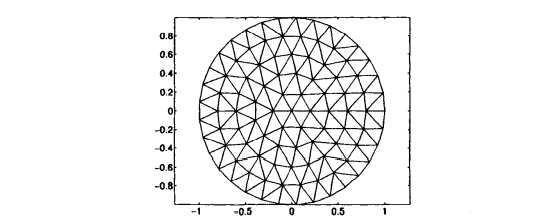
\includegraphics[width=0.9\linewidth]{21}
	\centering
	\label{pfig:ch13_21}
\end{figure}
\textbf{FIGURE 13.35:} Triangulation for the FEM solution of Example 13.7(a). There are 99 
nodes and 163 triangular elements.
\\
\\
By the way in which the nodes were created, the numbering scheme conforms to that of the procedure outline (the boundary nodes are indexed last). In the notation of the procedure, $m=99$ (= total number of nodes), as seen by entering \texttt{size(x).} We can use a simple MATLAB loop to compute $n$ (= number of interior nodes):
\\
\\
\texttt{$>>$ n=l;\\
$>>$ while $x(n)^{\wedge} 2+y(n)^{\wedge}2<1-eps$
\\      n=n+l;
\\ end
\\ $>>$ n=n-l -> n = 66 }
\\
\\
(Note: We used \texttt{eps} (= machine epsilon) to safeguard the inequality from 
roundoff errors.) Thus there are n = 66 interior nodes.
\\
\\
We now use the boundary data to assign the corresponding coefficients $c_{i}(i>n)$
\\
\\
of the basis functions for thefor the FEM solution $v=\sum^{m} c_{i} \Phi_{i^{*}}$ To facilitate this, we will create an M-file for the boundary data function $g(\theta)$. Since the function will eventually need to be integrated (in part (b) when we use the Poisson integral formula), and the function is defined by cases, we will implement the special vector construction for this $M$-file that was explained in Chapter 4 :
\\
\\
\texttt{function y = EX13$\_$7$\_$ bdydata(x)}\\
\texttt{for i = 1:length(x)}\\
\texttt{if $(0<=x(i))\&(x(i)<=2)$}

~~\texttt{$y(i)=2*x(i)^{\wedge}2 ;$}\\
\texttt{elseif $(2<x(i))$\&$(x(i)<=3)$}

~~\texttt{$y(i)=8$;}\\
\texttt{else}

~~\texttt{$y(i)=0$;}\\
\texttt{end}\\
\texttt{end}
\\
\\
Now, since the boundary data function is a function of the angle $\theta$, and the nodes are stored as ordered pairs of $x y$-coordinates, in order to use this function to assign the node coefficients, we must compute and input the corresponding angles for each node. MATLAB has the following built-in functions for such coordinate changes:
\\
\\
\begin{center}
\begin{tabular}{|c|l|}
\hline
&If (x, y) denote the cartesian coordinates of a point in the\\
&plane, the output [\texttt{th, r}] will be the corresponding polar\\
\texttt{[th,r]=cart2pol (x,y) ->}&coordinates, where the angle th is chosen in the interval 
\\&($-\pi ,\pi$], and the radius r is nonnegative.\\
\hline
\texttt{[x,y]=pol2cart(r,th) ->} &Inputs a set of polar coordinates (\texttt{r,th}) and outputs the\\
&orresponding cartesian coordinates.\\
\hline
\end{tabular}
\end{center}
The following loop will now store the boundary node coefficients:
\\
\\
\texttt{for i=67:99}

~\texttt{th=cart2pol(x(i),y(i)); 
}

~\texttt{if th<0, th=th+2*$\pi$ ; end}

~\texttt{\% need to ensure th is in domain of boundary data function}

~\texttt{c(i)=EX13\_ 7\_ bdydata(th);}
\texttt{end}
\\
\\
We are now ready to move on to the assembly process. We first observe that since (in the notation of $(10)), q \equiv 0, f \equiv 0$ and $p \equiv 1$, equations $\left(15^{\prime}\right)$ and $(16^{\prime})$ simplify to:
$$
a_{\alpha \beta}^{l}=\int_{T_{1}}\int \nabla \Phi_{i_{a}} \cdot \nabla \Phi_{i_{\beta}} d x d y(1 \leq \alpha, \beta \leq 3)
$$
and
$$
b_{\alpha}^{l}=-\sum_{s=n+1}^{m} c_{s} \int_{T_{l}}\int \nabla \Phi_{s} \cdot \nabla \Phi_{i_{a}} d x d y \quad(1 \leq \alpha \leq 3)
$$
respectively. Also, of the 33 possible indices $s$ in the $b_{\alpha}^{l}$ formulas, only those (at most two) corresponding to boundary nodes of the element $T_{l}$ need to be considered. Since each gradient appearing in the above integrals is of a linear function on an element, the integrands are all constants, and so the corresponding integrals will be simply the constant times the area of the underlying element. We will use the M-file of Exercise for the Reader $13.8$ to evaluate each of these integrals (within a loop).
\\
\\
We will make use of MATLAB's \texttt{setdiff} built-in function, which was introduced in the last section, but with an optional second output variable.
\begin{center}
\begin{tabular}{|c|l|}
\hline
&The first output variable was explained in the last\\
\texttt{[d,ind] = setdiff(a,b ) ->}&section. The optional second output variable will be the\\
&indices of a which produce the vector d.\\
\hline
\end{tabular}
\end{center}
Here is a brief usage example: 
\\
\\
\texttt{>> a = [1 2 3] ; b = [2 4] ;}\\
\texttt{>> d * setdiff (a,b) -> d=1 3}\\
\texttt{>> a = [3 2 1] ;}\\
\texttt{>> [d,ind] = setdiff(a, b) ->d=1 3, ind=3 1}\\
\\
As usual, we first initialize the $n \times n(n=66)$ stiffness matrix $A$ of zeros and the corresponding $n \times 1$ initial load vector $b$ and create a program that will completely perform the assembly. Here is the complete code for the assembly process for Example 13.7.
\\
\\
\texttt{>> N=[x' y'];}\\
\texttt{>> E=tri;}\\
\texttt{>> n=66; m=99; syms x y}\\
\texttt{>> A=zeros(n); b=zeros(n,1);}\\
\texttt{>> [L cL]=size(E);}\\
\texttt{>> for ell=l:L}

~\texttt{nodes=E(ell,:); }

~\texttt{intnodes=nodes(find(nodes<=n)); }

~\texttt{bdynodes=nodes(find(nodes>n)) ;}

~\texttt{\% find gradients [a b] of local basis functions}

~\texttt{\% ax + by + c; distinguish between int node}

~\texttt{\% local basis functions and bdy node local basis}

~\texttt{\% functions}\\
\\
\texttt{for i=l-.length (intnodes)}

~\texttt{xyt=N(intnodes(i),:); \% main node for local basis function}

~\texttt{onodes=setdiff(nodes,intnodes(i) );}

~\texttt{\% two other nodes (w/ zero values) for local basis function}

~\texttt{xyr=N(onodes(1),:); 
}

~\texttt{xys=N(onodes(2),:);}

~\texttt{M= [xyr 1; xys 1; xyt 1 ] ; \% matrix M of (4) }

~\texttt{abccoeff=[xyr(2)-xys(2); xys(1)-xyr(1); xyr(1)*xys(2)-... 
}

~\texttt{xys(1)*xyr(2)]/det(M); \% coefficents of basis function on triangle \# L }

~\texttt{\% See formula (6a)}

~\texttt{intgrad(i,:)=abccoeff(1:2)';}
\\
\texttt{end}
\\
\\
\texttt{for j=l:length(bdynodes)}

~\texttt{xyt=N(bdynodes (j) , :) ; \% main node for local basis function}

~\texttt{onodes=setdiff (nodes,bdynodes (j)) ; '\% two other nodes}

~\texttt{\% (w/ zero values) for local basis function}

~\texttt{xyr=N(onodes(1),:);}

~\texttt{xys=N(onodes(2),:); 
}

~\texttt{M=[xyr l;xys l;xyt 1]; \% matrix M of (4) }

~\texttt{abccoeff=[xyr(2)-xys(2); xys(1)-xyr(1); xyr(1)*xys(2)-... 
}

~\texttt{xys(1)*xyr(2)]/det(M); \% coefficents of basis function on triangle \# L }

~\texttt{bdygrad(j,:)=abccoeff(1:2) ; 
}
\\
\texttt{end}
\\
\\
\texttt{\% update stiffness matrix}\\
\texttt{for il=l:length(intnodes)}\\
\texttt{for i2=l:length(intnodes)}

~\texttt{fun = sym(intgrad(il,:)*intgrad(i2, :)') ; \% integrand for (15ell)}

~\texttt{integ=triangquad2d(fun,xyt,xyr,xys);}

~\texttt{A(intnodes(il),intnodes(i2))=A(intnodes(il),intnodes(i2))+integ; }
\texttt{end}\\
\texttt{end}
\\
\\
\texttt{\% update load vector}\\
\texttt{for i=l:length(intnodes) }\\
\texttt{for j=l:length(bdynodes)}

~\texttt{fun = sym(intgrad (i, :) *bdygrad (j,:)') ; \% integrand for part of (16ell)}

~\texttt{integ=triangquad2d(fun,xyt,xyr,xys);}

~\texttt{(intnodes(i))=b(intnodes(i))-c(bdynodes(j))*integ; }

~\texttt{end}

~\texttt{end}\\
\texttt{end}\\
\texttt{sol=A/b }\\
\texttt{c(l:n)=sol';}\\
\\
The result is now easily plotted using the \texttt{trimesh} function of the last section: 
\\
\\
\texttt{>> x=N(:,l) ; y=N(:,2) ;}\\
\texttt{>> trimesh(E,x,y,c), xlabel('x-values'), ylabel('y-values') 
}\\
\texttt{>> hidden off 
}\\
\\
The resulting plot is shown in Figure 13.36.
\begin{figure}[H]
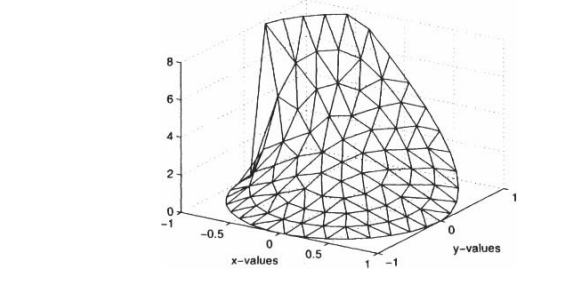
\includegraphics[width=0.9\linewidth]{22}
	\centering
	\label{pfig:ch13_22}
\end{figure}
\textbf{FIGURE 13.36}: Plot of the FEM solution of the Dirichlet problem of Example 13.7.
Part (b): The following simple loop will implement the Poisson integral formula (20) to determine the value of the exact solution at each of the interior nodes $c_{i}(i \leq n)$. As has been the convention thus far, we continue to use MATLAB's numerical integrators for one-dimensional integrals; in this case we use quadl. We will leave the already assigned values at the boundary nodes $c_{i}(i>n)$. We first create and store an M-file for the integrand in the Poisson integral formula (20) using the boundary data of the current example. Since this function will be integrated (with quadl) we will need to construct it as shown in Chapter 4 so that it will appropriately handle vector inputs.
\\
\\
\texttt{function y = EX13\_7\_poisson(phi,r,th) }\\
\texttt{for i = 1:length(phi)}\\
\texttt{if (0<=phi(i))\&(phi(i)<=2)}

~\texttt{y(i)=2*phi(i) 2*(1-r 2)/2/pi/(l-2*r*cos(th-phi(i))+r 2); 
}\\
\texttt{elseif (2< phi(i))\&( phi(i)<=3) }

~\texttt{y(i)=2*phi(i) 2*(1-r 2)/2/pi/(l-2*r*cos(th-phi(i))+r 2); 
}\\
\texttt{else}

~\texttt{y(i)=0;}\\
\texttt{end}\\
\texttt{end}
\\
\\
\texttt{>> cp=c; \%initialize node values for Poisson integral method. }\\
\texttt{>> for i=l:n}\\
\texttt{[th, r]=cart2pol(N(i,1),N(i,2)); \%polar coors for node \#i}\\
\texttt{cp(i)= quadl(@EX13\_7\_poisson, 0,3,[],[],r,th);}\\
\texttt{\%since integrand vanishes on (3, 2*pi] we can reduce the interval of}\\
\texttt{\%intgration.}\\
\texttt{end}
\\
\\
The plot of the exact solution just obtained ${ }^{14}$\footnotetext[14]{Of course, the Poisson integral formula, as mentioned, is exact. The only errors will be the errors that arise from the numerical integration. By default, the accuracy goal will have error $<1 e-6$, and the integrand is well-behaved so such errors will not be relevant for our present comparison purposes. In case they do become relevant (with a much finer mesh, say), we could always set a new accuracy goal for quadl.}
 will be quite similar to that of our FEM approximation in Figure 13.36. The resulting error plot is now easily obtained by the following commands, and the plot is shown in Figure 13.37.
\\
\\
\texttt{>> trimesh(E,x,y,abs(c-cp))}\\
\texttt{>> hidden off }\\
\texttt{>> xlabel('x-values'), ylabel('y-values') }
\\
\\
Part (c): The code in parts (a) and (b) is written in a way so that just one small change in one line of the code is required to do part (c). In the creation of the nodes (as in Method 2 of in the solution of Example 13.2(a)) we only need to change the paratmer $\delta$ to $\sqrt{\pi / 900}$. The resulting node set contains $m=897$ nodes of which the first $n=791$ are interior nodes, and the Delaunay triangulation contains 1686 elements. The main loop took close to an hour on the author's computer. See Figure $13.38$ for plots of the FEM solution and error.
\begin{figure}[H]
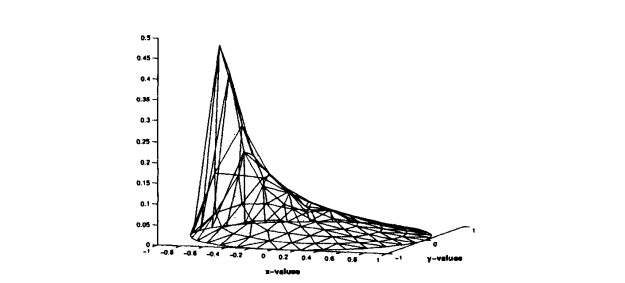
\includegraphics[width=0.9\linewidth]{23}
	\centering
	\label{pfig:ch13_23}
\end{figure}
\textbf{FIGURE 13.37}: Plot of the error of the FEM solution of Example 13.7, obtained by 
comparing it to the exact solution over the same grid from the Poisson integral formula$^{15}$ \footnotetext[15]{More preciselely, this plot is the difference between the FEM solution and the piecewise linear 
interpolant of the exact solution. }
\\
\\
(and triangulation) and computes the corresponding FEM solution of a BVP. For each element, the $z$-stretch (the difference of maximum and minimum $z$-values of FEM solution over just the element) is recorded and those for which this stretch is in, say the largest $10 \%$ or exceeds a certain numerical value (this can be adjusted) are flagged. In the vicinity of such elements, extra nodes are added and a new mesh is created. This is iterated a certain number of times (which can be adjusted) or until the maximum $z$-streches fall below a certain prescribed value (which also can be adjusted). Such an adaptive scheme will be addressed in the exercises of this section.
\\
\\
EXERCISE FOR THE READER 13.9: Use the FEM with a triangulation of the disk involving roughly 100 nodes deployed in a way so that more nodes are used near $(x, y)=(\cos (3), \sin (3))$ to solve the BVP Example 13.7. Can you triangulate in such a way that the maximum error is smaller than that obtained in the solution of part (b) of Example $13.7$ (when 897 nodes were used)? Plot the error (as computed above using the Poisson integral formula).\\
\textbf{Suggestion:} Try several different schemes with the main goal being to minimize the maximum total error (i.e., the $z$-height of the error graph). The node sets are small enough so that CPU time will not hinder multiple experiments.\\
\\
\textbf{NUMERICAL APPROXIMATION TO DOUBLE INTEGRALS-
METHOD 2: APPROXIMATION QUADRATURE FORMULAS 
(RECOMMENDED): }
\\
Suppose that $T$ is a region in the plane. A so-called Gauss quadrature formula for approximation of general integrals over $T$ takes the form:
\begin{equation}
\int_{T} f(x, y) d x d y \approx w_{1} f\left(\xi_{1}\right)+w_{2} f\left(\xi_{2}\right)+\cdots+w_{n} f\left(\xi_{n}\right)
\end{equation}
where the \textbf{weights} $w_{1}, w_{2}, \cdots, w_{n}$ are specified real numbers and the \textbf{sampling points} $\xi_{1}=\left(x_{1}, y_{1}\right), \quad \xi_{2}=\left(x_{2}, y_{2}\right), \quad \xi_{1}=\left(x_{1}, y_{1}\right), \xi_{2}=\left(x_{2}, y_{2}\right), \cdots, \xi_{n}=\left(x_{n}, y_{n}\right)$ are specified points in $T$. In general, these formulas are developed with the goal that they be exact for polynomials (in two variables) up to a specified degree. If such a formula was exact for polynomials of degree up to $p$, Taylor's theorem in two variables could then be used to show that if the integrand has continuous partial derivatives up to order $p+1$ then the crror of the approximation (22) is $O\left(h^{p+1}\right)$, where $h$ is the diameter of $T$ (Exercise 28). For each sampling point there are three degrees of freedom (the weight, and the coordinates of the sampling point). For example, when $T$ is a triangle with vertices $V_{1}, V_{2}$, and $V_{3}$ it can be shown (Exercise 29) that the following formula is exact for any polynomial of degree at most one:
\begin{equation}
\int_{T} f(x, y) d x d y \approx \frac{\operatorname{Area}(T)}{3}\left\{f\left(V_{1}\right)+f\left(V_{2}\right)+f\left(V_{3}\right)\right\}
\end{equation}
This may be interpreted as a two-dimensional generalization of the trapezoidal rule. With the same number of sample points we can do better: If we choose them to be the midpoints of the edges of the triangle, rather than the vertices, we arrive at the following formula that turns out to be exact for polynomials of degree at most 2:
\begin{equation}
\int_{T} f(x, y) d x d y \approx \frac{\operatorname{Area}(T)}{3}\left\{f\left(\left[V_{1}+V_{2}\right] / 2\right)+f\left(\left[V_{1}+V_{3}\right] / 2\right)+f\left(\left[V_{2}+V_{3}\right] / 2\right)\right\}
\end{equation}
For a brief but enlightening introduction on how such formulas are derived, see Section $5.2$ of [ZiMo-83]. More details can be found in the article [Cow-73]; see also [Kry-62].
\\
\\
EXERCISE FOR THE READER 13.10: (a) Write an M-file for the Gaussian quadrature formula (24) having the following syntax:
$$
\texttt{int = gaussianintapprox(f, VI, V2, V3) 
}
$$
The input variables are: $f$, an inline function or an M-file, and $V 1, V 2$, and $V 3$, the vertices of a triangle in the plane (listed as row vectors of length two). The output \texttt{int} is a number corresponding to the integral approximation of (24).
(b) Run through the MATLAB codes of part (c) of Example $13.7$ on your own computer, and take note of the time it takes for the main finite element part of the code (after the triangulation). Then rewrite this part of the code to use the M-file of part (a) of this exercise in place of \texttt{dblquad}, and compare the resulting error and runtime.
\\
\\
Example $13.7$ gives a nice demonstration of how refinements of the mesh will reduce the errors of the FEM approximations of the actual solution. In general, if the data for the BVP (10) satisfy: $p, q$, and $f$ are piecewise continuous on $\Omega$, the first partial derivatives of $p q$, and $g$ are piecewise continuous on $\Gamma_{1}, r$ and $h$ are piecewise continuous on $\Gamma_{2}$ and $p(x, y) \geq p_{0}>0, q(x, y) \geq 0$, then it can be shown that with the above FEM scheme (as well as the one below for more general boundary conditions), the error of the FEM approximation is of order $\delta$, where $\delta$ is the maximum diameter of any of the (triangular) elements. This result can be roughly expressed by the following inequality:
\begin{equation}
\|u-\hat{u}\| \leq C \delta
\end{equation}
Here $u$ represents the exact solution of the BVP, $\hat{u}$ is the FEM solution (corresponding to a triangular mesh with $h$ defined as above), and $C$ is a constant that depends on the problem but not on $\delta$. The norm on the left can be any of several norms to measure the errors. The order of the errors can be upgraded from $\delta$ to higher powers of $\delta$ by using basis functions that are locally polynomial of higher degree (some examples of such elements were given in the exercises of the previous section). To give more specific results would require a deeper theoretical discussion involving some functional analysis. We refer the interested reader to Chapter 4 of [Joh-87]; see also [Cia-02] and [StFi-73]. We caution the reader that the situation of the Dirichlet problem on a disk for the Laplace PDE is very atypical in that an explicit solution is available (Theorem 13.1). The next two exercises for the reader will involve slight variations of this PDE; the first one deals with the same type of BVP but on another domain, while the second deals with a slightly different PDE (Poisson's) on the disk. It may come as a surprise that for such mild variations, no explicit solution techniques are known.
\\

From our experience with both methods of numerical quadrature applied to the same problem of Example 13.7, we see that in any FEM program, the amount of time devoted to numerical quadrature is a crucial consideration. The relevant theorem on how numerical quadrature schemes affect the order of convergence of an FEM depends on the maximum degree of general polynomials for which the quadrature scheme integrates exactly. Stated roughly, if the error of an FEM approximation is of order $\delta^{k}$, i.e., $\|u-\hat{u}\| \leq C \delta^{k}$ (cf. (25)), and if the Gaussian quadrature formula (of form (22)) used is exact for all polynomials (in $x$ and $y$ ) of degree at most $2 k-2$, then the same order of accuracy (perhaps with a different value of $C$ ) will hold for the solution resulting from the FEM with the numerical quadrature formula being used. For details, see Chapter IV of [CiLi-89]; see also Section $4.3$ of [StFi-73]. In our case, $k=1$, so that this theorem really only requires that constant functions be integrated exactly by the numerical quadrature formula being used. Nonetheless, the extra precision of our quadrature formula (24) comes at very little cost and will imrove the accuracy of our method. In the following two exercises for the reader, this quadrature formula is to be invoked in the FEM.
\\
\\
EXERCISE FOR THE READER 13.11: Using the grid of Example $13.3$, apply the FEM to solve the following Dirichlet problem on the annulus $\Omega=\left\{(x, y): 1 \leq x^{2}+y^{2} \leq 4\right\}:$
$$
\left\{\begin{array}{lll}
(\mathrm{PDE}) & \Delta u=0 & \text { on } \Omega \\
(\mathrm{BC}) & u \equiv 2 & \text { on } x^{2}+y^{2}=1 \\
& u(2, \theta)=\cos (2 \theta) & \text { on } x^{2}+y^{2}=4
\end{array}\right.
$$
EXERCISE FOR THE READER 13.12: (a) Use the FEM to solve the following Poisson-Dirichlet problem on the unit disk $\Omega=\left\{(x, y): x^{2}+y^{2} \leq 1\right\}$ with the triangulation of Method 2 of the solution to Example 13.2(a)
$$
\left\{\begin{array}{lll}
(P D E) & \Delta u=f & \text { on } \Omega \\
(B C) & u=0 & \text { on } \partial \Omega
\end{array}\right.
$$
where the load $f(x, y)$ equals 100 on the (small) disk of radius $r=0.125$ and center $(x, y)=(0,0.5)$, and zero elsewhere. Plot your FEM solution and indicate the number of nodes, internal nodes, and elements. Your solution plot should look like that in Figure 13.39(b).
\begin{figure}[H]
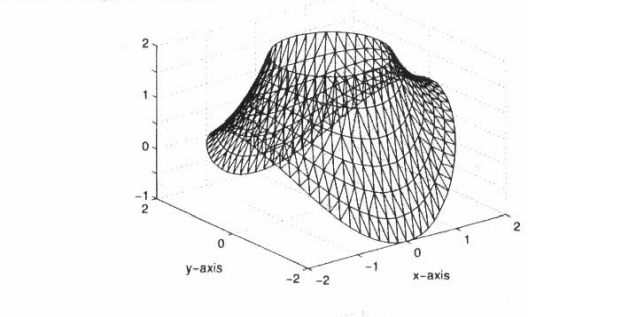
\includegraphics[width=0.9\linewidth]{24}
	\centering
	\label{pfig:ch13_24}
\end{figure}
	\begin{figure}[H]
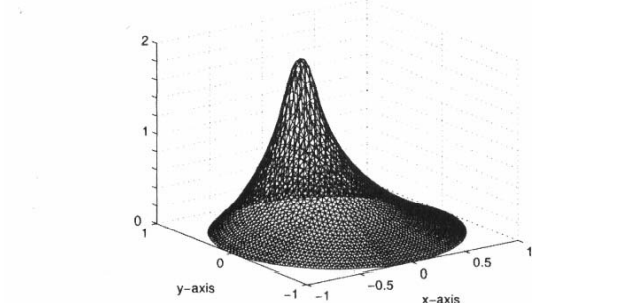
\includegraphics[width=0.9\linewidth]{25}
	\centering
	\label{pfig:ch13_25}
\end{figure}
\textbf{FIGURE 13.39}: (a) (top) Plot of the FEM solution to the BVP of Exercise for the Reader 
13.11. (b) (bottom) Plot of the FEM solution to the BVP of Exercise for the Reader 
13.12(a).
\\
\\
(b) The triangulation of part (a) was rather uniform and had 1795 nodes. In this part we try to work with a smaller number of nodes but deploy them in a strategy that concentrates more of them near where the inhomogeneity $f(x, y)$ has most of its action. Construct a triangulation using between 500 to 1000 nodes and distributed in the four subregions of Figure $13.40$ (a) as follows: Roughly $50 \%$ of the nodes are to be deployed in $\Omega_{1}, 25 \%$ in $\Omega_{2}, 15 \%$ in $\Omega_{3}$, and only $10 \%$ in $\Omega_{4}$. Each of these regions is simply the intersection of the whole domain with the insides of the circles with center $(0,1 / 2)$ having radii: $1 / 4,1 / 2,1$, and $3 / 2$,respectively. The distribution should be more or less uniform in each subregion. 
Obtain and plot the FEM solution. Your solution should look something like the 
one shown in Figure 13.40(c). 
\begin{figure}[H]
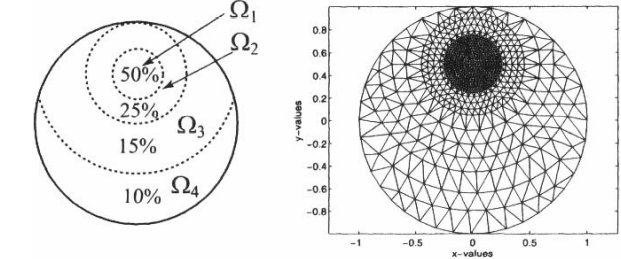
\includegraphics[width=0.9\linewidth]{26}
	\centering
	\label{pfig:ch13_26}
\end{figure}
	\begin{figure}[H]
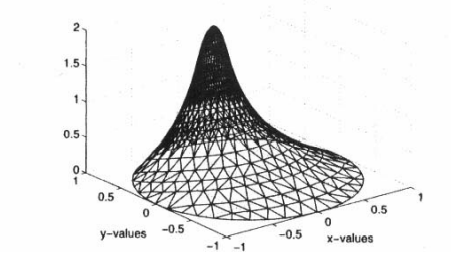
\includegraphics[width=0.9\linewidth]{27}
	\centering
	\label{pfig:ch13_27}
\end{figure}
\textbf{FIGURE 13.40:} (a) (left) Diagram for node deployment strategy of part (b) in Exercise for the Reader 13.12. The unit disk $\Omega$ is split up into four subregions: $\Omega_{1}, \Omega_{2}, \Omega_{3}$, and $\Omega_{4}$.
(b) (top right) A corresponding triangulation.
(c) (bottom) The corresponding FEM solution; it appears graphically indistinguishable from the one obtained in part (a).
\\
\\
\\
We now move on to describe the FEM for the general case of the BVP (10):
$$
\left\{\begin{aligned}
(\mathrm{PDE})-\nabla \cdot(p \nabla u)+q u &=f & & \text { on } \Omega \\
(\mathrm{BCs}) & & \text { on } \Gamma_{1} \\
\vec{n} \cdot \nabla u+r u &=h & & \text { on } \Gamma_{2}
\end{aligned}\right.
$$
Under the assumptions indicated in the theoretical discussion earlier in this 
section, this BVP can be shown to be equivalent to the following minimization 
problem: 
\\
\\
Minimize the functional: 
\begin{equation}
F[u]=\iint_{\Omega}\left[\frac{1}{2} p u_{x}^{2}+\frac{1}{2} p u_{y}^{2}+\frac{1}{2} q u^{2}-f u\right] d x d y+\int_{r_{2}}\left[\frac{1}{2} r u^{2}-h u\right] d s
\end{equation}
over the following set of admissible functions: 
\begin{equation}
A=\left\{v: \Omega \rightarrow \mathbb{R}: v(x)\right. is~ continuous,
\end{equation}
$$ v^{\prime}(x) ~is~piecewise~continuous~and~ bounded,~and~ v(x, y)=g(x, y) ~on~ \left.\Gamma_{1}\right\}.$$
\\
Note that the class of admissible functions requires only the Dirichlet boundary conditions (on $\Gamma_{1}$ ). The Robin boundary conditions (on $\Gamma_{2}$ ), are accounted for in the functional (26) and will be automatically satisfied by the solution.
\\
\\
Analogous to the one-dimensional method presented in Section 10.5, the FEM will solve a corresponding finite-dimensional minimization problem where the functional $F[u]$ of (26) is kept the same, but the set of admissible functions is reduced to an approximating smaller set determined by the basis functions of the triangulation. Thus we will be looking for minimizers of the functional $F$ among functions of the form $v=\sum_{i=1}^{m} c_{i} \Phi_{i}$, where the $\Phi_{i}=\Phi_{i}(x, y)$ are the basis functions.\\
The basis functions corresponding to nodes on the boundary portion $\Gamma_{1}$ will have their coefficients determined by the Dirichlet boundary conditions; it is the remaining coefficients (corresponding to interior nodes and nodes on the boundary portion $\Gamma_{2}$ ) that need to be determined. We now briefly outline the FEM for this general BVP. We follow this outline with some additional details and then give examples.
\\
\\
\textbf{FEM FOR THE BVP (10)-GENERAL CASE:}\\
\\
\textbf{Step $\#1$: Decompose the domain into elements, and represent the set of nodes and elements using matrices. Separate the nodes $N_{i}$ into the internal nodes and non-Dirichlet boundary nodes: $N_{1}, N_{2}, \cdots, N_{n}$ (that lie in $\Omega \cup \Gamma_{2}$ ), and the Dirichlet boundary nodes $N_{n+1}, N_{n+2}, \cdots, N_{m}$ (that lie on $\Gamma_{1}$ ). Denote the basis function $\Phi_{N_{i}}$ corresponding to node $N_{i}$ simply by $\Phi_{i}$. It is important that nodes be placed at all endpoints (interfaces) of $\Gamma_{1} / \Gamma_{2}$ and that these endpoints be counted as Dirichlet boundary nodes (i.e., grouped with those in $\left.\Gamma_{1}\right)$.}
\\
\\
\textbf{Step $\#2$: Use the Dirichlet BCs $u(x, y)=g(x, y)$ on $\Gamma_{1}$ to determine the coefficients of the Dirichlet boundary node basis functions of an admissible function: $v=\sum_{i=1}^{m} c_{i} \Phi_{i}$, i.e., $c_{i}=g\left(N_{i}\right)$ for each $i=n+1, n+2, \cdots, m$.}
\\
\\
\textbf{Step $\#3$: Assemble the $\boldsymbol{n} \times \boldsymbol{n}$ stiffness matrix $A$ and load vector b needed to determine the remaining coefficients $c_{1}, c_{2}, \cdots, c_{n}$ which work to solve the discrete minimization problem corresponding to the BVP.
\\
\\
Step $\#4$: Solve the stiffness equation $A c=b$, and obtain the FEM solution}
$$
v=\sum_{i=1}^{m} c_{i} \Phi_{i} .
$$
As before, the coefficients $c_{1}, c_{2}, \cdots, c_{n}$ will eventually be determined as the solution vector $c=\left[\begin{array}{llll}c_{1} & c_{2} & \cdots & c_{n}\end{array}\right]^{\prime}$ of a linear system (14) $A c=b$. The stiffness matrix $A$ and load vector $b$ will, in general, have entries given as follows:
\begin{equation}
a_{i j}=\iint_{\Omega}\left[p \nabla \Phi_{i} \cdot \nabla \Phi_{j}+q \Phi_{i} \Phi_{j}\right] d x d y+\int_{\Gamma_{2}} r \Phi_{i} \Phi_{j} d s(1 \leq i, j \leq n)
\end{equation}
and
\begin{equation}
\begin{aligned}
b_{j} &=\iint_{\Omega} f \Phi_{j} d x d y+\int_{\Gamma_{2}} h \Phi_{j} d s \\
&-\sum_{s=n+1}^{m} c_{s}\left\{\iint_{\Omega}\left[p \nabla \Phi_{s} \cdot \nabla \Phi_{j}+q \Phi_{s} \Phi_{j}\right] d x d y+\int_{\Gamma_{2}} r \Phi_{s} \Phi_{j} d s\right\}(1 \leq j \leq n) .
\end{aligned}
\end{equation}
In these formulas the integrals over $\Gamma_{2}$ are with respect to arclength (i.e., positively oriented line integrals). These can be derived in a similar fashion to what was done in the purely Dirichlet $\mathrm{BC}$ case (see the development of (13)). As before, we observe that the stiffness matrix is a symmetric matrix. The timeconsuming part of the FEM is still the assembly process. The mechanics are as in the purely Dirichlet case (just replace $\left(15^{\ell}\right)$ and $\left(16^{\ell}\right)$ with their analogs for (28) and (29)).
\\
\\
The assembly process can be coded much like the way we did it for Example 13.7. The only new feature here is the presence of the line integrals. Before entering into the MATLAB code, we give a brief outline of how such line integrals can be evaluated. We show how to numerically evaluate integrals of the form $\int_{\Gamma_{2} \cap r_{1}} F d s$, where $F$ is any function on $\Gamma_{2}$ in the setting of an assembly code. Any such integral can be broken up into a sum of corresponding integrals over line segments. Let $L$ denote a typical such line segment, connecting nodes $N_{1}$ and $N_{2}$ of $T_{\ell}$. Letting $\vec{v}=N_{2}-N_{1}$, we can write:
\begin{equation}
\int_{L} F d s=\int_{0}^{1} F\left(N_{1}+s \vec{v}\right)\|\vec{v}\| d s
\end{equation}
from the definition of line integrals. Such integrals could be done with 
MATLAB's \texttt{quad} (or \texttt{quadl})-but in a general FEM code, it would be awkward to combine the M-files for the integrand "F" with the needed change in variables 
unless we resort to symbolic variables. We avoid this dilemma and maintain 
consistency with the recommended method for approximating double integrals by 
invoking the following numerical quadrature approximation for ordinary integrals:
\begin{equation}
\int_{0}^{1} f(x) d x \approx(1 / 6)\{f(0)+4 f(1 / 2)+f(1)\}
\end{equation}
This formula, known as the \textbf{Newton-Coates formula} with three equally spaced 
points, is exact for polynomials up to degree three (Exercise 24). For more on 
such one-dimensional quadrature formulas, see Chapter 5 of [ZiMo-83], or see any 
good book on numerical analysis. What is most pertinent is that the accuracy of 
this approximation makes it feasible to use in the FEM; the underlying theory can 
be found in the references mentioned above. Combining (30) and (31) yields the 
following quadrature approximation, which is easily incorporated in FEM codes: 
\begin{equation}
\int_{L} F d s \approx\left(\left\|N_{1}-N_{2}\right\| / 6\right)\left\{F\left(N_{1}\right)+4 F\left(\left[N_{1}+N_{2}\right] / 2\right)+F\left(N_{2}\right)\right\}
\end{equation}
EXERCISE FOR THE READER 13.13: (a) Write an M-file \texttt{lineint = bdyintapprox(fun, tri, redges)} that works as follows: The inputs will be fun, an inline (or M-file) function of the variables $x$ and $y$, a $3 \times 2$ matrix \texttt{tri} of nodes of a triangle in the plane, and a 2-column matrix \texttt{redges}, possibly empty ([]). The rows of \texttt{redges} consist of the corresponding increasing node indices (from 1 to 3 corresponding to their row in \texttt{tri}) of nodes that are endpoints of segments of the triangle that are part of the "Robin" boundary (for an underlying FEM problem). Thus the rows of \texttt{redges} can include only the following three vectors: $\left[\begin{array}{ll}1 & 2\end{array}\right],\left[\begin{array}{ll}1 & 3\end{array}\right]$, and $\left[\begin{array}{ll}2 & 3\end{array}\right]$. The output, \texttt{lineint}, will be the approximation of the corresponding line integral of \texttt{fun} over the Robin segments of the triangle, by using formula $(32)$.
(b) Test the accuracy of your $M$-file in computing the following line integrals over the indicated edge sets of the triangle with vertices $N_{1}=(0,0), N_{2}=$ $(2,0), \quad N_{3}=(0,3)$, and then on the triangle with vertices $N_{1}=(0,0), N_{2}=(.2,0)$, $N_{3}=(0, .3)$. In the notation used below, $\varepsilon_{i j}$ denotes the edge of this triangle joining $N_{i}$ to $N_{j}(i \neq j)$. The line integrals are given below for the larger triangle:
$$\int_{\epsilon_{12} \cup \epsilon_{21}} 4 d s=8+4 \sqrt{13}, \int_{\epsilon_{12} \cup \varepsilon_{13}} \cos (\pi x / 4+\pi y / 2) d s=2 / \pi .
$$
In our next example, we will solve a BVP over an odd-shaped region. The 
problem is carefully constructed so that the exact solution will be available for 
comparison purposes. In Exercise for the Reader 13.14, the reader will be asked to 
solve another such problem on the same region for which an exact solution is not 
available. 
\\
\\
\textbf{EXAMPLE 13.8:} Use the finite element method to solve the following mixed BVP over the parabolically shaped domain $\Omega=\{(x, y): 0 \leq x \leq 10,0 \leq y$ $\leq x(10-x)\}$
$$
\left\{\begin{array}{l}
(\mathrm{PDE}) \quad-\Delta u=-1 / 25 \quad \text { on } \Omega \\
(\mathrm{BCs}) \quad \begin{array}{c}
u=0 ~~~~on~ x-aris\\
\vec{n} \cdot \nabla u=\frac{y}{25\left(101-40 x+4 x^{2}\right)^{1 / 2}}
\end{array} \text { on } y=x(10-x)
\end{array}\right.
$$
(a) Use first a triangulation with between 300 and 500 nodes that are more or less uniformly distributed. Compare with the exact solution $u(x, y)=y^{2} / 50$.\\
(b) Repeat part (a) this time using a similar triangulation with between 1000 and 2000 nodes.
\\
\\
Before we begin to solve this example, we leave the reader to perform the following:
\\
\\
EXERCISE FOR THE READER 13.14: Verify that the exact solution provided really solves the $B V P$ in the above example.
\\
\\
SOLUTION TO EXAMPLE 13.8: Part (a): To decide on the linear gap distance 
between nodes, we first find the area of $\omega$: 
$$
\operatorname{area}(\Omega)=\int_{0}^{10} x(10-x) d x=\left[5 x^{2}-x^{3} / 3\right]_{0}^{10}=500 / 3
$$
If we place the nodes in small square configurations (cf. Method 1 of Example $13.2(\mathrm{a})$ ), then, roughly, each node would account for an area $\delta^{2}$. Thus, if $m$ denotes the number of nodes we use, then we would have (approximately) $m \delta^{2} \approx \operatorname{area}(\Omega)$, the left side being a bit larger due to boundary nodes. This gives the estimate
\\
\begin{equation}
\delta \approx \sqrt{\operatorname{area}(\Omega) / m}
\end{equation}
\\
for the gap size we should use if we want to deploy $m$ nodes. This formula can be used in the creation of squarelike nodegrids on any two-dimensional region with smooth boundary curves. Using ( 33 ) with the above area and $m=350$, we arrive at the value $\delta=\sqrt{500 / 3 / 350 }\approx 0.6901 \ldots .$
\\
\\
We begin by using MATLAB to deploy nodes in the interior of $\Omega$, maintaining a safe distance close to $\delta$ away from the boundary and placing them in a square grid configuration with sidelength $\delta$ :
\\
\\
\texttt{>> bdyf= inline('x.*(10-x)') ;}
\texttt{>> delta=sqrt(500/3/350);}
\texttt{>> nodecount=l;}
\texttt{>> for i=l:10/delta}
\texttt{for j=l:bdyf(i*delta)/delta}

~\texttt{xtemp=i*delta; ytemp=j*delta;}

~\texttt{if (bdyf(xtemp-delta/2)>ytemp)\&... }

~\texttt{(bdyf(xtemp)>ytemp+delta/2)\&(bdyf(xtemp+delta/2)>ytemp) }\\
\texttt{\%These conditions assure that the parabolic portion of the boundary}\\
\texttt{\%does not get too close to the candidate (xtemp, y temp) for an}\\
\texttt{\%internal node.}

~\texttt{x(nodecount)=xtemp; y (nodecount)=ytemp; }
`
~\texttt{nodecount = nodecount+1; }


~\texttt{end}\\
\texttt{end}\\
\texttt{end}\\
\\
We would like to assign the boundary nodes in such a way that the distance gap between nodes is approximately $\delta$. This is quite simple to do on the straight portion of the boundary. For the curved portion, we now introduce a general method to accomplish such node deployment. Recall, the arclength formula for the graph of a function $f(x)$ over an interval $[a, b]: L=\int_{a}^{b} \sqrt{1+\left[f^{\prime}(x)\right]^{2}} d x$. Now the parabolic boundary graph function has $f^{\prime}(x)=10-2 x$ so that the largest that the integrand $\sqrt{1+\left[f^{\prime}(x)\right]^{2}}$ will be over $[0,10]$ is $\sqrt{101} \approx 10$. (This maximum change in arclength occurs near the endpoints where the parabola is most steep.) Since we will place a node on the parabola at $x=0, y=0$ (call this the "most recent node"), and then continue advancing $x$ by $\delta / 3 \cdot 10$ (so the corresponding arclength of the parabola will advance by no more than about $\delta / 3$ ), as soon as the arclength from the most recent node exceeds $\delta$, we create a new node. Since we will place a node also at $(10,0)$, we will place a safeguard to prevent the nodes on the parabola from getting too close to this one. The code below is set up so that the Dirichlet nodes are indexed last.
\\
\\
\texttt{>> arcint = inline('sqrt(101-40*x+4*x. 2)'); }\\
\texttt{>> xrefl=0; xref2=delta/30; cumlen=quad(arcint,xrefl,xref2); 
}\\
\texttt{>> while xrefKlO}\\
\texttt{while cumlen<delta}

\texttt{xref2=xref2+delta/30;;}

\texttt{cumien=quad(arcint,xref1,xref2); 
}\\
\texttt{end}\\
\texttt{if xref2<10-delta/40 
}

~\texttt{x(nodecount)=xref2; y (nodecount)=bdyf(xref2) ;}

~\texttt{nodecount = nodecount+1;}

\texttt{end}

\texttt{xrefl=xref2; xref2=xref2+delta/30;}

\texttt{cumlen=quad(arcint,xrefl,xref2); 
}\\
\texttt{end}\\
\texttt{if quad(arcint,xrefl,10)>delta/2}

\texttt{nodecount = nodecount+1;}\\
\texttt{end}\\
\texttt{>> x(nodecount)=10; y(nodecount)=0; 
}\\
\texttt{>> nodecount = nodecount+1; }\\
\texttt{>> \%finally put nodes on interior of horizontal segment}\\
\texttt{>> num = floor(10/delta); delta2=10/num; xref=10-delta2;}\\
\texttt{>> while xref>delta2/4 }

~\texttt{(xnodecount)=xref; y(nodecount)=0; 
}

~\texttt{nodecount - nodecount+1; xref=xref-delta2; }\\
\texttt{end}\\
\texttt{>> x (nodecount) =0; y (nodecount) =0; \%last node}\\
\texttt{>> nodecount = nodecount+1; tri=delaunay(x,y); }\\
\texttt{>> trimesh(tri,x,y), axis('equal ) \%Plots the triangulation }
\\
\\
The triangulation is shown in Figure 13.41(a). From the way the nodes were 
constructed, the boundary nodes come after the interior nodes and the first 
boundary node is on the parabolic portion of the boundary. We can thus find the 
key indices by: 
\\
\\
\texttt{>> nint=min (f ind(abs (y-bdyf(x) )<10*eps))-1 \% number of interior nodes}\\
\texttt{$\rightarrow$ nint = 307}
\texttt{>> n=find(x==10\&y==0)-1 \% number of interior/Robin node-:;}\\
\texttt{$\rightarrow$ n = 373}\\
\texttt{>> m=length(x) \% number of nodes }\\
\texttt{$\rightarrow$ m = 388}\\
\texttt{>> size(tri)}\\
\texttt{$\rightarrow$ ans= 693 3 (So there are 693 elements.) }
\\
\\
We give special names to the node numbers of the endpoints of the segment 
(interface with Robin/Dirichlet nodes):
\\
\\
\texttt{>> dirl = m; \%node (0,0)} \\
\texttt{>> dir2 = nint + 1; '>>node (10,0)}\\
\begin{figure}[H]
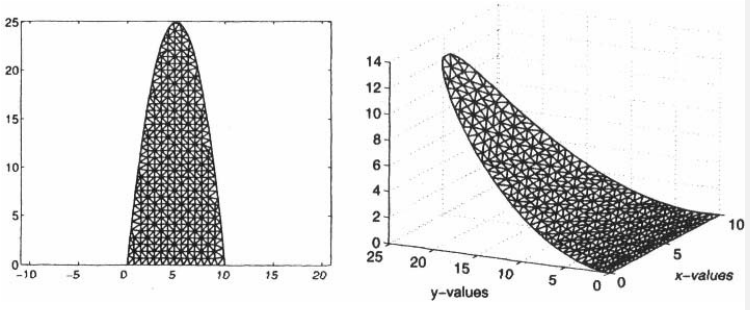
\includegraphics[width=0.9\linewidth]{28}
	\centering
	\label{pfig:ch13_28}
\end{figure}
\textbf{FIGURE 13.41:} (a) (left) The` triangulation of the parabolic region for the BVP of Example 13.8(a). There are 388 nodes and 693 elements. With this resolution the curved boundary is rather well represented by the element boundaries, except near the top where the curvature of the parabola is most extreme. (b) (right) The FEM solution of Example 13.8(a). The exact solution is graphically indistinguishable, the maximum relative error being less than $1 \%$.
\\
\\
\\
From the key node indices found above, we conclude: 
\\
\\
Interior nodes: 1:307 \\
Robin nodes (on interior of parabola): 308: 373\\ 
Dirichlet nodes (on line segment): 374:388\\
\\
Notice we have created nodes at the interfaces of the two boundary portions 
(Dirichlet meets Robin) and these interface nodes will be assigned the Dirichlet 
conditions, as required. Since the Dirichlet boundary conditions are zero, simply 
creating a 388-length vector c of zeros will take care of assigning the Dirichlet 
nodes their appropriate values:
\\
\\
\texttt{>> c= zeros(m,1); }
\\
\\
The crucial index here is $n=373$, the number of interior nodes added to the number of Robin boundary nodes; this is how many coefficients need to be determined, Since, in (10), we have $p \equiv 1, q \equiv 0, f=-1 / 25, g \equiv 0, r \equiv 0$, and since $c_{s}=0(s>n)$, the element matrix analogues of (28) and (29) (cf. ($15^{\ell}$ ) and $\left.\left(16^{\ell}\right)\right)$ are as follows:
\\
\\
$$
a_{\alpha \beta}^{\prime}=\iint_{T_{l}}\left[\nabla \Phi_{i_{\alpha}} \cdot \nabla \Phi_{i_{\beta}}\right] d x d y \quad(1 \leq \alpha, \beta \leq 3)
$$
and
$$
b_{\alpha}^{\ell}=(-1 / 25) \iint_{T_{t}}\left(\Phi_{i_{\alpha}}\right) d x d y+\int_{\Gamma_{2} \cap T_{t}} h(x, y) \Phi_{i_{\alpha}} d s \quad(1 \leq \alpha \leq 3),
$$
where $h(x, y)=\frac{y}{25\left(101-40 x+4 x^{2}\right)^{1 / 2}}$
\\
\\
For each element index $\ell$, these coefficients need to be computed only when the nodes $i_{\alpha}$ and/or $i_{\beta}$ are interior or Robin nodes (i.e., $i_{\alpha}, i_{\beta} \leq n \equiv 373$ ) corresponding to vertices of the corresponding element. The assembly code will invoke the M-file gaussianintapprox of Exercise for the Reader $13.10$ for approximating the double integrals, and the $M$-file robinbdyint of Exercise for the Reader $13.13$ for numerically evaluating line integrals. Here is the assembly code:
\\
\\
\texttt{N=[x y']; E=tri; A=zeros(n); b=zeros(n,1); [L cL]=size(E); }\\
\texttt{for ell=l:L }

~\texttt{nodes=E (ell, :) ; \% global node indices of element}

~\texttt{intnodes=nodes(find(nodes<=n)); \%global interior/Robin node indices}
\texttt{\% find coefficients [a b c] of local basis functions }\\
\texttt{ \% ax + by + c; for int/robin nodes 
}

~\texttt{for i=l:length(intnodes) }

~~\texttt{xyt=N(intnodes(i), :) ; \%main node for local basis function }

~~\texttt{onodes=setdiff(nodes,intnodes(i));}\\
\texttt{\%global indices for two other nodes (w/ zero values) for local basis}\\
\texttt{\%function}

~\texttt{xyr=N(onodes(1),:); }

~\texttt{xys=N(onodes(2), :) ;}

~\texttt{M=[xyr l;xys l;xyt 1]; \% matrix M of (4)}\\
\texttt{\%local basis function coefficients using (6B)}

~\texttt{abccoeff=[xyr(2)-xys(2);xys(1)-xyr(1);xyr(1)*xys(2)-}\\
\texttt{xys(l)*xyr(2) ]/...}

~\texttt{det(M);}

~\texttt{intgrad(i,:)=abccoeff(1:2) ' ;}

~\texttt{abe(i,:)=abccoeff;}\\
\texttt{end}
\\
\\
\texttt{ determine if there are any Robin edges}\\
\texttt{marker=0; \%will change to 1 if there are Robin edges.}\\
\texttt{roblocind=find(nodes==dirl|nodes==dir2|(nodes<=n\& nodes >-(nint+1)));}\\
\texttt{\% local indices of nodes for possible robin edges}\\
\texttt{if length(roblocind)>1 
}

~\texttt{elemnodes = N(nodes,:); 
}\\
\texttt{\%now find robin edges and make a 2 column matrix out of their local}\\
\texttt{\%indices. }

~\texttt{rnodes=nodes(roblocind); \%global indices of robin nodes}

~\texttt{count=l;}

~\texttt{for k=(nint+1):n}

~~\texttt{if ismember(k,modes) \& ismember (k+1, rnodes) }

~~~\texttt{robedges(count,:)=[find(nodes==k ) find(nodes==k+l)]; }

~~~\texttt{count=count+l; marker =1;}

~~\texttt{end}\\
\texttt{end}\\
\texttt{end}
\\
\\
\texttt{\% update load vector }\\
\texttt{for il=l:length(intnodes) }

~\texttt{ail = num2str(abc(il, 1) , 10); }

~\texttt{bil = nun2str(abc(il,2) ,10);}

~\texttt{cil = num2str(abc(il,3),10) ;}

~\texttt{fun=inline([ail,'*x+',bil, '*y+', cil],'x','y'); }

~\texttt{integ=-l/25*gaussianintapprox(fun,xyt,xyr,xys); 
}

~\texttt{b(intnodes(il))=b(intnodes(il))+integ; }

~\texttt{\%now add Robin portion, if applicable 
}

~\texttt{\%robin edges were computed above 
}

~\texttt{if marker==l 
}\\
\texttt{prod=inline(['y./(25.*sqrt(101-}\\
\texttt{40.*x+4.*x.2) ) ','* (',ali,'*x+',bil,...)}

\texttt{*y+, cil,')'], 'x','y'); }\\
\texttt{b(intnodes(il))=b(intnodes(il))+bdyintapprox(prod, elemnodes,...}\\
\texttt{robedges);}\\
\texttt{end}\\
\texttt{end}\\
\texttt{clear roblocind modes robedges}\\
\texttt{end}\\
\texttt{A=A+A'-A.*eye(n); \%Use symmetry to fill in remaining entries of A. }
\\
\\
\texttt{sol=A/b; c(l:n)=sol'; c(n+l:m)=0;}
\\
\\
\texttt{\%The result is now easily plotted using the ' trimesh function of the}
\texttt{\%last section:}\\
\\
\texttt{x=N(:,1); y=N (:,2) ; 
}\\
\texttt{trimesh(E,x,y,c), hidden off}\\
\texttt{xlabel('x-axis'), ylabel('y-axis') 
}\\
\\
The following commands will plot the error using the exact solution provided. 
The result is shown in Figure 13.42(a)
\texttt{cexact = zeros(m,l); }\\
\texttt{for i=l:length(x),cexact(i)=y(i) 2/50; end }\\
\texttt{trimesh(E,x,y,abs(c-cexact)) 
}\\
\\
Part (b) is done in exactly the same fashion. In fact, the above code is designed in 
such a way that only the second line (defining delta) in the node deployment needs 
to be adjusted (change 350 to 1800). With this change, the above code will 
produce a numerical solution with error plot shown in Figure 13.42(b).$^{16}$\footnotetext[16]{
 For the convenience of the reader, the entire MATLAB codes for this example (and other longer 
examples and exercises for the reader of this chapter) are included as downloadable text files on the ftp 
site for this book (see the preface for the URL of this ftp site). These codes can easily be pasted 
directly into the MATLAB window, and they can be modified to solve other FEM problems. }
\\

The various examples done so far contain all of the necessary techniques needed 
to apply the FEM to general BVPs of form (10). The next two exercises for the 
reader contain two more examples. 
\\
\\
EXERCISE FOR THE READER 13.15: Consider the following steady-state heat distribution problem on the parabolic region $\Omega=\{(x, y): 0 \leq x \leq 10,0 \leq y$ $\leq x(x-10)\}$ of the preceding example:
$$
\left\{\begin{array}{ccl}
(\mathrm{PDE}) & -\Delta u=f & \text { on } \Omega \\
(\mathrm{BCs}) & u=0 & \text { on } x \text {-axis } \\
& \vec{n} \cdot \nabla u+2 u=40 & \text { on } y=x(10-x)
\end{array}\right.
$$
where the source function is given by: $f(x, y)= \begin{cases}200, & \text { if } 4 \leq x \leq 6 \text { and } 10 \leq y \leq 15 \\ 0, & \text { otherwise. }\end{cases}$
\\
\\
The region $\omega$ along with the boundary conditions and the support of the source 
function / is illustrated in Figure 13.43(a). 
(a) Compute and plot the numerical solution of this BVP using the triangulation of 
the solution to part (a) of Example 13.8. 
\\
\\
(b) Compute and plot the numerical solution of this BVP using the triangulation of 
the solution to Part (b) of Example 13.8. Your plot should look like the one in 
Figure 13.43(b). 
\begin{figure}[H]
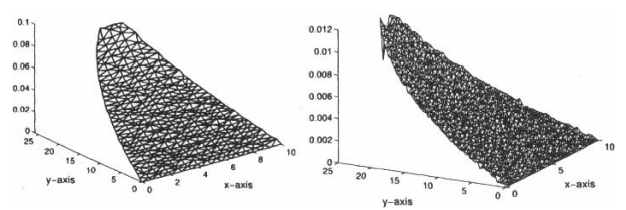
\includegraphics[width=0.9\linewidth]{29}
	\centering
	\label{pfig:ch13_29}
\end{figure}
\textbf{FIGURE 13.42:} Error plots for the FEM solution of Example 13.8. (a) (left) Using the 
triangulation of part (a), which had 693 elements, the actual error was less than 1\%. (b) 
(right) Using the triangulation of part (b), which had 3587 elements, the actual error was 
less than 0.1\%. 
\begin{figure}[H]
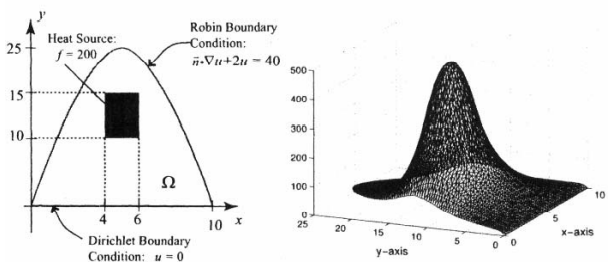
\includegraphics[width=0.9\linewidth]{30}
	\centering
	\label{pfig:ch13_30}
\end{figure}
\textbf{FIGURE 13.43:}domain and boundary conditions for the 
steady-state heat distribution problem of Exercise for the Reader 13.15. The parabolically 
shaped plate has an internal rectangular heat source (temperature = 200) shown by a dark 
rectangle. The bottom (flat) edge is maintained at temperature 0 and the curved part of the 
boundary has a Robin boundary condition, (b) (right) An FEM solution of this problem. 
\\
\\
EXERCISE FOR THE READER 13.16: (a) Contract a squarelike grid and then a 
corresponding triangulation with between 2000 and 3000 nodes for the domain of 
Figure 13.44(a). 
\\
(b) Use the FEM with your triangulation to solve the Laplace problem Aw = 0 on 
this domain with boundary conditions as shown in Figure 13.44(a) and then plot 
your solution. Your plot should look like the one shown in Figure 13.43(b). 
\begin{figure}[H]
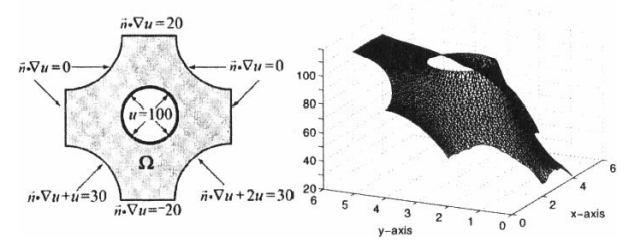
\includegraphics[width=0.9\linewidth]{31}
	\centering
	\label{pfig:ch13_31}
\end{figure}
\textbf{FIGURE 13.44:} (a) (left) Illustration of the domain and boundary conditions for the BVP 
problem of Exercise for the Reader 13.16. The circular (inner) boundary portion has 
Dirichlet boundary conditions; the remaining (outer) boundary portions have the indicated 
Neumann or Robin conditions, (b) (right) Plot of the FEM solution for the Laplace problem 
having the indicated boundary data of (a). The triangulation used had 2655 nodes and 
5024 elements. 
\\
\\
\line(2,0){\textwidth}
\\
\textbf{EXERCISES 13.3}
\begin{enumerate}
	\item (a) Using the exact method of Example 13.5 (with Exercise for the Reader 13.4), solve the 
following BVP on the same hexagonal domain and triangulation ofthat example: 
$$
\left\{\begin{array}{lll}
(\mathrm{PDE}) & -\Delta u=0 & \text { on } \Omega \\
(\mathrm{BC}) & u=x+y & \text { on } \partial \Omega^{\prime}
\end{array}\right.
$$
and plot the resulting numerical solution.
(b) Check that $u(x, y)=x+y$ is the exact solution of the BVP; compare the numerical solution with this exact solution.
	\item (a) Using the exact method of Example 13.5 (with Exercise for the Reader 13.4), solve the 
following BVP on the same hexagonal domain and triangulation ofthat example: 
$$
\left\{\begin{array}{lll}
(\mathrm{PDE}) & -\Delta u=0 & \text { on } \Omega \\
(\mathrm{BC}) & u=x^{2}+y^{2} & \text { on } \partial \Omega^{\prime}
\end{array}\right.
$$
and plot the resulting numerical solution.
\\
(b) Check that $u(x, y)=x^{2}+y^{2}$ is the exact solution of the BVP; compare the numerical solution with this exact solution.
	\item (a) Using the exact method of Example $13.4$ (with Exercise for the Reader 13.4), apply the FEM on the triangular domain $\Omega$ of Figure $13.45$ with the triangulation shown there to solve the following BVP:
	$$
\left\{\begin{array}{lll}
(\mathrm{PDE}) & -\Delta u=2 & \text { on } \Omega \\
(\mathrm{BC}) & u=x & \text { on } \partial \Omega^{\prime}
\end{array}\right.
$$
The vertical/horizontal distance between adjacent nodes is one, and node $\# 7$ has coordinates $(0,0)$ (so, for example, node $\# 1$ is at $(0,3)$ and node $\# 10$ is at $(3,0)$ ). Plot the resulting numerical solution.
(b) Solve this problem again with the FEM but this time use the Gauss quadrature formula (24) (or the \texttt{gaussianintapprox} M-file) to evaluate integrals. Compare with the solution obtained in part (a); comment on any discrepancies or lack thereof. 
(c) Re-solve the problem this time using MATLAB's \texttt{dblquad} d to evaluate all double integrals. 
Compare with the solution obtained in part (a). 
\begin{figure}[H]
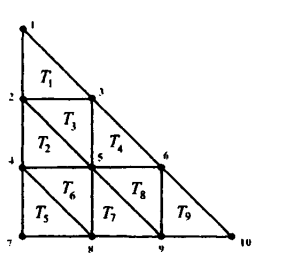
\includegraphics[width=0.7\linewidth]{32}
	\centering
	\label{pfig:ch13_32}
\end{figure}
\textbf{FIGURE 13.45:} Triangular 
domain with basic triangulation 
for Exercise 3. 
	\item Repeat all parts of Exercise 3 for the following BVP on the domain $\Omega$ of Figure 13.45 described 
there.
$$
\left\{\begin{array}{lll}
(\mathrm{PDE}) & -\Delta u=f(x,y) & \text { on } \Omega \\
(\mathrm{BC}) & u=(x+y)^{2} & \text { on } \partial \Omega^{\prime}
\end{array}\right.
where~f(x, y)=\left\{\begin{array}{l}0, \text { if } y \leq 1 \\ 1, \text { if } 1<y \leq 2 \\ 2, \text { if } 2<y\end{array}\right.
$$
	\item Using the same triangulation on the hexagonal domain of Example 13.5, use the FEM to solve 
the following BVP:
$$
\left\{\begin{array}{lll}
(\mathrm{PDE}) & -\Delta u+u=3 & \text { on } \Omega \\
(\mathrm{BC}) & u=x+y & \text { on } \partial \Omega^{\prime}
\end{array}\right.
$$
\textbf{Note:} Since the quadrature formula (24) is exact for polynomials up to second degree, it can be 
used to exactly evaluate all of the integrals that arise. 
	\item Using the same triangulation on the triangular domain of Exercise 3, use the FEM to solve the following BVP:
	$$
\left\{\begin{array}{lll}
(\mathrm{PDE}) & -\Delta u+u=f(x,y) & \text { on } \Omega \\
(\mathrm{BC}) & u=x^{2} & \text { on } \partial \Omega^{\prime}
\end{array}\right.
where~f(x, y)=\left\{\begin{array}{l}0, \text { if } x \leq 1 \\ -2, \text { if } x>1\\\end{array}\right.
$$
\textbf{Note:} Since the quadrature formula (24) is exact for polynomials up to second degree, it can be 
used to exactly evaluate all of the integrals that arise
	\item Consider the Dirichlet problem $(19)$ on the unit disk $\Omega=\left\{(x, y): x^{2}+y^{2}<1\right\}$ :
	$$
\left\{\begin{array}{lll}
(\mathrm{PDE}) & \Delta u=0 & \text { on } \Omega \\
(\mathrm{BC}) & u(1,\theta)=cos^{2}(\theta) & \text { on } \partial \Omega^{\prime}
\end{array}\right.
$$
(a) Use the FEM with the triangulation of part (c) of Example $13.7$ to compute the numerical solution of the problem, performing the double integrals as in Example 13.7. Keep track of the time needed to perform the main assembly (using \texttt{tic...toc}). Use Poisson's integral formula (Theorem 13.1) to compute the "exact solution" to this problem at the nodes of the triangulation and plot solution and the error of the FEM solution obtained.\\
(b) Repeat part (a), but this time use the Gauss quadrature formula (24) (or the \texttt{gaussianintapprox} M-file) to compute the double integrals in the FEM. Compare and contrast the FEM numerical solutions of parts (a) and (b).\\
(c) Use the FEM as in part (b) to find the numerical solution of this problem using a triangulation of the circle having between 3000 and 4000 nodes. Plot the error against the corresponding "exact solution" from Poisson's integral formula.\\
(d) Repeat each of the above parts for the Dirichlet problem identical to the above but with the boundary condition being changed to $u(1, \theta)=\sin ^{2}(\theta / 2)$.
	\item  Consider the following Dirichlet problem (19) on the disk $ \Omega=\left\{(x, y):(x-1)^{2}+(y-3)^{2}<5\right\}$ : 
	$$
\left\{\begin{array}{lll}
(\mathrm{PDE}) & \Delta u=0 & \text { on } \Omega \\
(\mathrm{BC}) & u(x,y)=lnx+2y & \text { on } \partial \Omega^{\prime}
\end{array}\right.
$$
a) Use the FEM with a triangulation having between 500 and 1000 nodes to compute the 
numerical solution of the problem, performing the double integrals as in Example 13.7. Keep 
track of the time needed to perform the main assembly (using \texttt{tic...toc}) . Use Poisson's 
integral formula (Theorem 13.1) to compute the "exact solution" to this problem at the nodes of 
the triangulation and plot solution and the error of the FEM solution obtained. 
\\
(b) Repeat part (a), but this time use the Gauss quadrature formula (24) (or the 
\texttt{gaussianintappro} x M-file) to compute the double integrals in the FEM. Compare and 
contrast the FEM numerical solutions of parts (a) and (b). 
\\
(c) Use the FEM as in part (b) to find the numerical solution of this problem using a triangulation of the circle having between 3000 and 4000 nodes. Plot the error against the corresponding "exact solution" from Poisson's integral formula.
\\
(d) Repeat each of the above parts for the Dirichlet problem identical to the above but with (i) the boundary condition being changed to $u(x, y)=2 x+e^{y}$ and then (ii) with the PDE changed to $-\nabla \cdot\left(e^{x+y} u\right)+u=y$ but all else as in the original problem. 
	\item Consider the following Robin problem for the Laplacian on the unit disk $\Omega={(x, y) : x^{2}+y^{2}<1}$:
	$$
\left\{\begin{array}{lcl}
(\mathrm{PDE}) & \Delta u=0 & \text { on } \Omega \\
(\mathrm{BC}) & \vec{n} \cdot \nabla u+u=3 & \text { on } \partial \Omega
\end{array}\right.
$$
(a) Use the FEM to solve this problem using a triangulation having between 500 to 1000 nodes and plot your numerical solution.\\
(b) Create a triangulation having between 1500 and 2000 nodes containing the node set of your triangulation of part (a). Re-solve the BVP with the FEM on this triangulation. Plot the new solution, compare it with that of part (a), and finally plot the difference of the two solutions on the common node set.\\
(c) Create a triangulation having between 3000 and 3500 nodes containing the node set of your triangulation of part (b). Re-solve the BVP with the FEM on this triangulation. Plot the new solution, compare it with that of part (b), and finally plot the difference of the two solutions on the common node set.\\
(d) Repeat each of parts (a) through (c) for the BVP with the same Robin boundary conditions of the above problem, but with the PDE changed to:\\
(i) $\nabla \cdot\left(e^{x+y} u\right)=0$,
(ii) $\nabla \cdot\left(e^{x+y} u\right)=3$,
(iii) $\nabla \cdot\left(e^{x+y} u\right)=-3$,
(iv) $-\nabla \cdot\left(e^{x+y} u\right)+u=3$

	\item Consider the following BVP on the annulus $\Omega=\left\{(x, y): 1 \leq x^{2}+y^{2} \leq 4\right\}$ of Exercise for the Reader 13.11:
	$$
\left\{\begin{array}{ccc}
(\mathrm{PDE}) & \Delta u=e^{x^{2} / 2} & \text { on } \Omega \\
(\mathrm{BCs}) & \vec{n} \cdot \nabla u \equiv 10 & \text { on } x^{2}+y^{2}=1 \\
& u(2, \theta)=50 & \text { on } x^{2}+y^{2}=4
\end{array}\right.
$$
(a) Use the FEM to solve this problem using a triangulation having 500 to 1000 nodes and plot 
your numerical solution.\\ 
(b) Create a triangulation having between 1500 and 2000 nodes containing the node set of your 
triangulation of part (a). Re-solve the BVP with the FEM on this triangulation. Plot the new 
solution, compare it with that of part (a), and finally plot the difference of the two solutions on 
the common node set. \\
(c) Create a triangulation having between 3000 and 3500 nodes containing the node set of your 
triangulation of part (b). Re-solve the BVP with the FEM on this triangulation. Plot the new 
solution, compare it with that of Part (b), and finally plot the difference of the two solutions on 
the common node set. \\
(d) Repeat each of parts (a) through (c) for the BVP with the same Robin boundary conditions 
of the above problem, but with the PDE changed to: 
(i) $\nabla \cdot\left(e^{x+y} u\right)=0$,
(ii) $\nabla \cdot\left(e^{x+y} u\right)=3$
(iii) $\nabla \cdot\left(e^{x+y} u\right)=-3$
(iv) $\nabla \cdot\left(e^{x+y} u\right)+u=3$
	\item This exercise will use the FEM to solve the heat problem (1) 
	$$
\left\{\begin{array}{l}
\Delta u=0 \text { on } \Omega, u=u(x, y) \\
\partial u / \partial n=0, \text { on outer rectangle } \\
u=40, \text { on small circle, } u=500, \text { on large circle }
\end{array}\right.
$$
from the introductory section. Take the domain (see Figure 13.2) to be the rectangle: $-1<x<0.5,-0.5<y<0.5$ with the following two disks deleted: larger circle: center = $(-0.65,0.15)$, radius $=0.25$ and smaller circle: center $=(0.1,-0.2)$, radius $=0.1$. In each case you are to plot your results.\\
(a) First use a triangulation with between 300 and 500 nodes, more or less uniformly spaced.\\
(b) Repeat part (a) using a triangulation with between 1500 and 2000 nodes.\\
(c) (i) Repeat parts (a) and (b) on the BVP gotten from ( 1 ) by changing the BC on the outer rectangle to be $\partial u / \partial n+u=40$, but keeping all else the same. (ii) Do this again using instead the $\mathrm{BC}$ on the larger circle to be $\partial u / \partial n+4 u=40$. (iii) Repeat using instead the $\mathrm{BC}$ on the larger circle to be $\partial u / \partial n+u=80$.\\
(d) (i) Repeat parts (a) and (b) on the BVP gotten from (1) by changing the PDE to be $\Delta u=f(x, y)$, where $f(x, y)=-100$ on the circle with center center $=(0.3,0.25)$, radius $=0.1$, and $f(x, y)=0$ elsewhere (but keeping all else the same). (ii) Do this again but change the PDE to $\Delta u+2 u=f(x, y)$.
	\item (\textit{Comparison of the FEM and the Finite Difference Method for a Certain Mixed BVP}) (a) Use 
the FEM to solve the BVP of Exercise for the Reader 11.8. For the triangulation, let the node 
set correspond to that in part (a) ofthat exercise for the reader, i.e., nodes are uniformly spaced 
in a squarelike grid with horizontal and vertical gap size equaling h = 0.05. Let MATLAB's 
\texttt{delaunay} produce the actual triangulation once you create the node set. Plot your solution 
and compare it with Figure 11.23(a). Produce also a contour plot for your FEM solution and 
compare it with Figure 11.23(b).\\
(b) Repeat part (a), but using the finer grid with horizontal/vertical gap size h = 0.02. 
	\item Repeat both parts of Exercise 11 on the BVP with the same boundary conditions but with the PDE changed from the Laplace equation to $-\nabla \cdot\left(\left[x^{2}+y^{2}+1\right] u\right)+u=\cos (x y)$.
	\item (\textit{Determination of Maximum Tolerable Heat}) Consider the domain of Figure 13.46: 
	\begin{figure}[H]
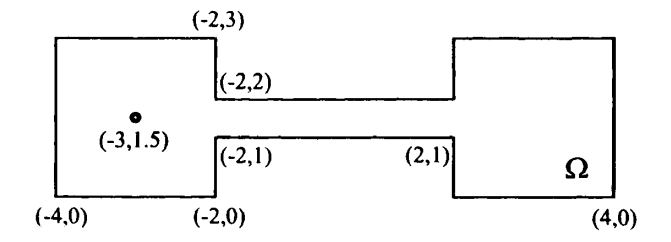
\includegraphics[width=0.9\linewidth]{33}
	\centering
	\label{pfig:ch13_33}
\end{figure}
\textbf{FIGURE 13.46:} A domain consisting of two squares joined by a rectangular neck.
\\
\\

(a) In this domain, an observer at location $(-3,1.5)$ (left side) cannot tolerate a temperature greater than 50 . All edges except for the right edge are kept insultated $\vec{n} \cdot \nabla u=0$ while the right edge will be maintained at a certain temperature $u=T_{\text {hot }}$. What is the maximum value of $T_{\text {hot }}$ so the observer's requirement is met? Try to get your answer accurate to at least two decimals. For the PDE in the domain use the basic Laplace equation $\Delta u=0$.\\
(b) How would the answer in part (a) change if the rectangular length were to be doubled in length?\\
(c) How would the answer in part (a) change if the rectangular length were to have only half of its height?\\
(d) How would the answer in part (a) change if the square on the right were to have its sidelength doubled (but the left square is still kept the same)?\\
(e) How would the answer in part (a) change if the hot edge of the square on the right were the top edge rather than the right edge?
	\item Let $\Omega$ be the domain shown in Figure 13.47, with the deleted disk having center $(2.5,2.5)$ and radius, $0.75$.
(a) Create triangulation of $\Omega$ having between 300 and 400 (essentially equally spaced) nodes.\\
(b) Create a triangulation of $\Omega$ having between 1500 and 2000 nodes.\\
(c) Use the FEM with the triangulation of part (a) to solve the following BVP on $\Omega$ :
$$
\left\{\begin{array}{l}
\Delta u=0 \text { on } \Omega \\
\vec{n} \cdot \nabla u=10, \text { on triangle } \\
\mathbf{u}=100, \text { on circle }
\end{array}\right.
$$
Plot your result and then repeat with the triangulation of part (b).
(d) Repeat part (c) on the modified BVP gotten by changing the PDE to be (i), $-\Delta u=x^{2} / 2$, but  keeping alt else the same; and then to (ii)  $-\Delta u+e^{x / 2} u=x^{2} / 2$
\begin{figure}[H]
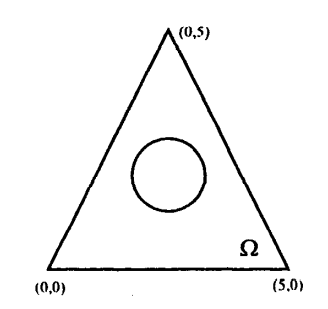
\includegraphics[width=0.5\linewidth]{34}
	\centering
	\label{pfig:ch13_34}
\end{figure}
\textbf{FIGURE 13.47:} Triangular domain  with basic triangulation for Exercise 3. 
	\item 
	(a) Triangulate the domain of Figure $13.48$ using between 400 and 800 nodes, more or less equally spaced.\\
(b) Repeat part (a) but this time use between 2000 and 2500 nodes.\\
(c) Use the FEM and the triangulation of part
(a) to solve the heat problem on the domain of Figure $13.48$ governed by the Laplace equation $\Delta u=0$ and the boundary conditions shown in the figure. Plot your numerical solution.\\
(d) Repeat part (c), this time using the triangulation of part (b).\\
(e) Repeat both parts (c) and (d) on the modified BVP gotten by changing the boundary conditions on $\Gamma_{1}^{2}$ and $\Gamma_{1}^{3}$ to be $\vec{n} \bullet u=0$ (insulated), but keeping all else the same.\\
(f) Repeat both parts (c) and (d) on the modified BVP gotten by changing the boundary conditions on $\Gamma_{1}^{2}$ and $\Gamma_{1}^{3}$ to be the Robin conditions: $\vec{n} \cdot u=20$ and $\vec{n} \cdot u=-20$, respectively, but keeping all else the same.\\
(g) Repeat both parts (c) and (d) on the modified BVP gotten by changing the boundary conditions on $\Gamma_{1}^{2}$ and $\Gamma_{1}^{3}$ to be the Robin conditions: $\vec{n} \cdot u+u=20$ and $\vec{n} \cdot u+u=20$, respectively, but keeping all else the same.\\
(h) Repeat both parts (c) and (d) on the modified BVP gotten by changing the PDE to be $\nabla \cdot\left(\left(\left[2^{x / 2}+y\right] u\right)+u=10\right.$, but keeping all else the same.
\begin{figure}[H]
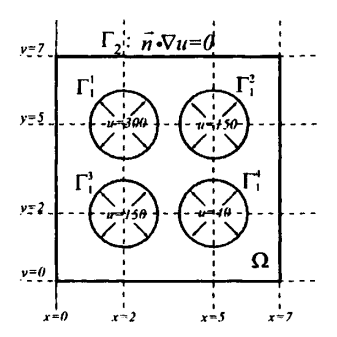
\includegraphics[width=0.5\linewidth]{35}
	\centering
	\label{pfig:ch13_35}
\end{figure}
\textbf{FIGURE 13.48:} Boundary conditions for the heat problem of Exercise 11. The outer square boundary $\Gamma_{2}$ is insulated, while the four circular inner boundary portions $\Gamma_{1}^{i}, 1 \leq i \leq 4$, are each maintained at the indicated temperatures.
	\item Let $\Omega$ be the domain between the $x$-axis and the graph of $y=e^{x}$ from $x=0$ to $x=4$.
(a) For the function $u(x, y)=\sin (x /(y+1))+x^{2} y / 25$, determine functions $g(x), f(x, y)$ and $h(x, y)$ so that $u(x, y)$ solves the following BVP:
	$$
\left\{\begin{array}{lll}
(\mathrm{PDE}) & -\Delta u+u=f(x,y) & \text { on } \Omega \\
(\mathrm{BCs}) & u=g(x)on x-axis; & \vec{n} \cdot \nabla u+u=h(x, y) \text { on curved portion of } \partial \Omega 
\end{array}\right.
$$
(b) Construct a triangularon of ? having between 300 and 500 nodes. Compute the 
corresponding FEM solution and use the exact solution to plot the error.\\ 
(c) Repeat part (b) this time using between 1500 and 2000 nodes. 
	\item Write an M-file, \texttt{integ=quadint (fun, v1, v2, v3, v4)}, whose inputs are fun an inline function of $x, y$, and four $2 \times 1$ matrices \texttt{v1, v2, v3, v4} that are vertices (in any order) of quadrilateral (four sided polygon) in the $x y$-plane. If we denote this quadrilateral by $Q$, the output \texttt{integ} should be the numerical integral $\int_{Q} f u n(x, y) d x d y$, computed using \texttt{dblquad},
\\
\\	
MATLAB's numerical integrator. 
	\item Derive formulas (13) through (18) for the FEM for BVPs with purely Dirichlet BCs. 
	\item (a) Establish the integral formula (21) for general planar regions of Figure 13.34. \\
(b) Derive a similar integration formula for regions between functions of y.\\
\textbf{Suggestion:} For part (a), in the last integral, make the following substitution $y=y$ low $(x)+$ $u(y \operatorname{top}(x)-y \operatorname{low}(x))$.
	\item Suppose that a Gauss quadrature formula (22):
	$$
\int_{T} f(x, y) d x d y \approx w_{1} f\left(\xi_{1}\right)+w_{2} f\left(\xi_{2}\right)+\cdots+w_{n} f\left(\xi_{n}\right)
$$
is exact for polynomials of degree up to p. Use Taylor's theorem in two variables to show that 
if the integrand has continuous partial derivatives up to order p + 1, then the error of the 
approximation (22) is $O(h^{p+1})$
), where A is the diameter of the triangle T
	\item Show that the Gauss quadrature formula (23):
	$$
\int_{T} f(x, y) d x d y \approx \frac{\operatorname{Area}(T)}{3}\left\{f\left(V_{1}\right)+f\left(V_{2}\right)+f\left(V_{3}\right)\right\}
$$
is exact for linear (first-degree) polynomials, but not for quadratic (second degree) polynomials. 
Here, T is a triangle and $V_1, V_2, V_3 $are its vertices.
	\item Show that the Gauss quadrature formula (24): 
	$$
\int_{T} f(x, y) d x d y \approx \frac{\operatorname{Area}(T)}{3}\left\{f\left(\left[V_{1}+V_{2}\right] / 2\right)+f\left(\left[V_{1}+V_{3}\right] / 2\right)+f\left(\left[V_{2}+V_{3}\right] / 2\right)\right\}
$$
is exact for quadratic (second-degree) polynomials. Here, T is a triangle and $V_1, V_2, V_3 $are its 
vertices. \\
\textbf{Suggestion:} First work with the standard triangle with vertices (0,0), (1,0), and (0,1). You 
need only verify it for the basis polynomials and use of linearity. Once this is done use affine 
maps to get the result for general triangles (see Exercise 19 of the previous section).
	\item Show that the Newton-Coates quadrature formula (30): 
	$$
\int_{0}^{1} f(x) d x \approx(1 / 6)\{f(0)+4 f(1 / 2)+f(1)\}
$$
is exact when f(x) is polynomial of degree at most three. 
	\item[NOTE:]The next four exercises will introduce the reader to some refinement and adaptive 
implementations of the FEM. These are based on the simple refinement scheme of splitting an element 
into four similar elements by introducing a new node at the midpoint of each edge; see Figure 13.49. 
\begin{figure}[H]
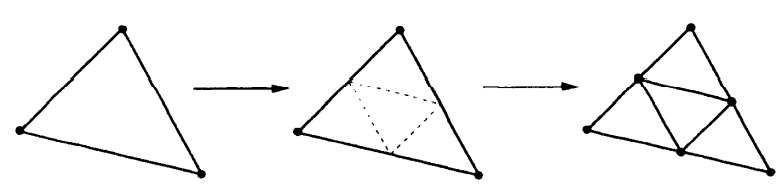
\includegraphics[width=0.9\linewidth]{36}
	\centering
	\label{pfig:ch13_36}
\end{figure}
\textbf{FIGURE 13.49:} A refinement scheme for triangular meshes that is easily programmed into FEM 
routines. 
	\item 25. uzupelnic
	\item (Examples of FEM with Mesh Refinement) (a) For the BVP of Example 13.5, set up MATLAB code to perform the FEM starting with the triangulation of that example, and then after refining the triangulation (as in Exercise 25), re-solving the problem on the new triangulation and looking at the absolute value of the difference of the new FEM solution with the previous FEM solution (on the previous grid). Continue to iterate this process until the absolute value of the difference is less than le-4 or the FEM calculations take more than a few minutes, whichever happens first. Plot the successive FEM solutions as well as the difference graphs.\\
(b) Repeat the instructions of part (a) on the BVP of Exercise 2; compare the final FEM (Examples of FEM with Mesh Refinement) (a) For the BVP of Example 13.5, set up MATLAB code to perform the FEM starting with the triangulation of that example, and then after refining the triangulation (as in Exercise 25), re-solving the problem on the new triangulation and looking at the absolute value of the difference of the new FEM solution with the previous FEM solution (on the previous grid). Continue to iterate this process until the absolute value of the difference is less than le-4 or the FEM calculations take more than a few minutes, whichever happens first. Plot the successive FEM solutions as well as the difference graphs.
(b) Repeat the instructions of part (a) on the BVP of Exercise 2; compare the final FEM solution with the exact solution given there. \\
(c) Repeat the instructions of part (a) on the BVP of Exercise 3 (using the initial triangulation 
given there). 
	\item (An Adaptive Scheme for the $F E M$ ) This exercise develops an example of an adaptive scheme for the FEM. General adaptive schemes recursively solve a BVP with the FEM (starting with any triangulation of the domain) and then attempt to locate those elements where the error of the FEM solution is greatest. The mesh is next refined in a way that puts more nodes near the elements that were identified in the error estimation. This process is then iterated until some stopping criterion (a sufficiently small estimated error or difference in successive FEM approximate solutions) allows an exit. Here is a basic outline of one such scheme:\\
(i) Start with any triangulation of a domain and solve the given boundary value problem with the finite element method.\\
(ii) For each element, note its oscillation (= $\max$ value - min value of computed solution on three vertices).
\begin{figure}[H]
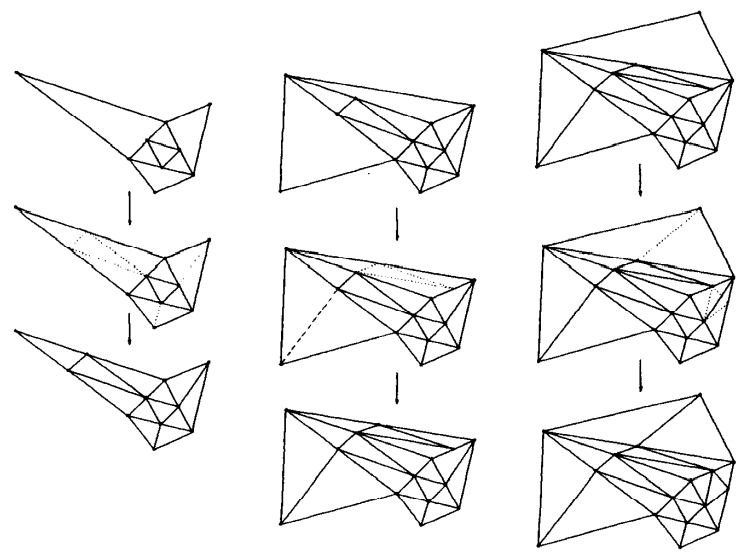
\includegraphics[width=0.9\linewidth]{37}
	\centering
	\label{pfig:ch13_37}
\end{figure}
\textbf{FIGURE 13.50:} Illustration of adaptive mesh refinement scheme of Exercise 27. (a) (left) Step 1, (b) 
(middle) Step 2, and (c) (right) contingency plan for Step 3. 
\\
\\
\\
(iii) Flag those elements whose oscillations are "large" (with respect so some specified indicator, 
say more than double of the average)$^{17}$\footnotetext[17]{We are using a rather basic error indicator. More sophisticated error indicators can be developed 
using advanced techniques of Sobolev spaces; see, for example, [CiLi-89], [Cia-02], or the classical 
reference [StFi-73] for details on such methods. }\\ 
(iv) Refine the mesh accordingly so that each element flagged in (iii) gets split into three similar 
(triangular) elements as in Figure 13.49. Adjacent elements need to be refined accordingly so 
no hanging nodes remain. The two requirements are that the original node set is contained in the 
refined node set and no angle of any element gets too small (eccentricity requirement). 
For defmiteness, let us say that in (iii) the flagging criterion for elements is that the maximum oscillation is more than double the average of all of the oscillations. In (iv) let us say that the eccentricity requirement stipulates that the minimum angle of any refinement cannot be less than $1 / 3$ of the minimum angle, $\theta_{\min }$, of the original triangulation.\\
Balancing these two requirements makes the refinement scheme a delicate task. This sort of a scheme can be accomplished by iteratively applying a series of refinements that attempt (based on the two constraints) to isolate the "hanging nodes." We give an outline for such a scheme:
\\
OUTLINE FOR ADAPTIVE MESH REFINEMENT SCHEME:\\
Step 1: After refining the flagged elements as in (iv), the new nodes introduced need to mesh into the next triangulation. Until they do become vertices of all adjancent elements, they will be referred to as "hanging nodes." Examine all neighboring elements of the flagged elements that were just refined; see Figure 13.50(a). If possible, we would like to contain the spread of green ("hanging nodes") but the problem is that we do not want any of the triangles to have very small angles. For each of the three neighbor triangles, if half the angle of the node opposite the hanging node is not too small $\left(<\theta_{\min } / 3\right)$, then simply split it into two triangles by joining the hanging node of the first triangle to the opposite node of the neighbor triangle (Figure $13.50(\mathrm{a})$ has two such triangles ${ }^{18}$\footnotetext[18]{Note that at the first iteration, this could not occur with the stated eccentricity requirement since bisecting any of the original angles would result in angies at least as large as $\theta_{\min } / 3$; so this pathology in the figure could only occur in later iterations. In particular, for the first refinement, all hanging nodes could be isolated in Step 1 .}). Otherwise, we are forced to refine the neighbor triangle as in (iv), but this introduces two new hanging (green) nodes. (Figure $13.50$ (a) has one of these).\\
Step 2: If Step 1 introduced any new hanging (green) nodes (as it did in Figure $13.50(a)$ ), look at the neighboring triangles and try to contain the hanging nodes as in Step 1. We may again introduce hanging nodes. (Figure 13.50(b) illustrates this). We continue to iterate this step until there are no longer any hanging nodes. There is one contingency we need to mention (if a neighboring triangle runs into another that was already refined), this is illustrated in Figure $13.50(\mathrm{c})$; below we explain what to do in such situations.
Contingency plan for Step 3: Figure $13.50$ (c) illustrates what to do if a neighbor triangle runs into one that was already refined. We do not refine any triangle twice (this will give some control on the convergence of the algorithm and prevent the possibility of an infinite loop). Instead, we revert to the original refinement (three subtriangles instead of two) to take care of the internal green node; see Figure 13.50(c).\\
(a) Write a MATLAB program that will perform the above adaptive scheme on the BVP and initial triangulation of Example 13.5. What happens when you run this program? Repeat, but now change the flagging criterion in (iii) to be that the oscillation of the FEM solution over an element exceeds $1 / 10$. Repeat with $1 / 10$ replaced by $1 / 100$. Plot each refined mesh as well as the final FEM solution.\\
(b) Repeat the instructions of part (a) on the BVP of Exercise 2; compare the final FEM solution with the exact solution given there.\\
(c) Repeat the instructions of part (a) on the BVP of Exercise 3 (using the initial triangulation given there).\\
(d) Do you have any ideas for an altemative mesh refinement scheme (satisfying the two constraints mentioned above)?
	\item (\textit{Obtuse Angles in the Domain Are Sometimes Problematic for the FEM}) Engineers have known 
for some time, and mathematicians subsequently confirmed theoretically, that obtuse comers in 
the domain of a BVP can often slow down the convergence of the FEM near the boundary 
points with obtuse angles (see Section 8.1 of [StFi-73] or Section 5.6 of [AxBa-84]) . Simple 
examples of domains with such obtuse angles are shown in Figure 13.51(b), (c). In general, the 
larger the obtuse angle, the greater the possible problems with the FEM. The extreme case is 
with an interior angle of $2\Pi$ physically corresponding to a crack, fissure, or material interface 
in the domain; see Figure 13.51(c). This exercise will investigate such phenomena and explore 
stategies to mitigate problems that might arise. We will examine a certain Dirichlet problem for the Laplace equation on such a domain where the exact solution is known. For any angle $\omega$, where $0<\omega \leq 2 \pi$, we let $\Omega_{\omega}$ denote the subdomain of all points in the unit square $-1 \leq x, y \leq 1$ whose polar coordinates $(r, \theta)$ satisify $0<\theta<\omega$. Thus the domains of Figure $13.51$ are all examples of such domains. In particular, the domain in Figure 13.51(b) is $\Omega_{3 \pi / 2}$ and that of Figure $13.51$ (c) is $\Omega_{2 \pi}$.
(a) Show that on any such domain $\Omega_{\omega}$ the function (given in polar coordinates) $u(r, \theta)=r^{\pi / \omega} \sin (\pi \theta / \omega)$ is harmonic (i.e., satisfies the Laplace equation $\Delta u=0$ ) and vanishes on the angular edges (i.e., the rays of the angle emanating from the point $O$; see Figure 13.51.).\\
(b) For each of the domains in Figure $13.51$ (for the one in Figure 13.51(a) use $\omega=2 \pi / 3$ ), apply the FEM to solve BVP consisting of the Laplace equation with the boundary conditions $u$ $=0$ on the angular edges of the boundary and $u(r, \theta)=r^{\pi / \omega} \sin (\pi \theta / \omega)$ on the remaining portion of the boundary. Of course, you will need to convert the latter boundary conditions into cartesian $(x, y)$ coordinates. Start off with the corresponding triangulations shown in Figure 13.52. Then apply the algorithm of Exercise 25 to successively refine the triangulations and resolve with the FEM. For each triangulation, plot the exact error using the exact solution in part (a). Go through three refinements for each domain.\\
(c) Repeat part (b) for each of the three BVPs given there, but this time using the adaptive scheme of Exercise 27 in place of the refinement scheme of Exercise 25.\\
(d) Using the special form of the triangulations given, can you think of a more convenient refinement scheme for this problem? Make up a reasonable one and test it out for several iterations comparing with the exact solution at each step.
Suggestion: An elegant and illuminating way to do part (a) is to derive the Laplace operator in polar coordinates to be: $u_{x x}+u_{y y}=u_{r r}+(1 / r) u_{r}+\left(1 / r^{2}\right) u_{\theta \theta}$.
\begin{figure}[H]
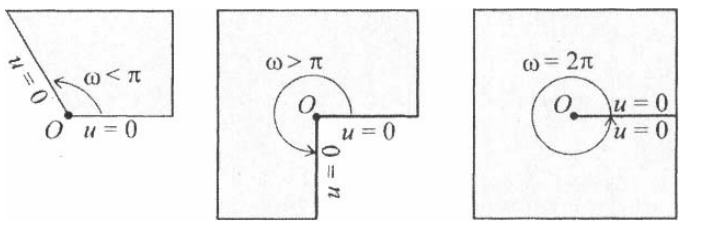
\includegraphics[width=0.9\linewidth]{38}
	\centering
	\label{pfig:ch13_38}
\end{figure}
\textbf{FIGURE 13.51:} Simple examples of domains with different sorts of angles at a boundary point O. (a) 
(left) In general acute angles do not pose any problems for the FEM. (b) (middle) Obtuse angles can 
sometimes lead to slower convergence of the FEM. (c) (right) The larger the obtuse angle, the greater 
the potential difficulty. The extreme case is the slit domain. The indicated homogeneous Dirichlet 
boundary conditions on the angular edges is relevant for Exercise 28. 
\\
\\
\begin{figure}[H]
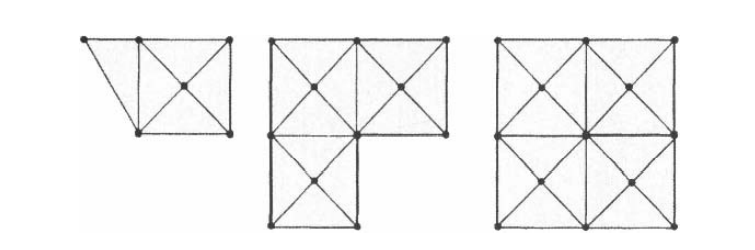
\includegraphics[width=0.9\linewidth]{39}
	\centering
	\label{pfig:ch13_39}
\end{figure}
\textbf{FIGURE 13.52:} Initial triangulation for the domains of Figure 13.51 for Exercise 28.
	\item Suppose that the FEM of this section is used to compute the solution of a BVP of form (10) whose exact solution is known to be a linear function $u(x, y)=a x+b y+c$. Assume the integrals are all computed exactly and that the domain and triangulation are such that the boundary of the domain consists entirely of edges of the triangulation. Will the FEM solution always coincide with the exact solution? Either explain whether this is true or, if you are unable to do so, perform a series of numerical experiments to test this hypothesis.\\
\textbf{Note:} Since the basis functions are piecewise linear, this seems to be the most general type of solutions that the FEM might be able to produce exactly. An example of such a BVP and triangulation is given in Exercise $1 .$
\end{enumerate}
\newpage
\section*{Appendix A: Introduction to MATLAB's 
Symbolic Toolbox }
\textbf{A.l: WHAT ARE SYMBOLIC COMPUTATIONS?}
\\
\\


This appendix is meant as a quick reference for occasions in which exact 
mathematical calculations or manipulations are needed and are too arduous to 
expediently do by hand. Examples include the following: 
\begin{enumerate}
	\item Computing the (formula) for the derivative or antiderivative of a function
	\item Simplifying or combining algebraic expressions
	\item Computing a definite integral exactly and expressing the answer in terms of known functions and constants such as $\pi, e, \sqrt{7}$ (if possible)
	\item Finding analytical solutions of differential equations (if possible)
	\item Solving algebraic or matrix equations exactly (if possible)
\end{enumerate}
Such exact arithmetic computations are known collectively as \textbf{symbolic computations}. MATLAB is unable to perform symbolic computations but the Symbolic Math Toolbox is available (or included with the Student Version), which computing system. Thus, MATLAB has essentially subcontracted symbolic computations to MAPLE, and acts as a "middleman" so that it is not necessary to use two separate softwares while working on problems. Invoking such symbolic capabilities needs specific actions on the user's part, such as declaring certain variables to be symbolic variables. This is a safety device since symbolic calculations are usually much more expensive than the default floating point calculations and are usually not called for (see Chapter 5 ). It is important to point out that symbolic expressions are different data types than the other sorts of data types that MATLAB uses. Consequently, care needs to be taken when passing data from one type of data to the other. Moreover, most mathematical problems have answers that cannot be expressed in terms of well-known functions (e.g., $\ln (x), \sqrt{x}, \arcsin (x))$ and/or constants (e.g., $e, \pi, \sqrt{2})$, and therefore cannot be solved symbolically.
\\
\\
There are also circumstances where the precision of MATLAB's floating point 
arithmetic is not good enough for a given computation and we might wish to work 
in more than the 15 (or so) significant digits that MATLAB uses as a default. As a 
middle ground between this and exact arithmetic, the Symbolic Toolbox also 
offers what is called variable precision arithmetic, where the user can specifyhow many significant digits to work with. We point out that there are a few 
special occasions where symbolic calculations have been used in the text.\\ 
The remainder of this appendix will present a brief survey of some of the 
functionality and features of the Symbolic Toolbox that will be useful for our 
needs. All of the MATLAB code and output given in a particular section results 
from a new MATLAB session having been started at the beginning ofthat section.
\\
\\
\textbf{A.2: ANALYTICAL MANIPULATIONS AND CALCULATIONS }
\\
\\
To begin a symbolic calculation, we need to declare the relevant variables as 
symbolic. To declare x, y as symbolic variables we enter: \\
\\
\texttt{>> syms x y}
\\
\\
Let's now do a few algebraic manipulations. The basic algebra manipulation 
commands that MAPLE has are as follows: \texttt{expand},\texttt{factor},\texttt{simplify}; they 
work on algebraic expressions just as anyone who knows algebra would expect. 
The next examples will showcase their functionality. We point out that any new 
variable introduced whose formula depends on a symbolic variable will also be 
symbolic. 
\\
\\
\texttt{>> $p2=(x+2*y)^{\wedge}2 ; , p4= (x+2*y)^{\wedge}4;$ }\\
\texttt{>> expand(p2) \%Multiplies out the binomial product. }\\
\texttt{->ans = $x^{\wedge}2+4*x*y+4*y^{\wedge}2$}\\
\texttt{>> expand(p4)}\\
\texttt{-> $ans=x^{\wedge}4+8*x^{\wedge}3*y+24*x^{\wedge}2*y^{\wedge}2+32*x*y^{\wedge}3+16*y^{\wedge}4$}\\
\texttt{>> pretty(ans) \%Puts the answer in a prettier form.}\\
\texttt{>> 4 ~3~ 2 2 ~3~ 4 }\\
\texttt{x + 8 x y + 24 x y + 32 x y +16y}
\\
\\
In general, for any sort of analytical expression exp, the command 
expand (exp) will use known analytical identities to try and rewrite exp in a 
form in which sums and products are expanded whenever possible. 
\\
\\
\texttt{>> prett y (expand (tan ($x+2*y$) ))->}
$$
\frac{\tan (x)+2 \frac{\tan (y)}{1-\tan (y)}}{} \frac{\tan (x) \tan (y)}{1-2-\tan (y)^{\wedge}2}
$$
To clean up (simplify) any sort of analytical expression (involving powers, 
radicals, trig functions, exponential functions, logs, etc.), the \texttt{simplify} function 
is extremely useful. 
\texttt{>> simplify(log($2*sin(x)^{\wedge}2+cos(2*x)))$~~->ans=0 }\\
\texttt{>> $h=x 6-x^{\wedge}5-12*x^4-2*x^{\wedge}3+41*x^{\wedge}2+51*x+18;$ }\\
\texttt{>> pretty(factor(h)) }\\
\texttt{->  ~~2 ~~~ 3 }\\
\texttt{(x+2(x-3)(x+1)}\\
\\
This function will also factor positive integers into primes. This brings up an important point. MATLAB also has a function factor that (only) does this latter task. Due to the limitations of floating point arithmetic, MATLAB's version is more restrictive than MAPLE's; it is programmed to give an error if the input exceeds $2^{32} \approx 4.2950 \mathrm{e}+009$.
\\
\\
\texttt{>> factor(3$^{\wedge}$101-1) }\\
??? Error using ==> factor \\
The maximum value of n allowed is 2$^{\wedge}$32\\
\texttt{>> factor(sym(3$^{\wedge}$101-1)) \%declaring the integer input as symbolic 
}\\
\texttt{\%brings forth the MAPLE version this command. 
}\\
\texttt{>>ans = (2)$^{\wedge}110^*(43)^*(47)^*(89)^*(6622026029) $}
\\
\\
Whereas the Student Version of MATLAB includes access to many of the 
Symbolic Toolbox commands that one might need to supplement MATLAB 
functionality, the complete Symbolic Toolbox (for MATLAB's professional 
version) includes unrestricted access to all of MAPLE's commands. AH of the 
Symbolic Toolbox commands that we discuss in this Appendix are available with 
the Student Version. To learn more about additional Symbolic Toolbox 
commands available on the version of MATLAB that you are using, consult the 
Help menu. 


	
	






\end{document}
